\section{Messaufbau Resultate}
In diesem Kapitel werden die Messresultate des Laboraufbaus analysiert und mit den Simulationen und den Normen verglichen. Hierbei wurden die Daten der Messungen als .csv Datei gespeichert um mit Matlab die Signale schön darstellen zu können und das FFT berechnen zu können. 

\subsection{Messungen Spannungen}
Um die Werte des Laboraufbaues mit den Simulationen vergleichen zu können, wurden die Spannungen beim Widerstand und bei der ASM gemessen. Dafür wurden die Spannungssignale als Grafik und als Tabelle mit den Werte des FFTs bei den Harmonischen Oberwellen dargestellt.

\subsubsection{Messungen Widerstand}
Für die Messungen mit dem Widerstand, werden bei der Phasenanschnittsteuerung die Winkel 60\textdegree \hspace{0.02cm} und 90\textdegree \hspace{0.02cm} mit den Simulationen verglichen. Für die Schwingungspaketsteuerung wurde ein Duty cycle von 0.5 und 0.8 verglichen. Desweiteren werden noch der normale und der Langsame Sanft-Anlasser analysiert.


\subsubsection*{Phasenanschnitt 60\textdegree}

\begin{figure}[ht!]
	\centering
	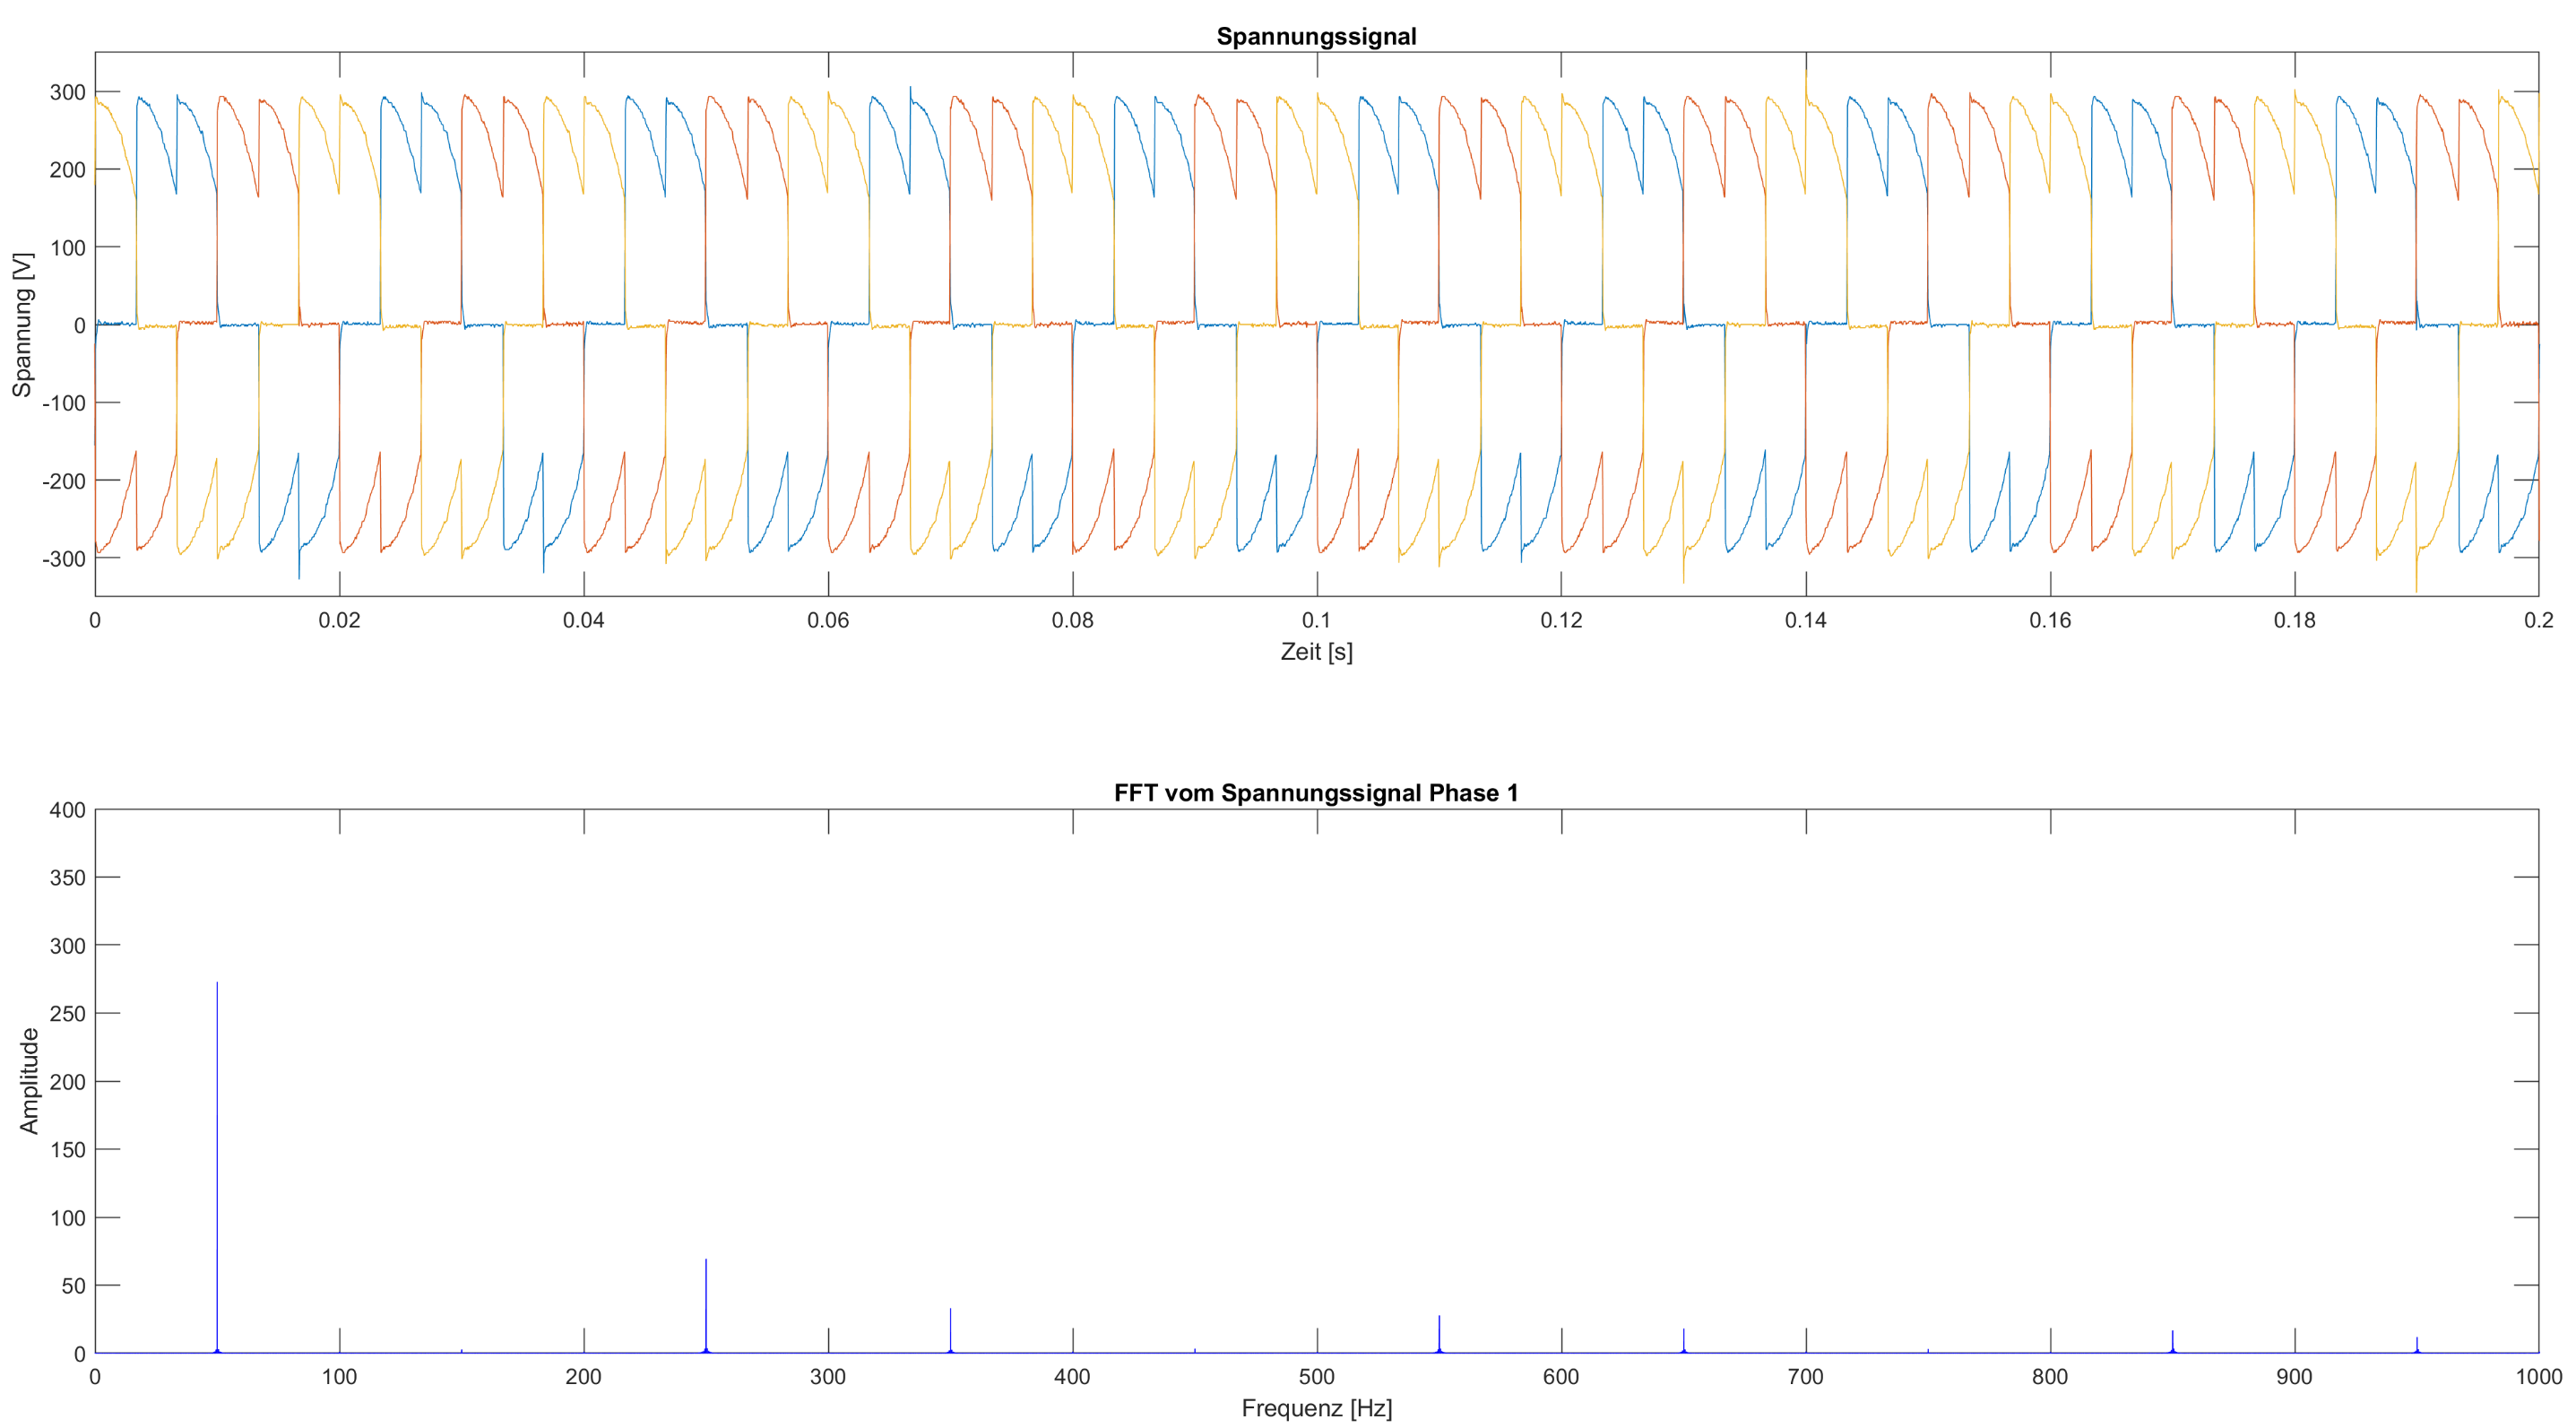
\includegraphics[width=\textwidth]{Messung_Widerstand_Phas_60grad.png}	
	\caption{Messung mit Phasenanschnitt 60\textdegree}\label{fig:Mess_Phas_60}
\end{figure}
\newpage
\subsubsection*{Phasenanschnitt 90\textdegree}
\begin{figure}[ht!]
	\centering
	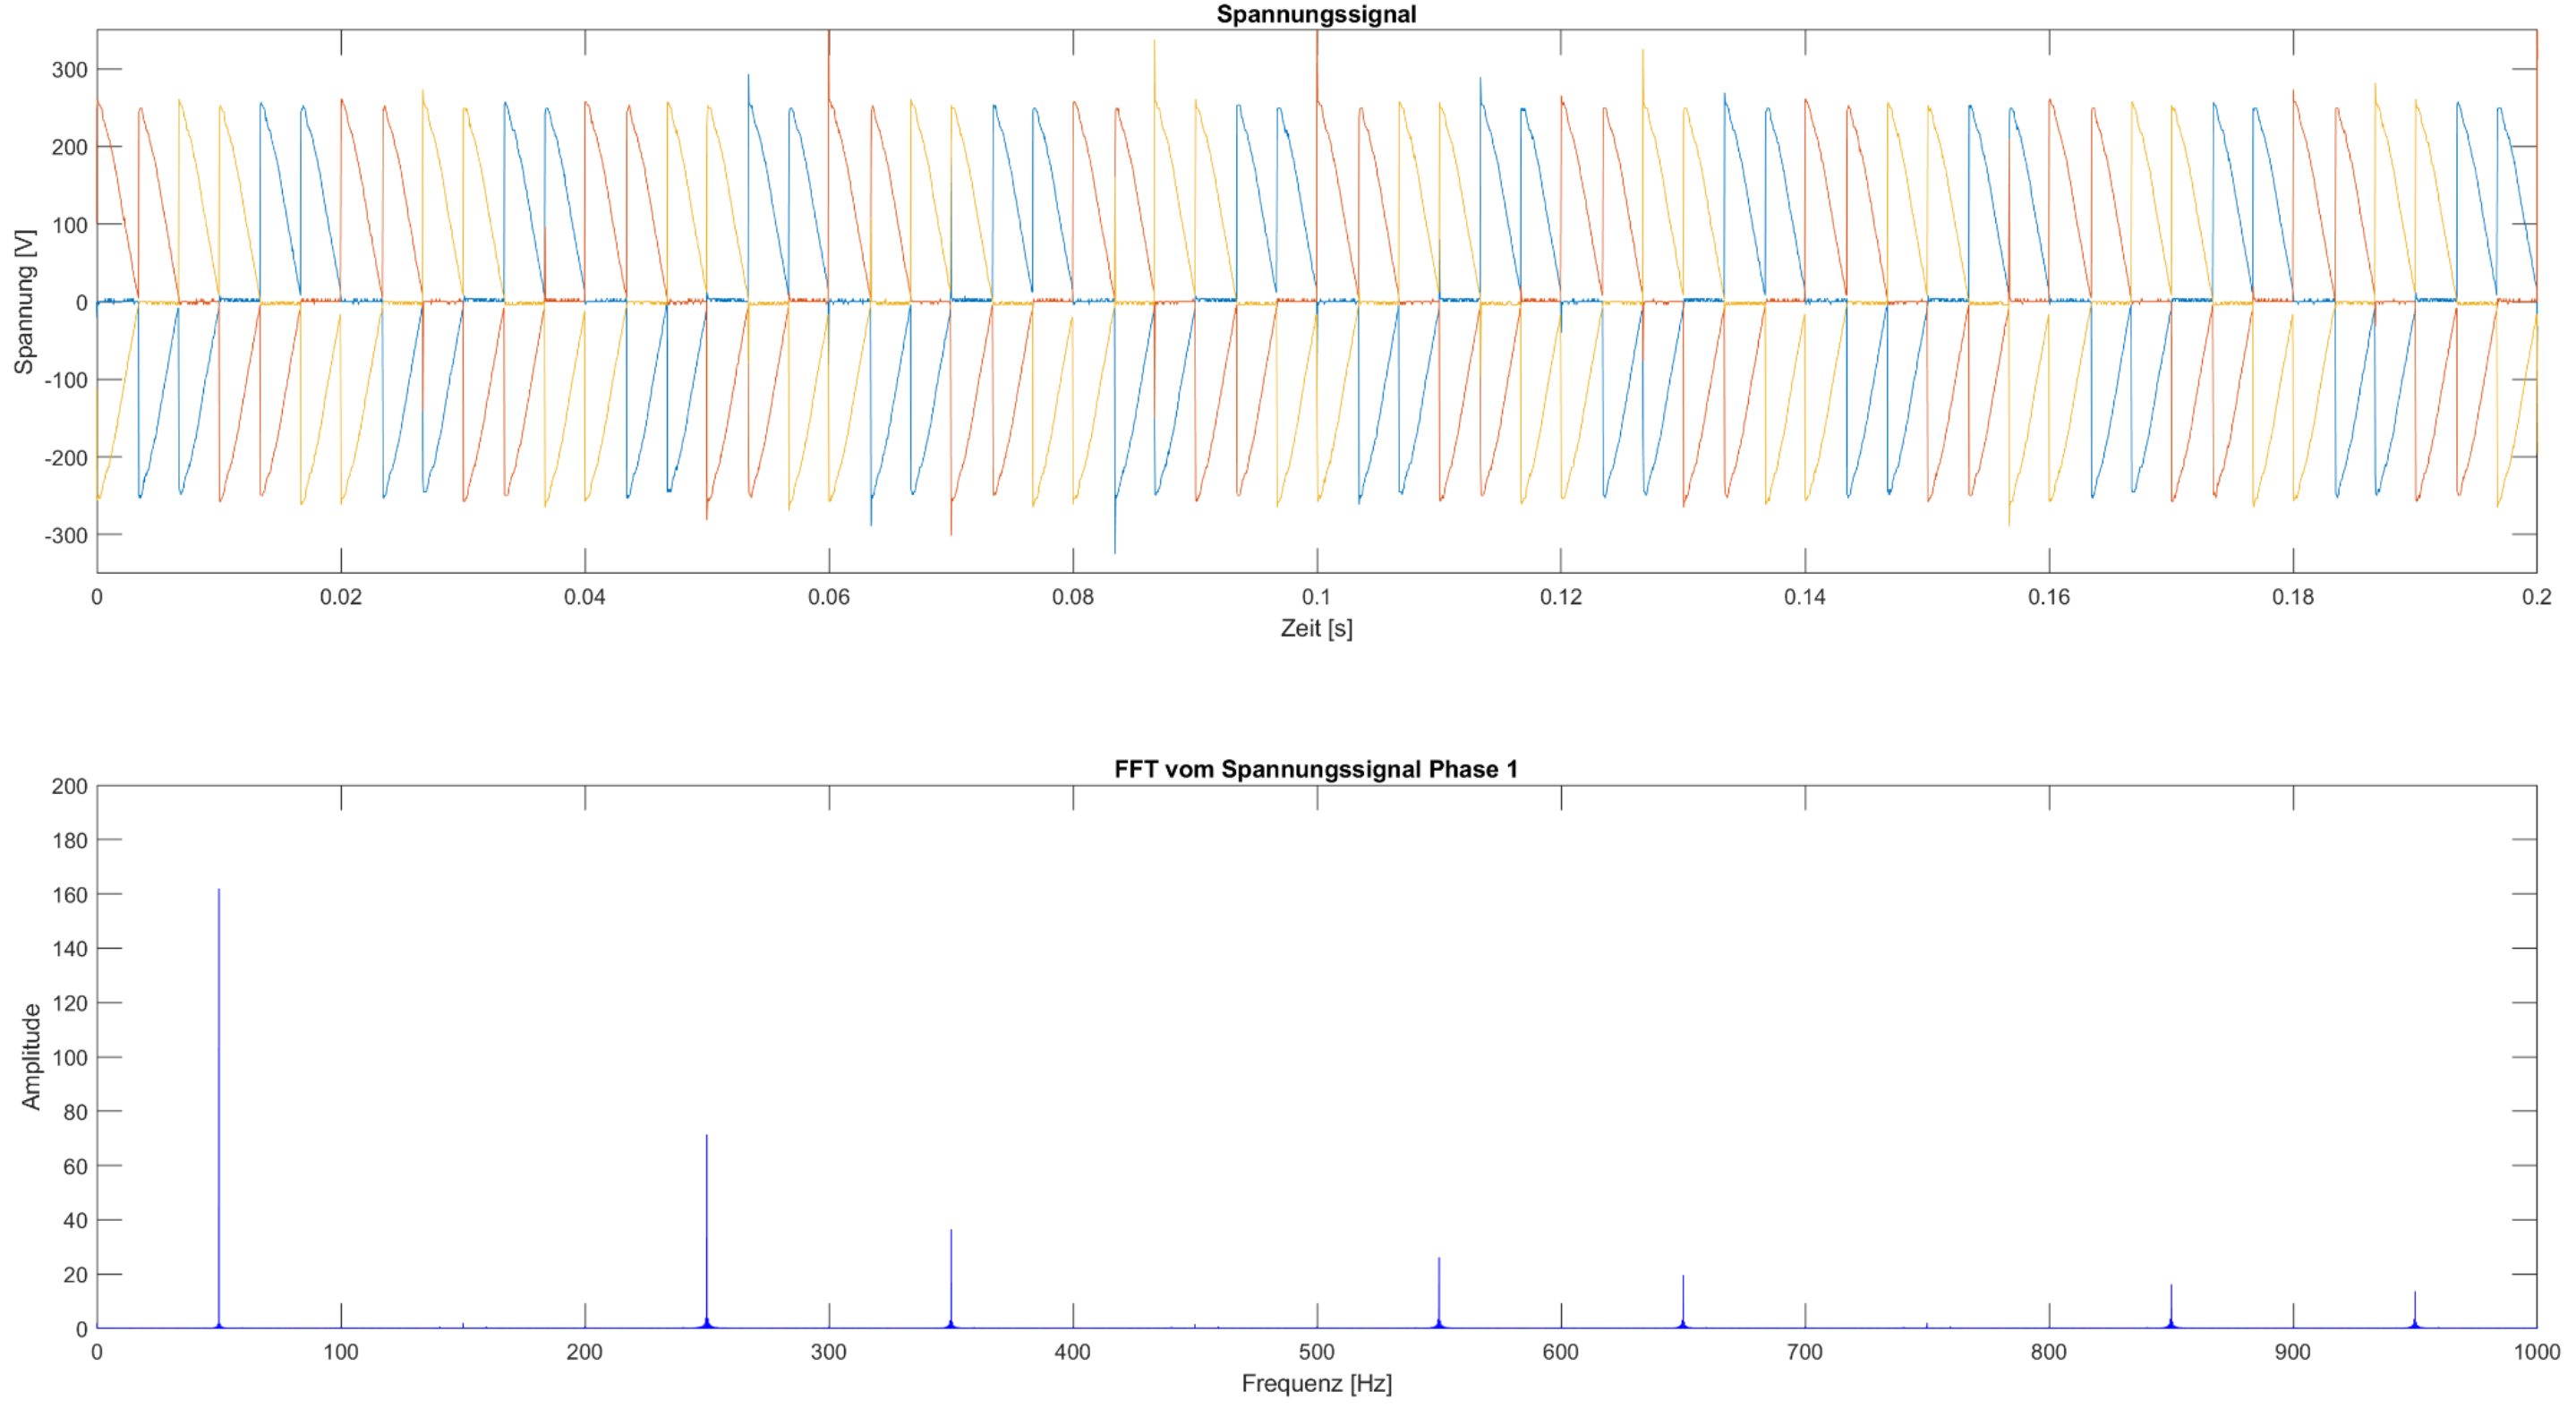
\includegraphics[width=\textwidth]{Messung_Widerstand_Phas_90grad.png}	
	\caption{Messung mit Phasenanschnitt 90\textdegree}\label{fig:Mess_Phas_90}
\end{figure}

\newpage
\subsubsection*{Schwingungspaket 50\%}
\begin{figure}[ht!]
	\centering
	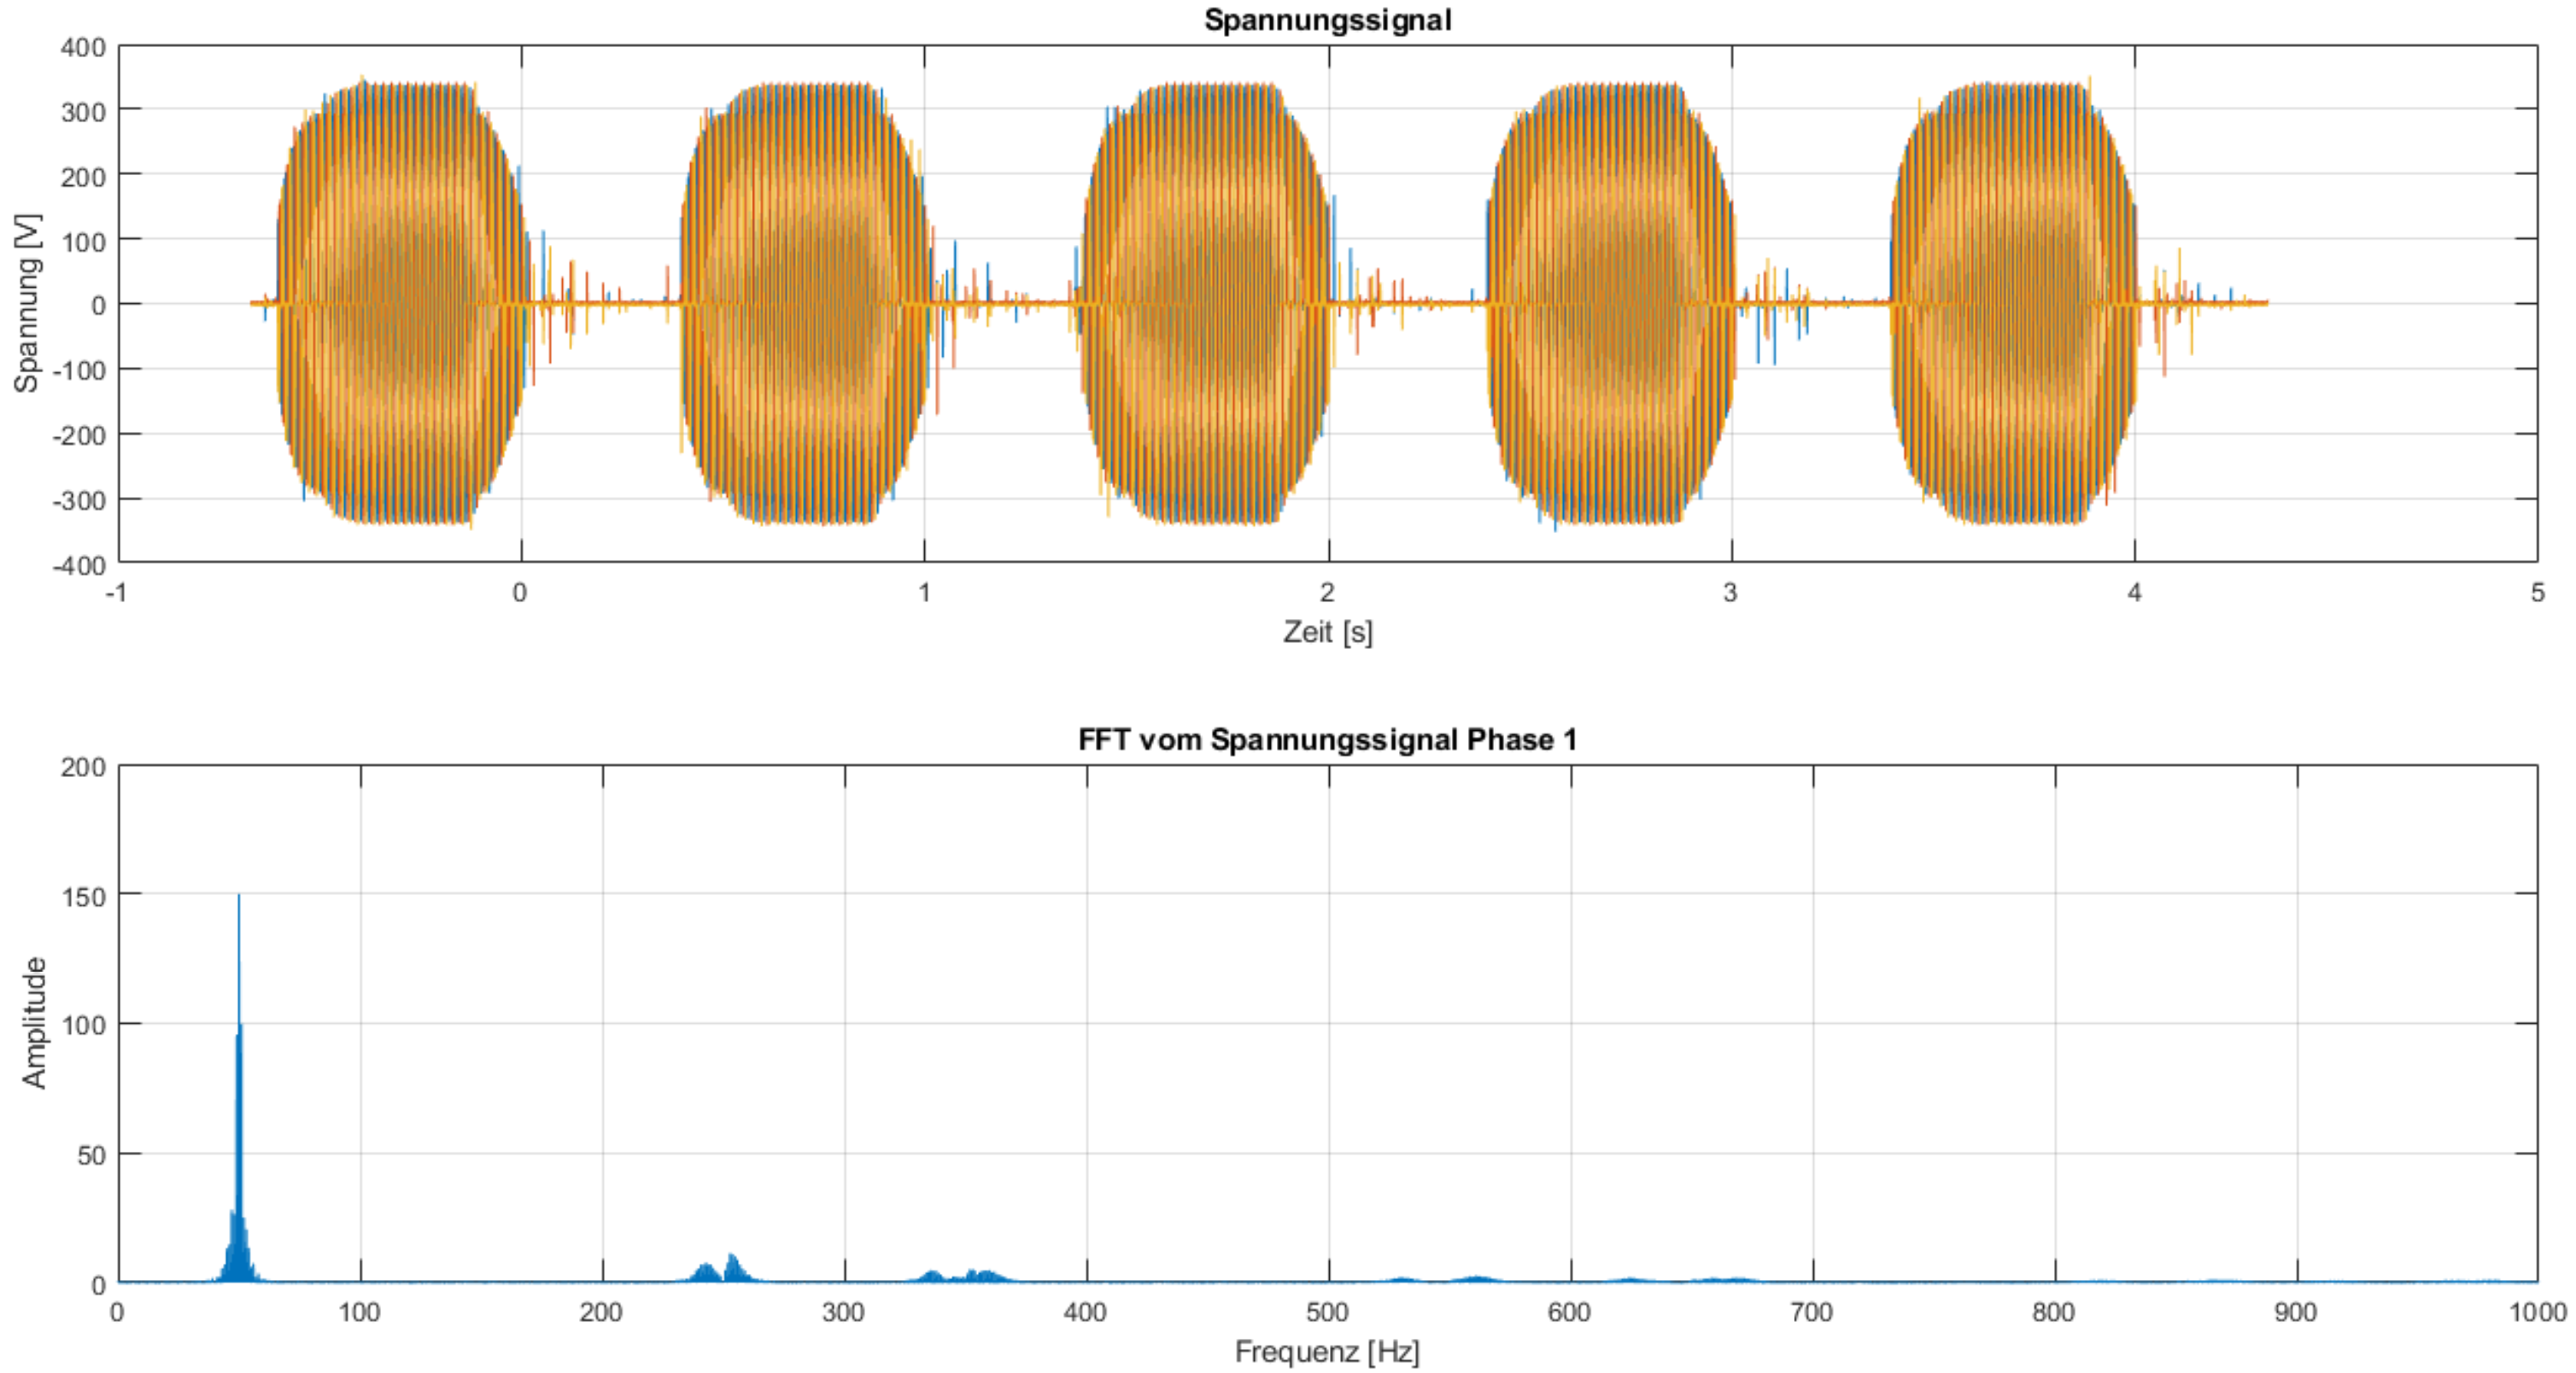
\includegraphics[width=\textwidth]{Messung_Widerstand_Schwing_0_5.png}	
	\caption{Messung mit Schwingungspaket 50\%}\label{fig:Mess_Schwing_50}
\end{figure}

\newpage
\subsubsection*{Schwingungspaket 80\%}
\begin{figure}[ht!]
	\centering
	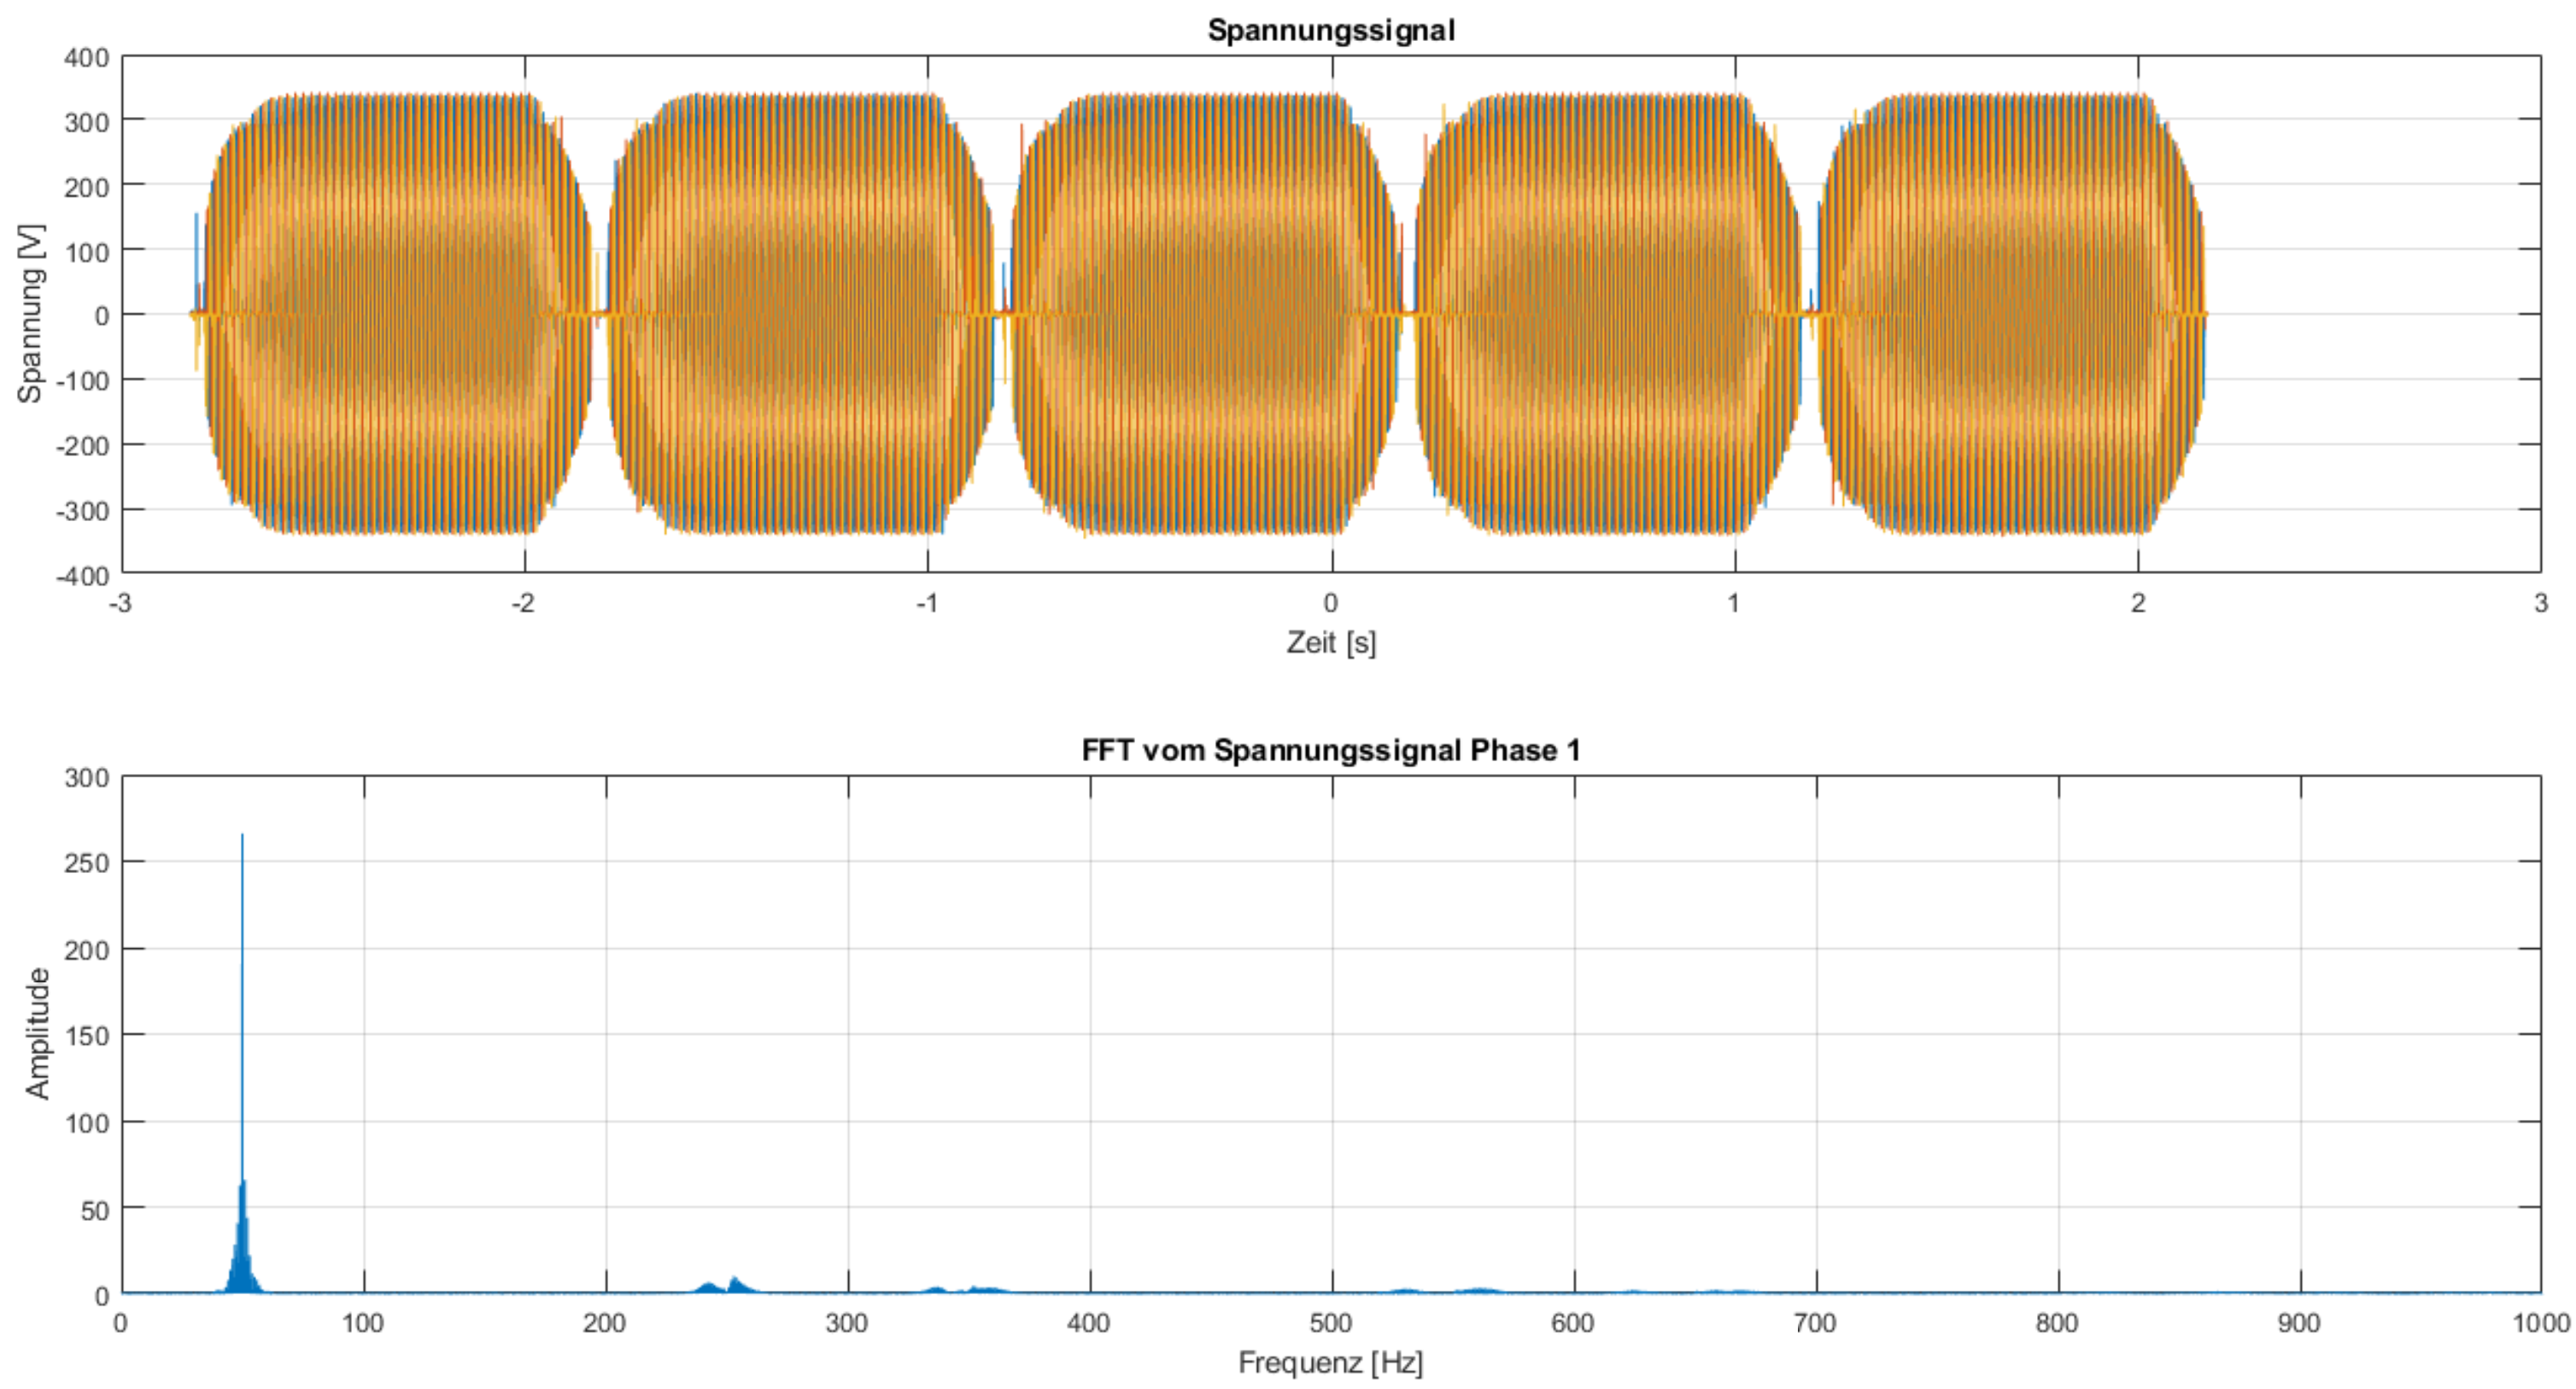
\includegraphics[width=\textwidth]{Messung_Widerstand_Schwing_0_8.png}	
	\caption{Messung mit Schwingungspaket 80\%}\label{fig:Mess_Schwing_80}
\end{figure}

\newpage
\subsubsection*{Sanft-Anlasser}
\begin{figure}[ht!]
	\centering
	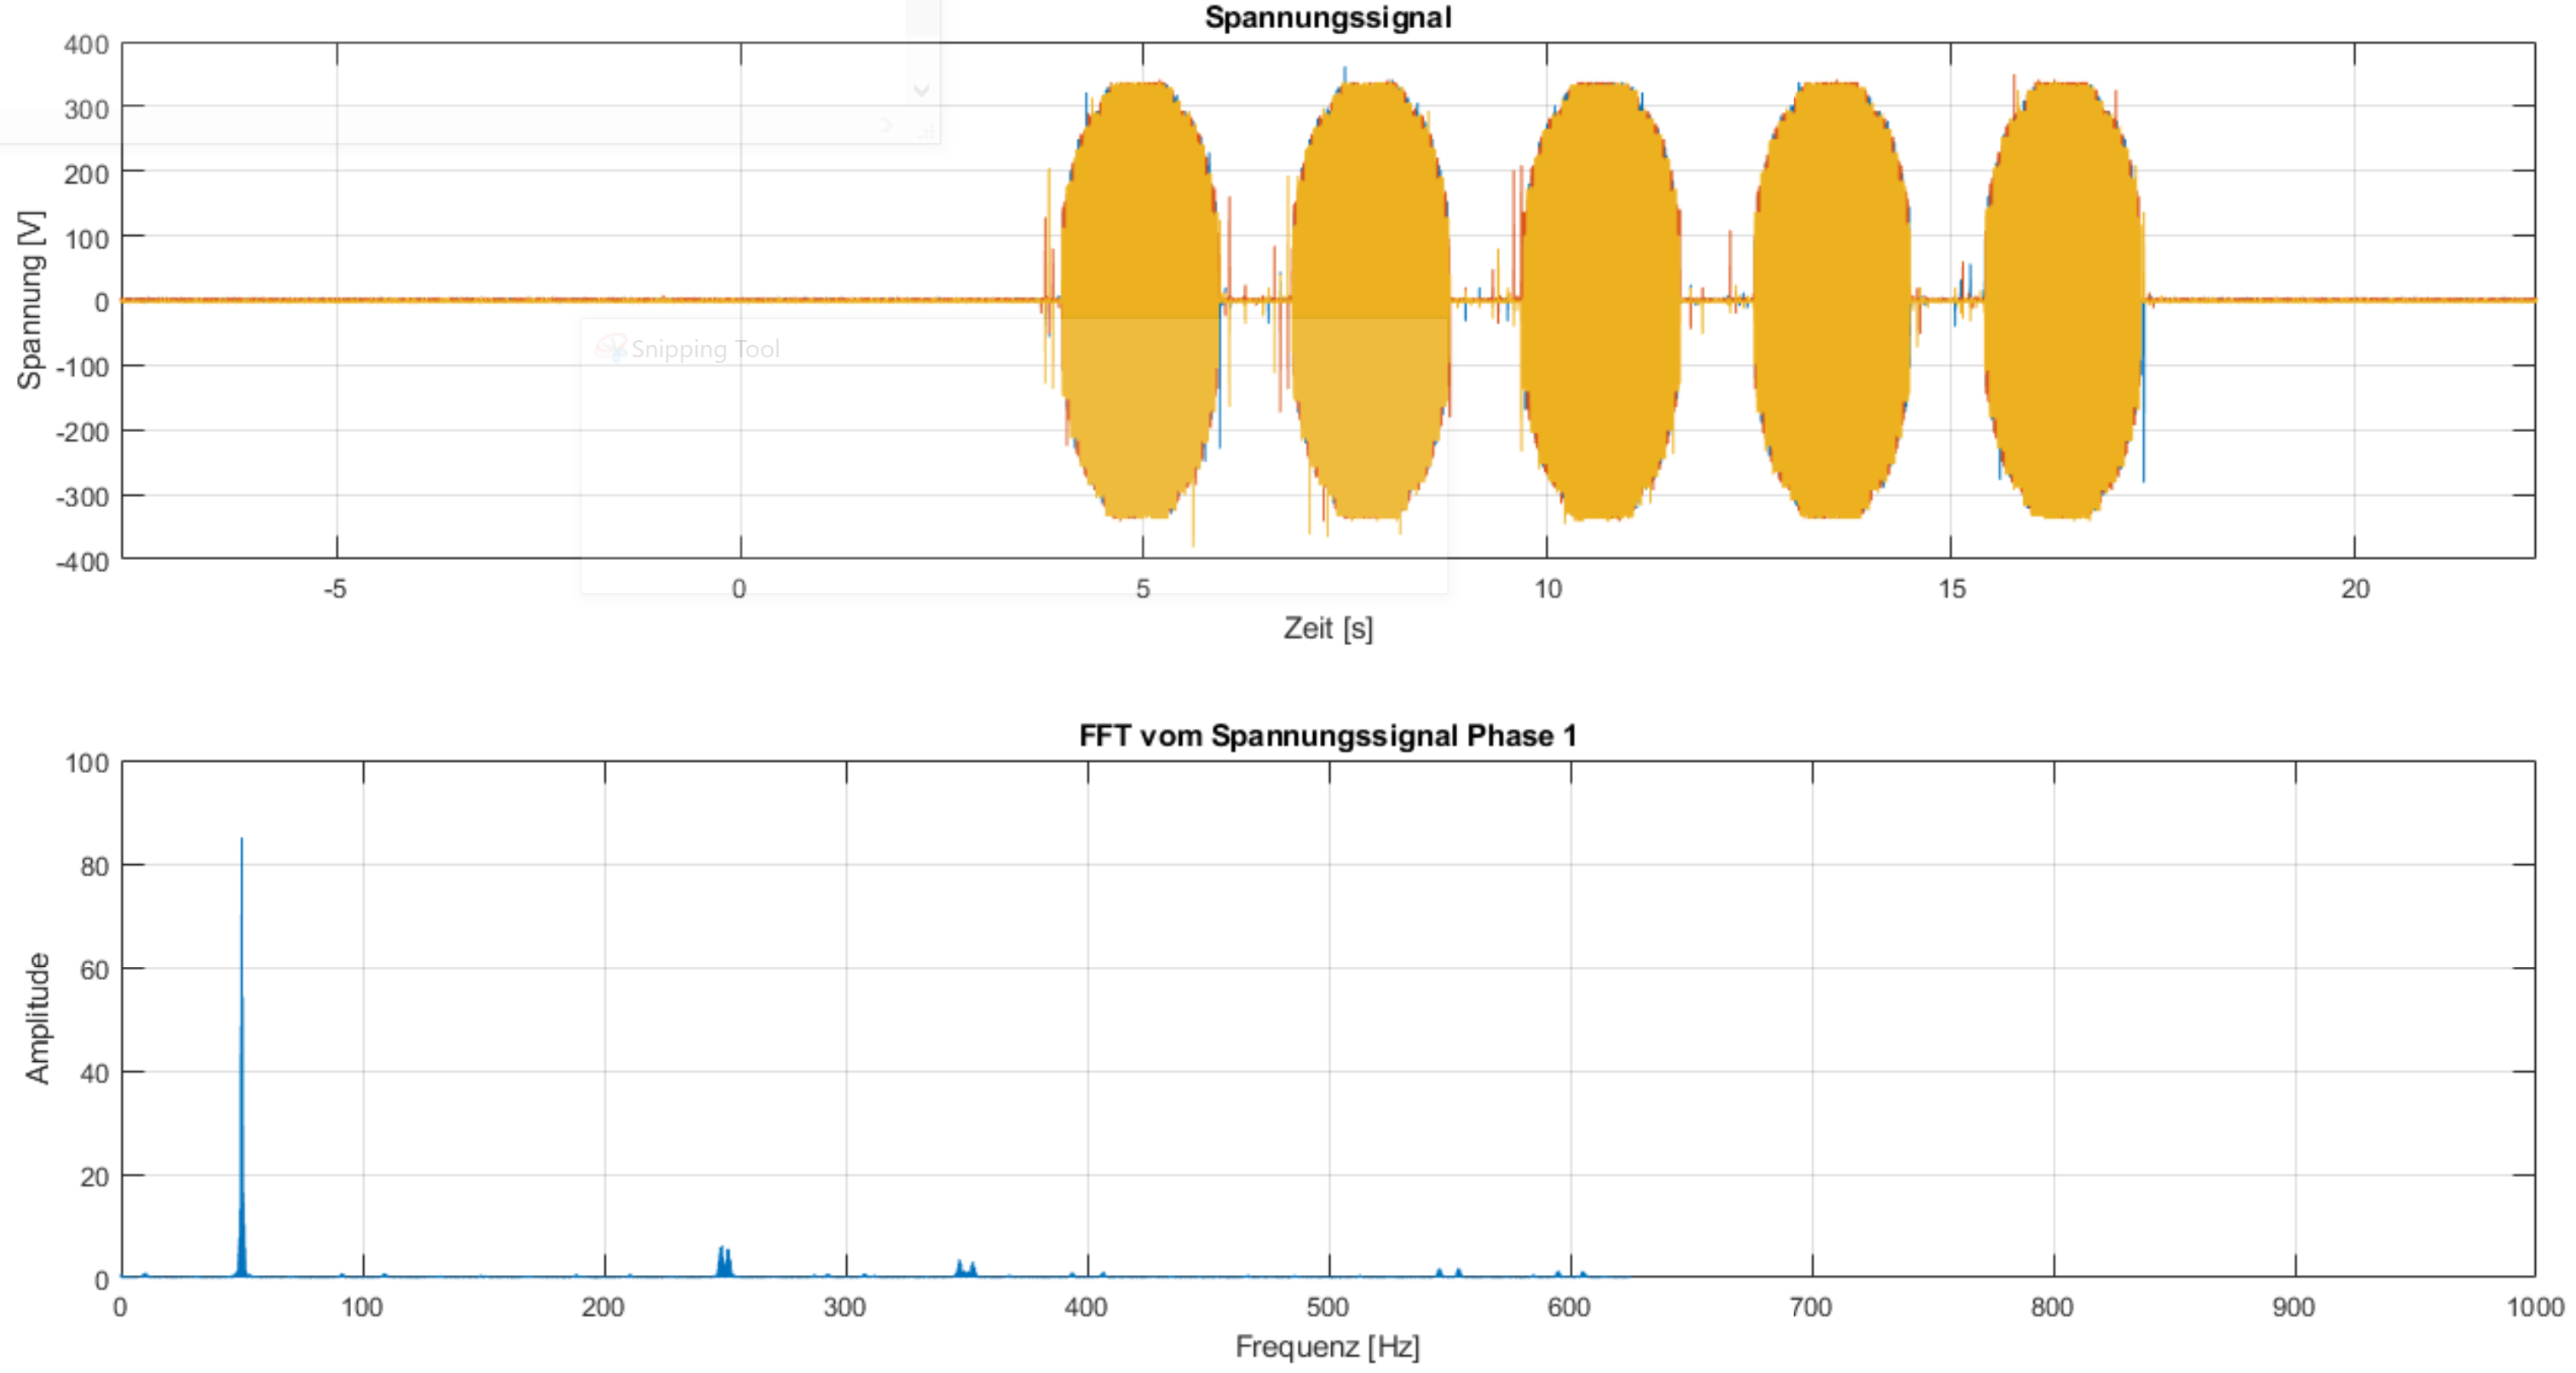
\includegraphics[width=\textwidth]{Messung_Widerstand_Sanft.png}	
	\caption{Messung mit Sanft-Anlasser}\label{fig:Mess_Sanft}
\end{figure}

\newpage
\subsubsection*{Sanft-Anlasser Langsam}
\begin{figure}[ht!]
	\centering
	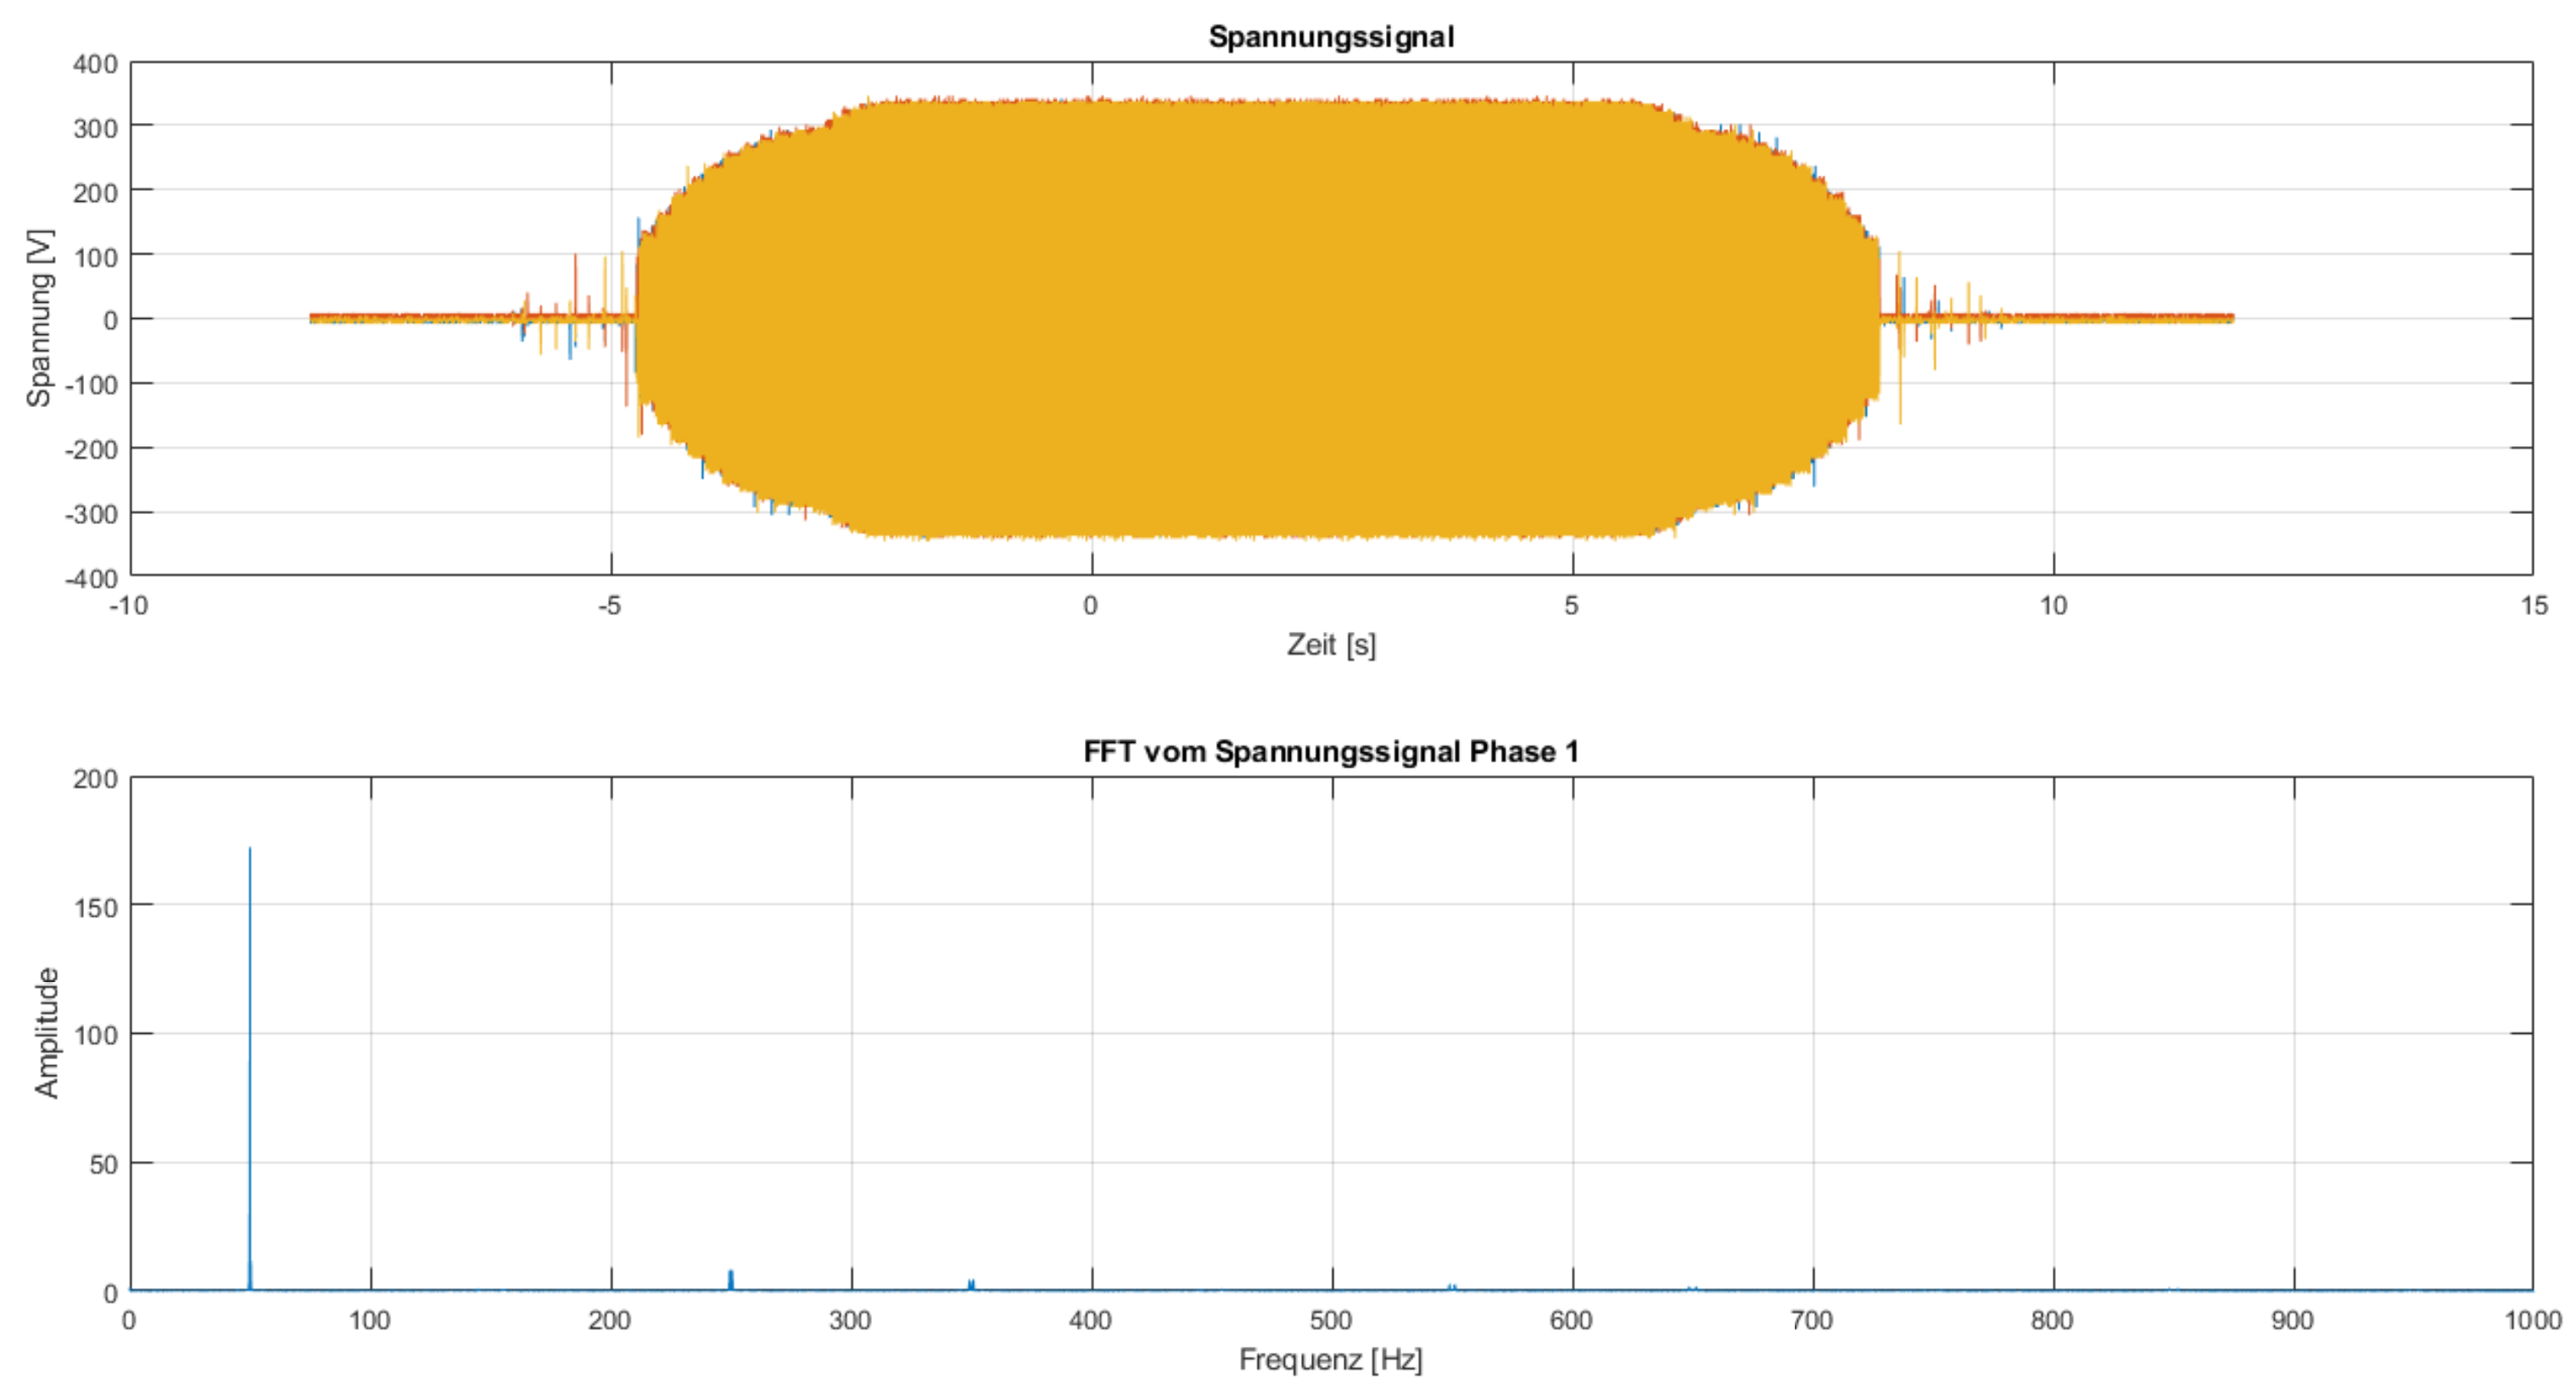
\includegraphics[width=\textwidth]{Messung_Widerstand_Sanft_langsam.png}	
	\caption{Messung mit Sanft-Anlasser langsam}\label{fig:Mess_Sanft_langsam}
\end{figure}

\newpage
\subsubsection{Messungen ASM}
Um zu analysieren, wie sich der Thyristorsteller bei einer ohmsch-induktiver Last verhält, wurden die Messungen mit einer ASM gemacht. Auch hier wurden die verschiedenen Ansteuerungsarten, Phasenanschnitt mit 60\textdegree \hspace{0.02cm} und 90\textdegree \hspace{0.02cm}, Schwingungspaket mit 50\% und 80\%, und dem normalen und langsamen Sanft-Anlasser. Dabei wurde schnell festgestellt, dass die Schwingungspaketsteuerung und der normale Sanft-Anlasser sich nicht für eine ASM eignen. \todo{Begründen wieso nicht}


\subsubsection*{Phasenanschnitt 60\textdegree}
\begin{figure}[ht!]
	\centering
	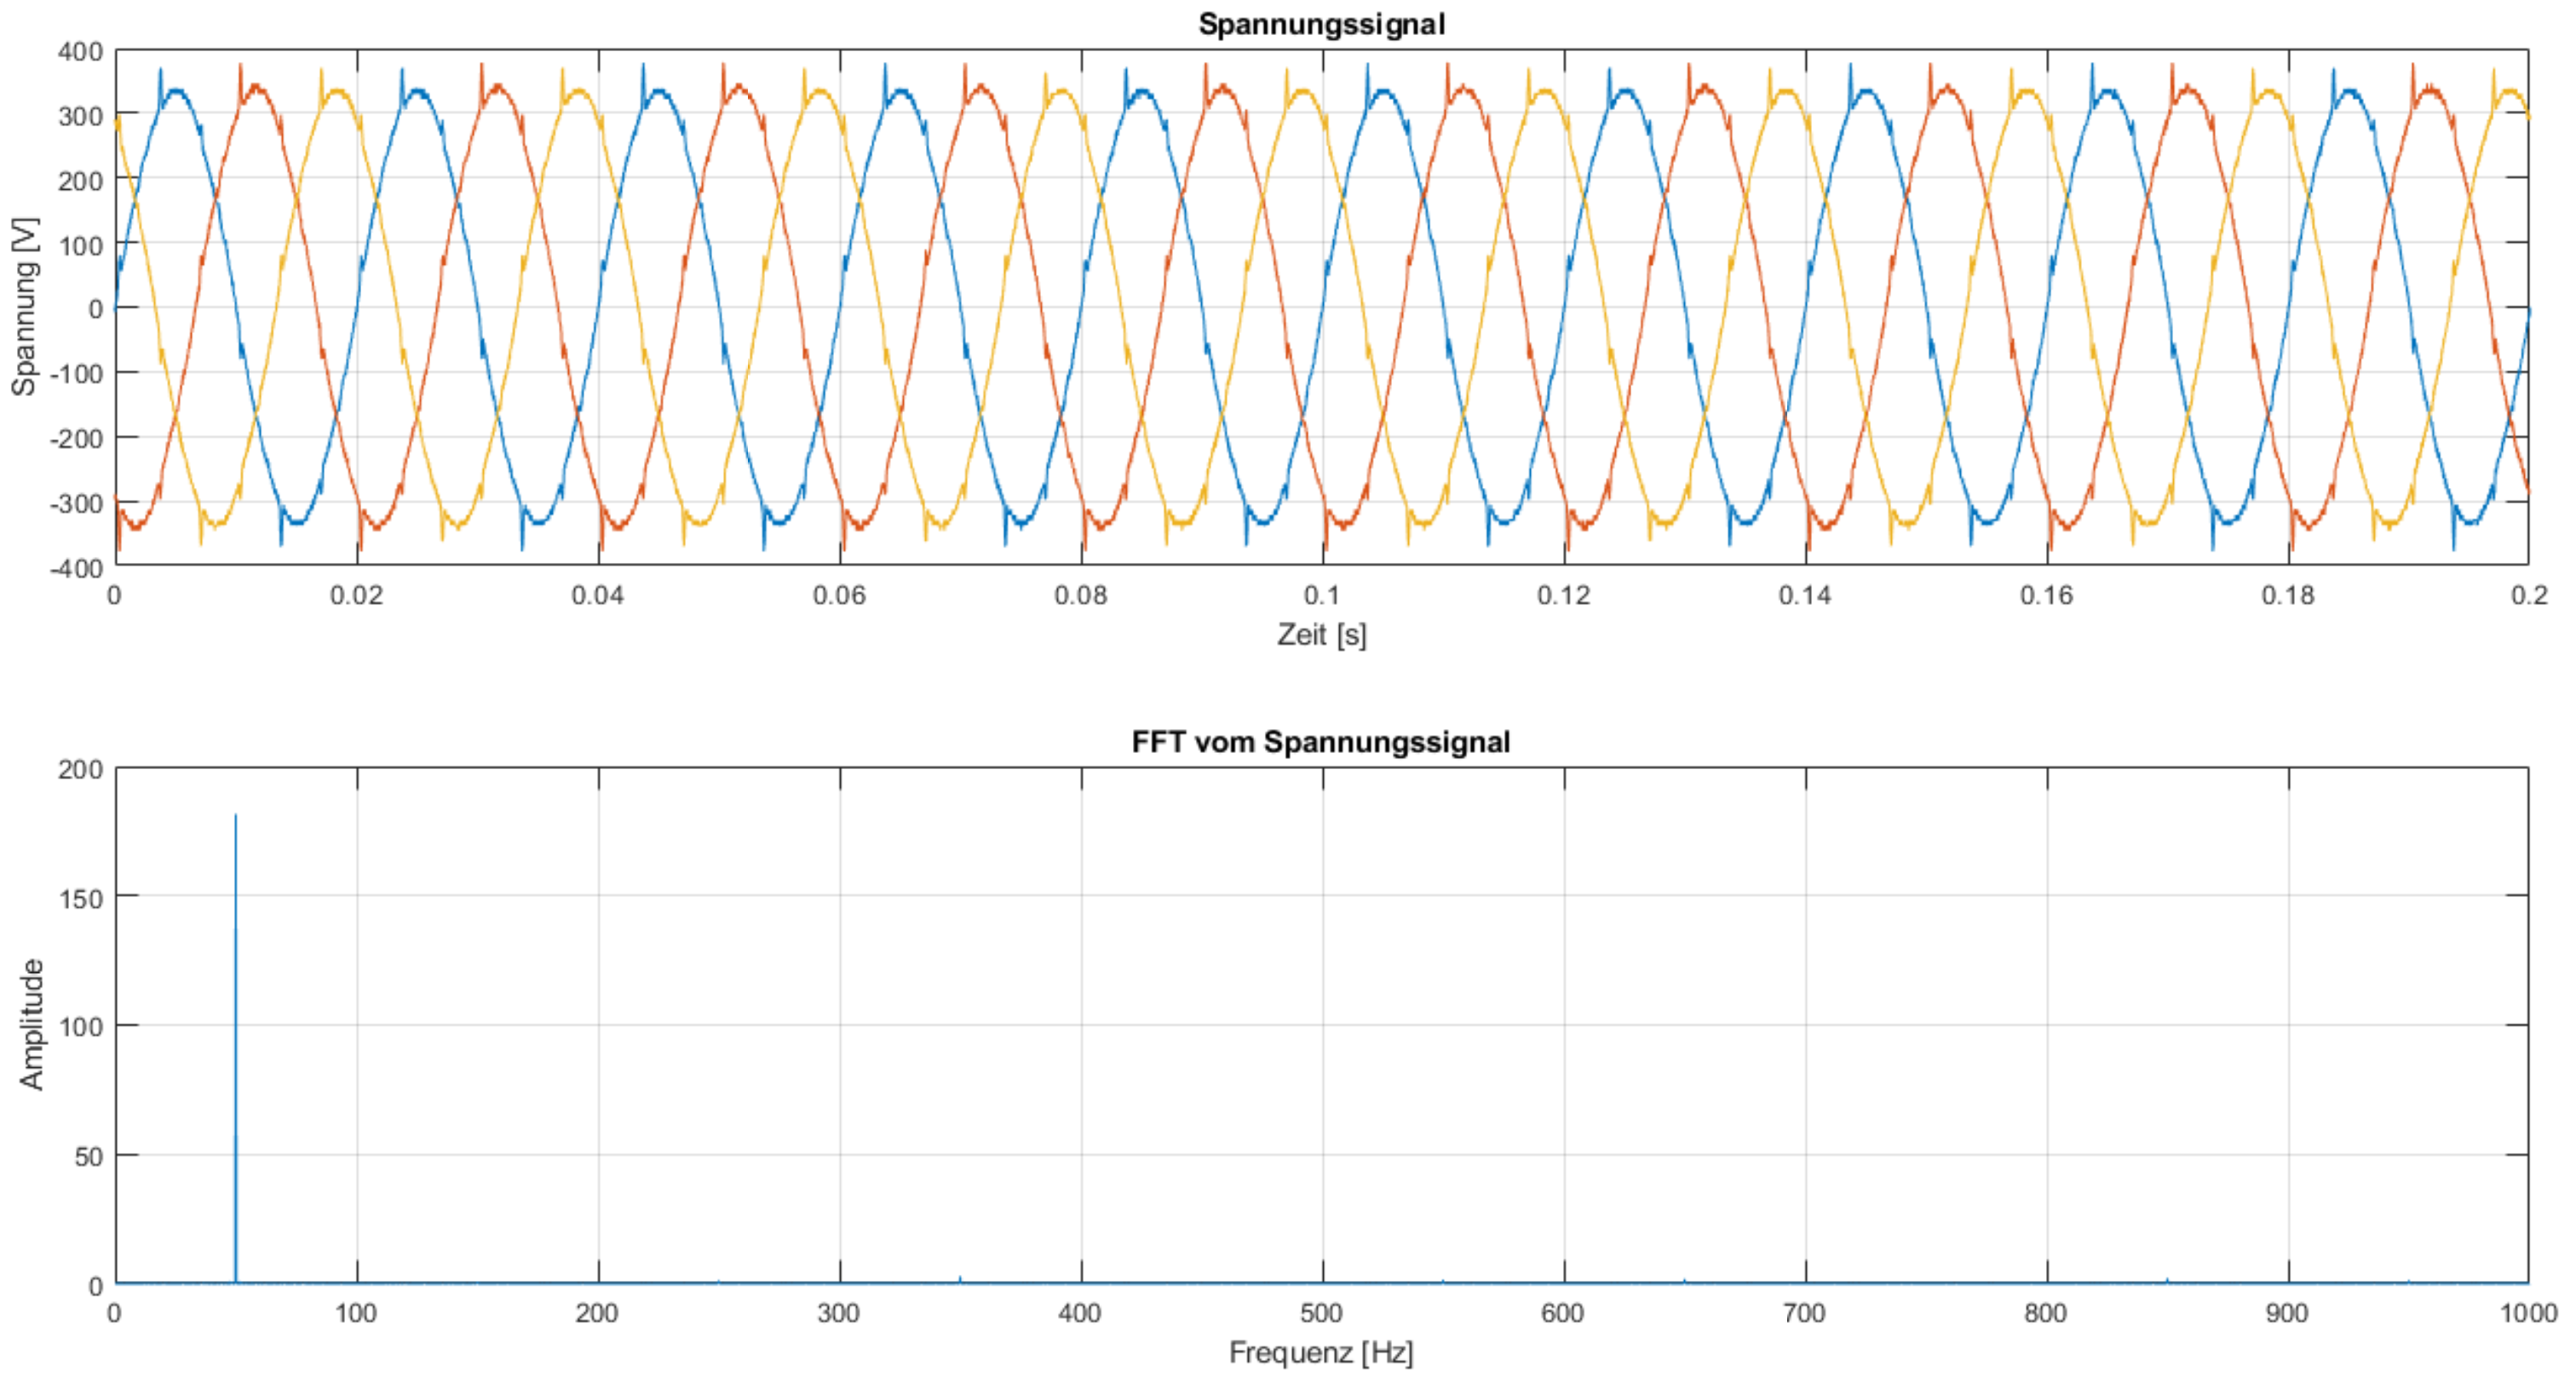
\includegraphics[width=\textwidth]{Messung_ASM_Phas_60grad.png}	
	\caption{Messung mit Phasenanschnitt 60\textdegree}\label{fig:Mess_ASM_Phas60}
\end{figure}

\newpage
\subsubsection*{Phasenanschnitt 90\textdegree}
\begin{figure}[ht!]
	\centering
	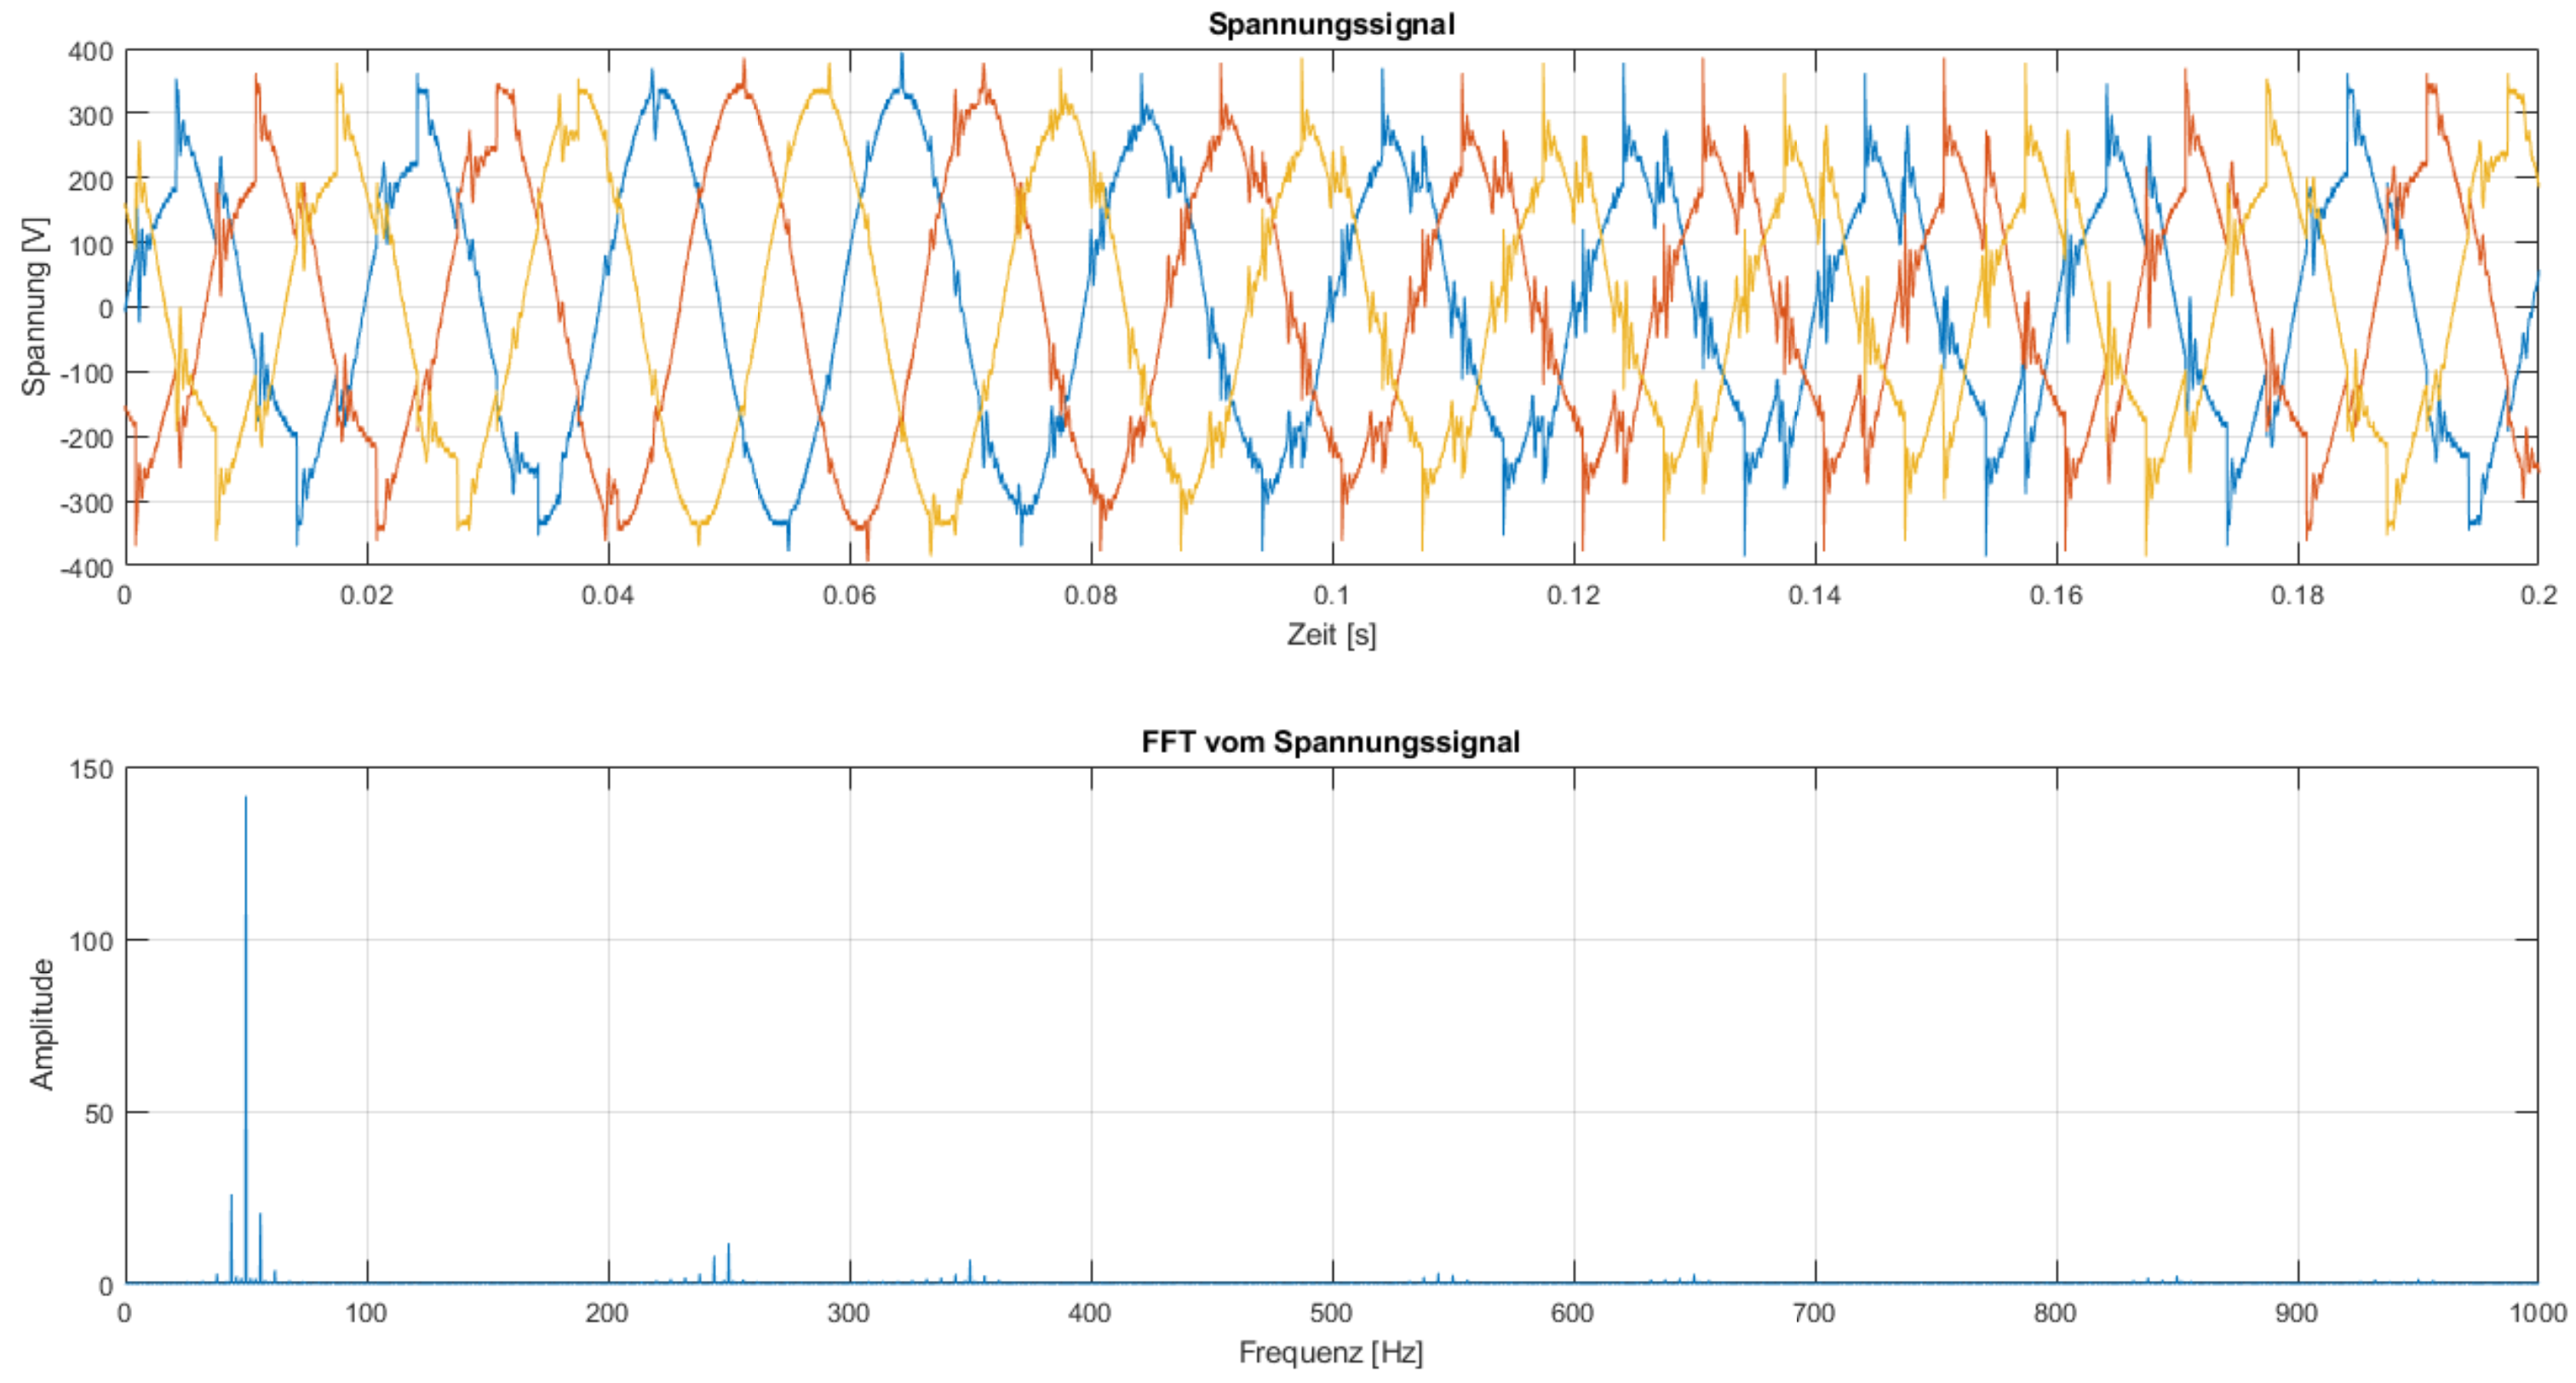
\includegraphics[width=\textwidth]{Messung_ASM_Phas_90grad.png}	
	\caption{Messung mit Phasenanschnitt 90\textdegree}\label{fig:Mess_ASM_Phas90}
\end{figure}

\newpage
\subsubsection*{Schwingungspaket 50\%}
\begin{figure}[ht!]
	\centering
	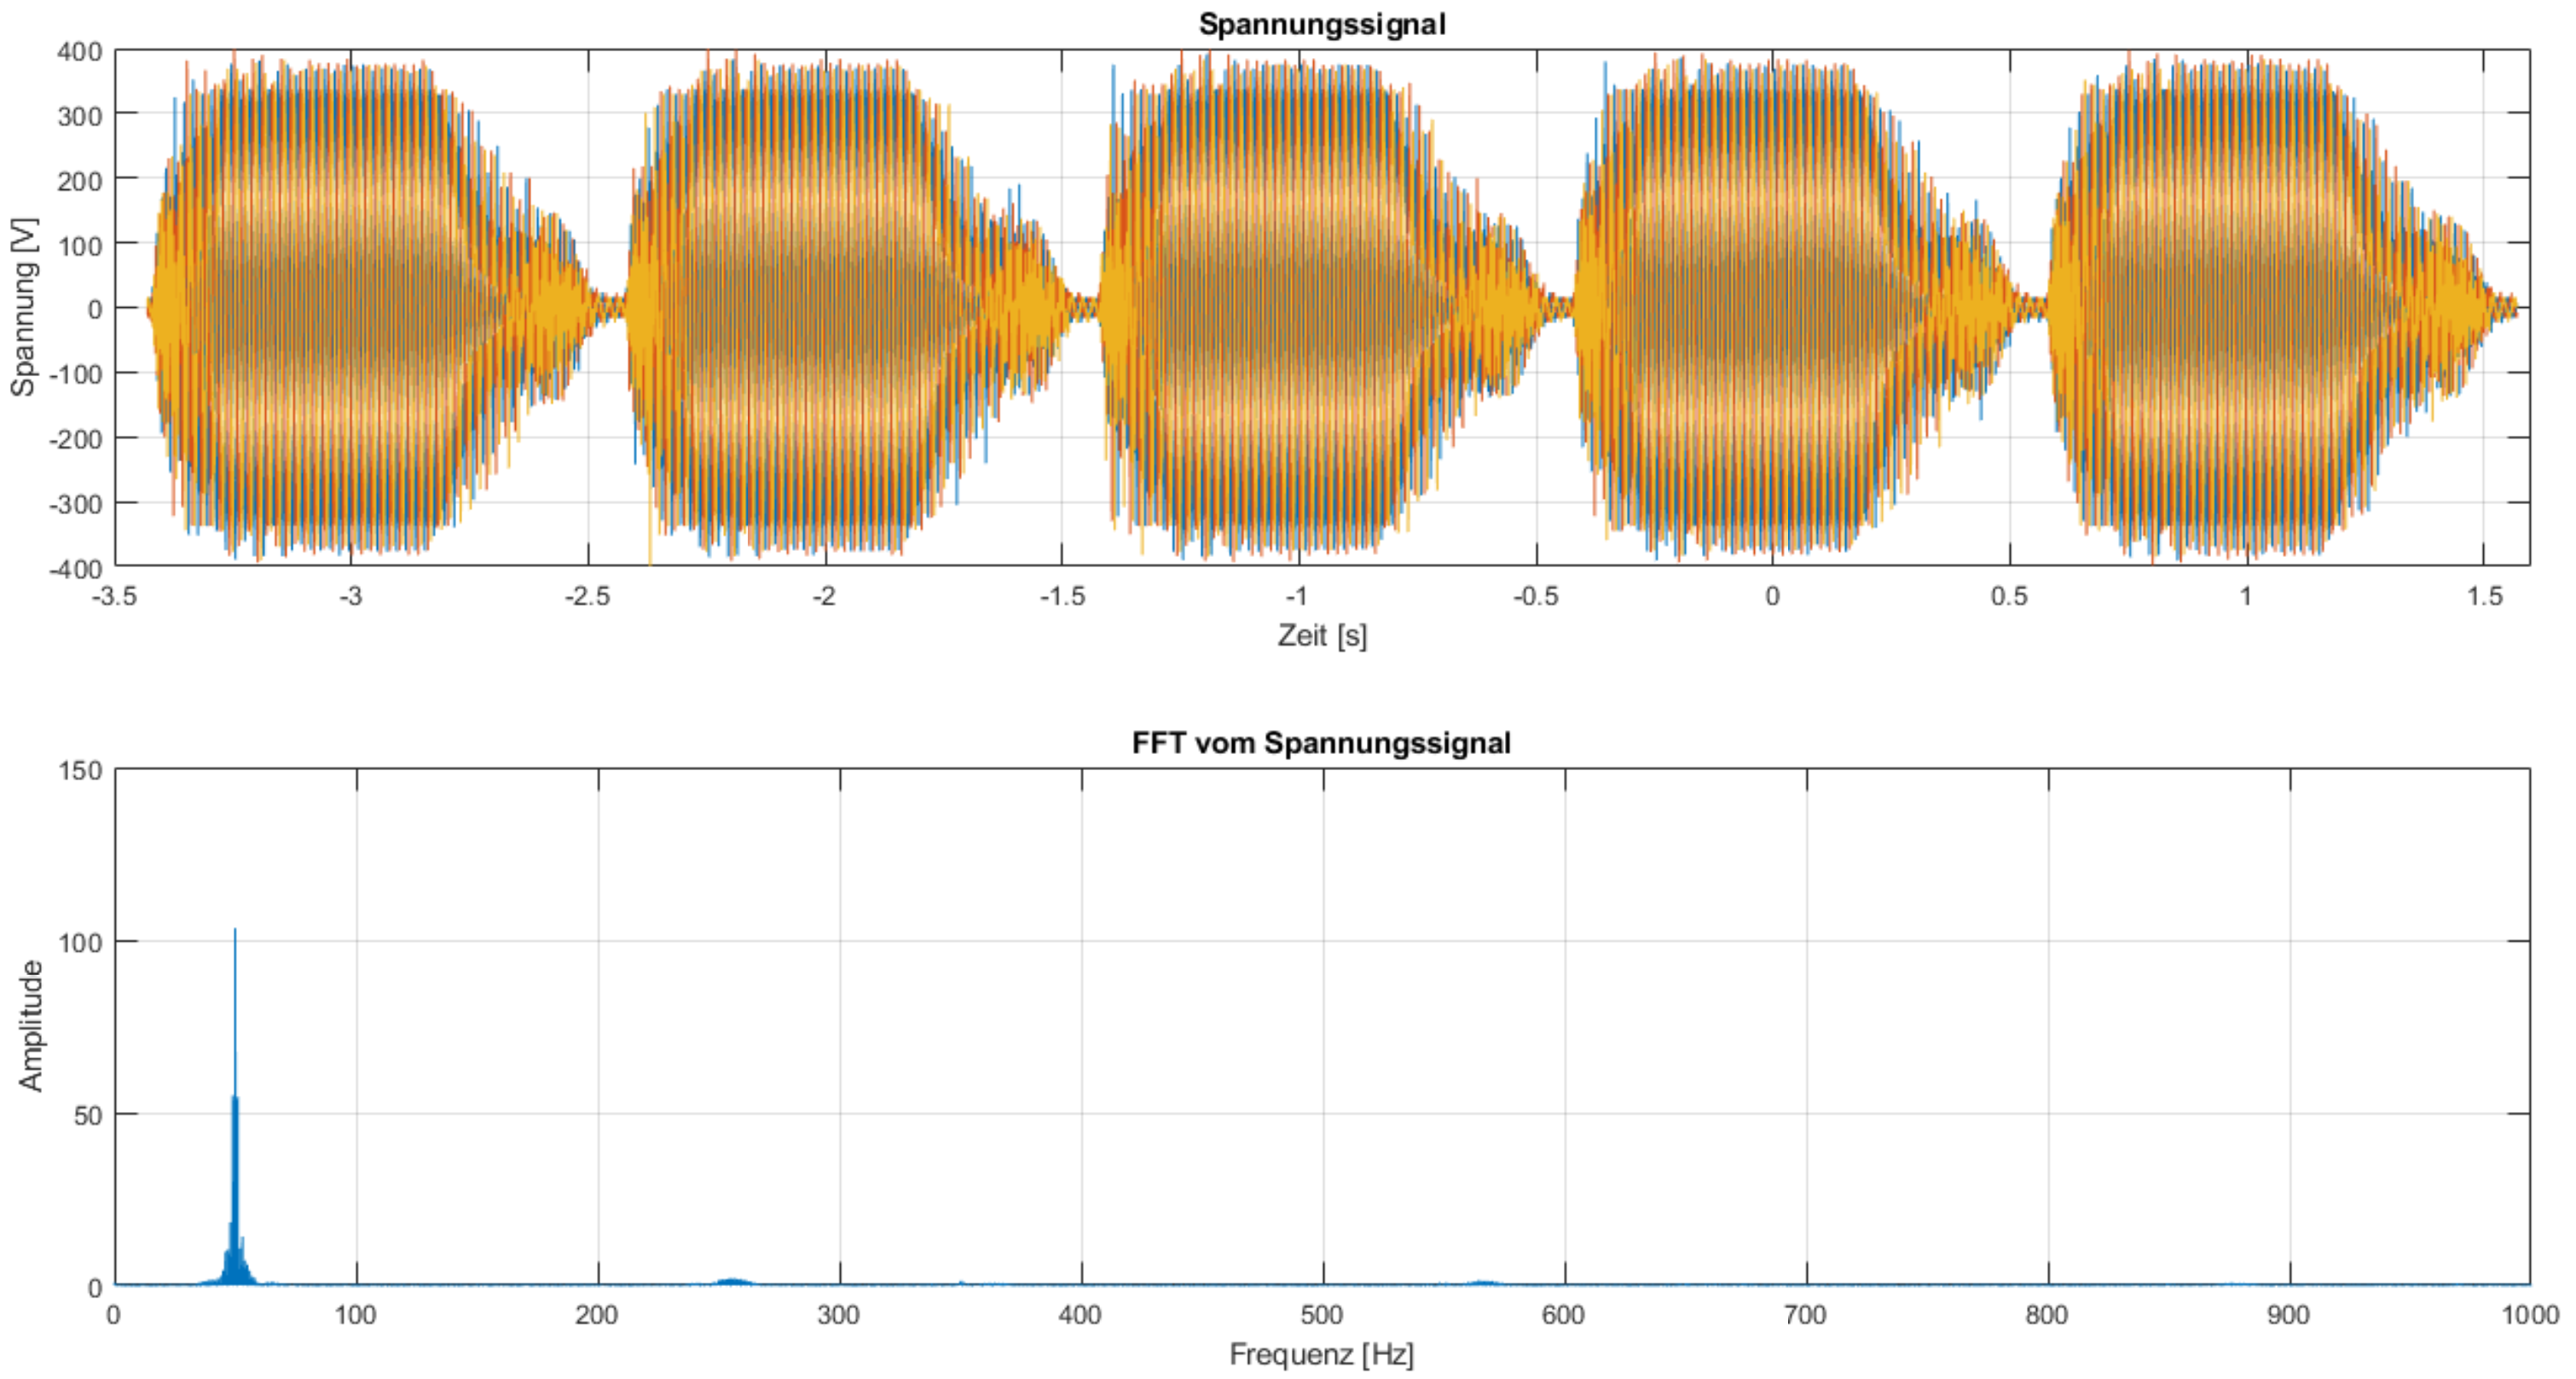
\includegraphics[width=\textwidth]{Messung_ASM_Schwing_0_5.png}	
	\caption{Messung mit Schwingungspaket 50\%}\label{fig:Mess_ASM_Schwing_0_5}
\end{figure}

\newpage
\subsubsection*{Schwingungspaket 80\%}
\begin{figure}[ht!]
	\centering
	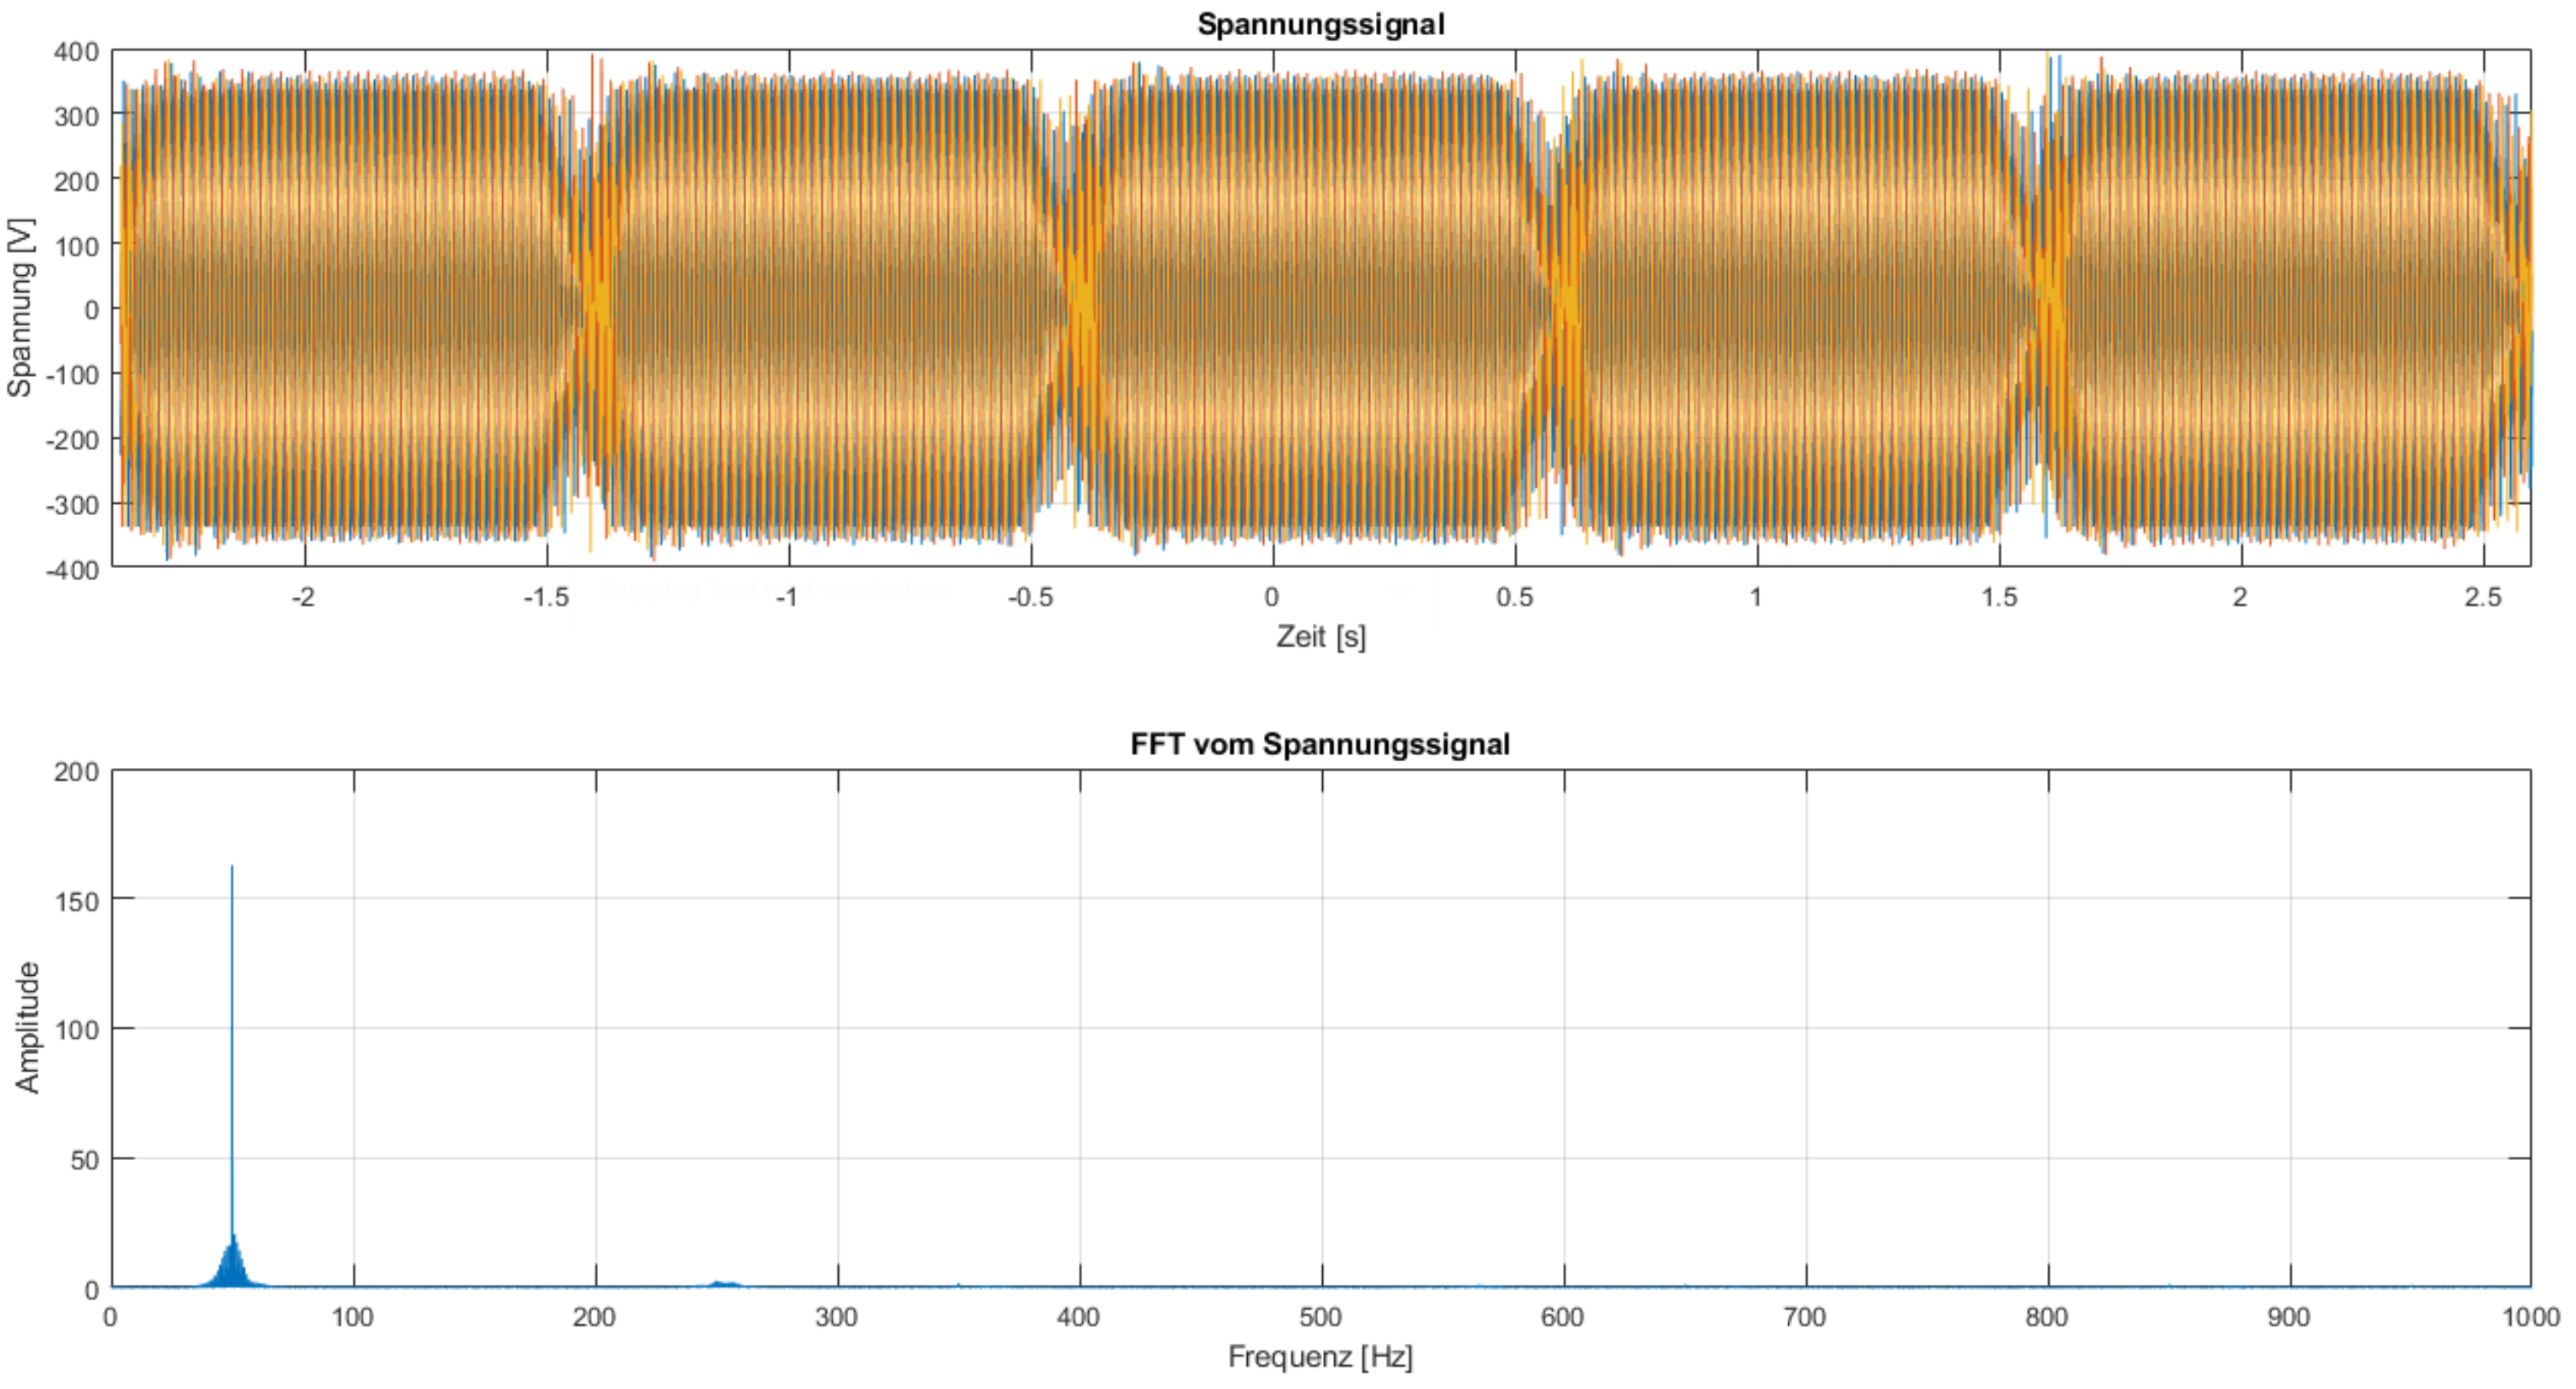
\includegraphics[width=\textwidth]{Messung_ASM_Schwing_0_8.png}	
	\caption{Messung mit Schwingungspaket 80\%}\label{fig:Mess_ASM_Schwing_0_8}
\end{figure}

\newpage
\subsubsection*{Sanft-Anlasser}
\begin{figure}[ht!]
	\centering
	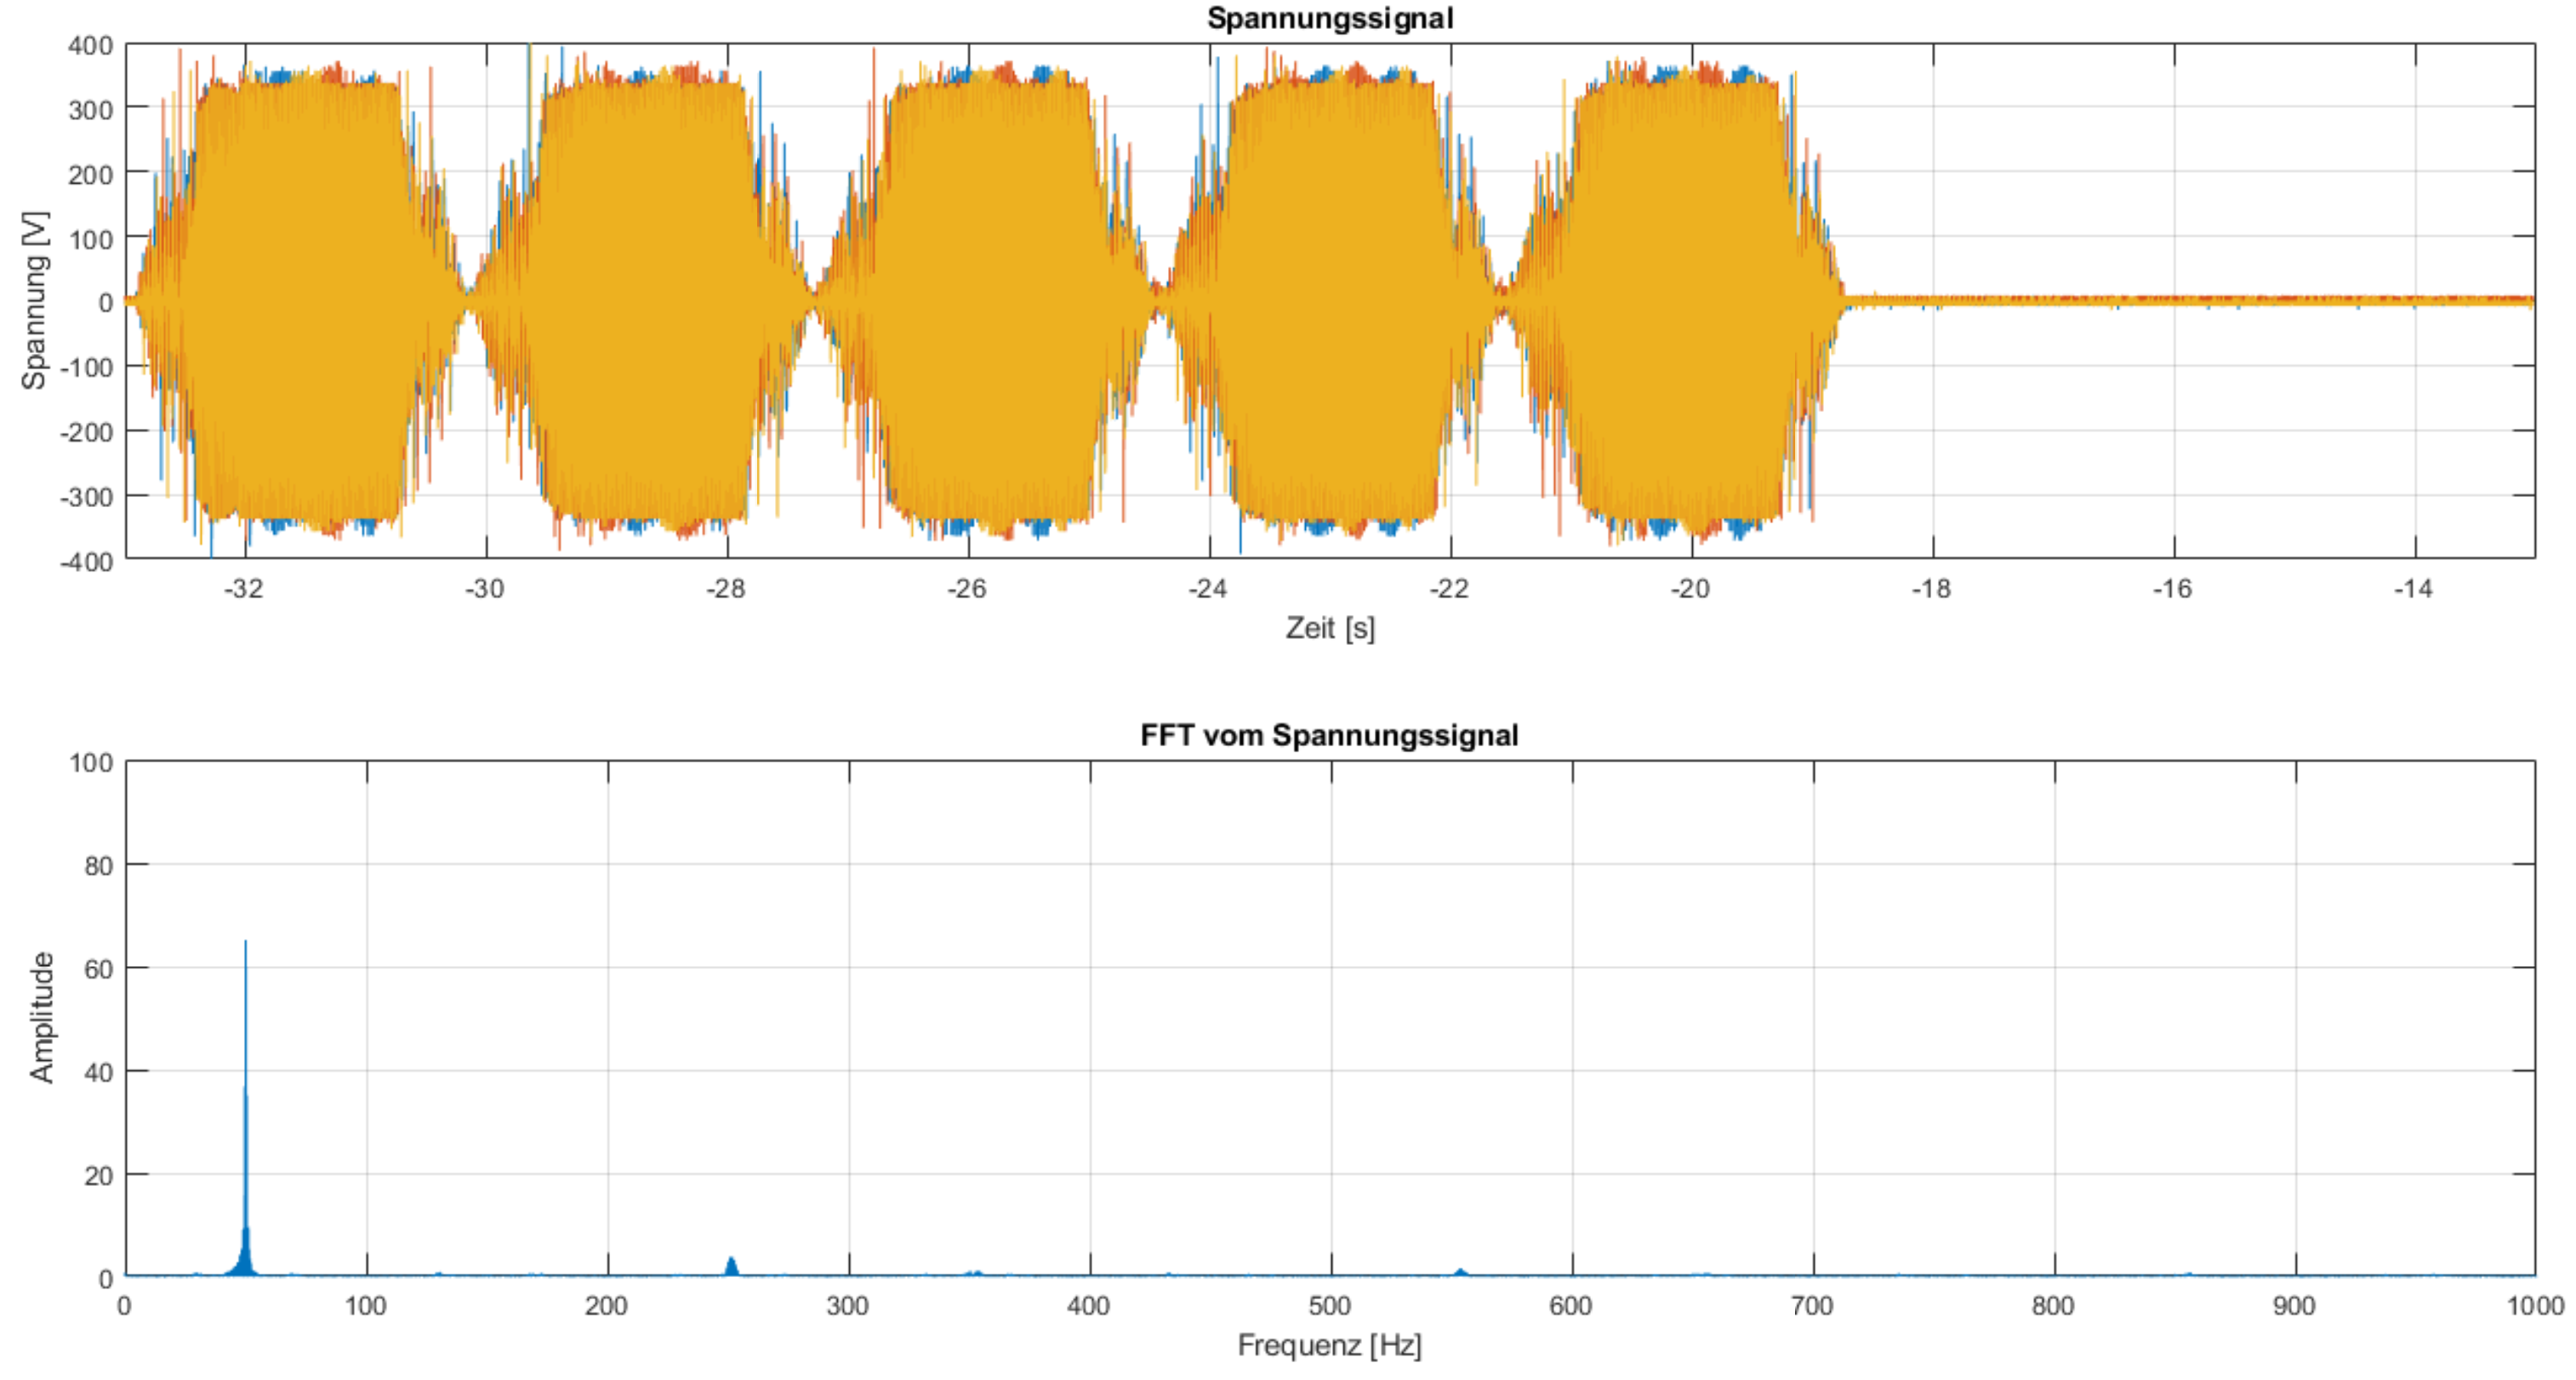
\includegraphics[width=\textwidth]{Messung_ASM_Sanft.png}	
	\caption{Messung mit Sanft Anlasser}\label{fig:Mess_ASM_Sanft}
\end{figure}

\newpage
\subsubsection*{Sanft-Anlasser Langsam}
\begin{figure}[ht!]
	\centering
	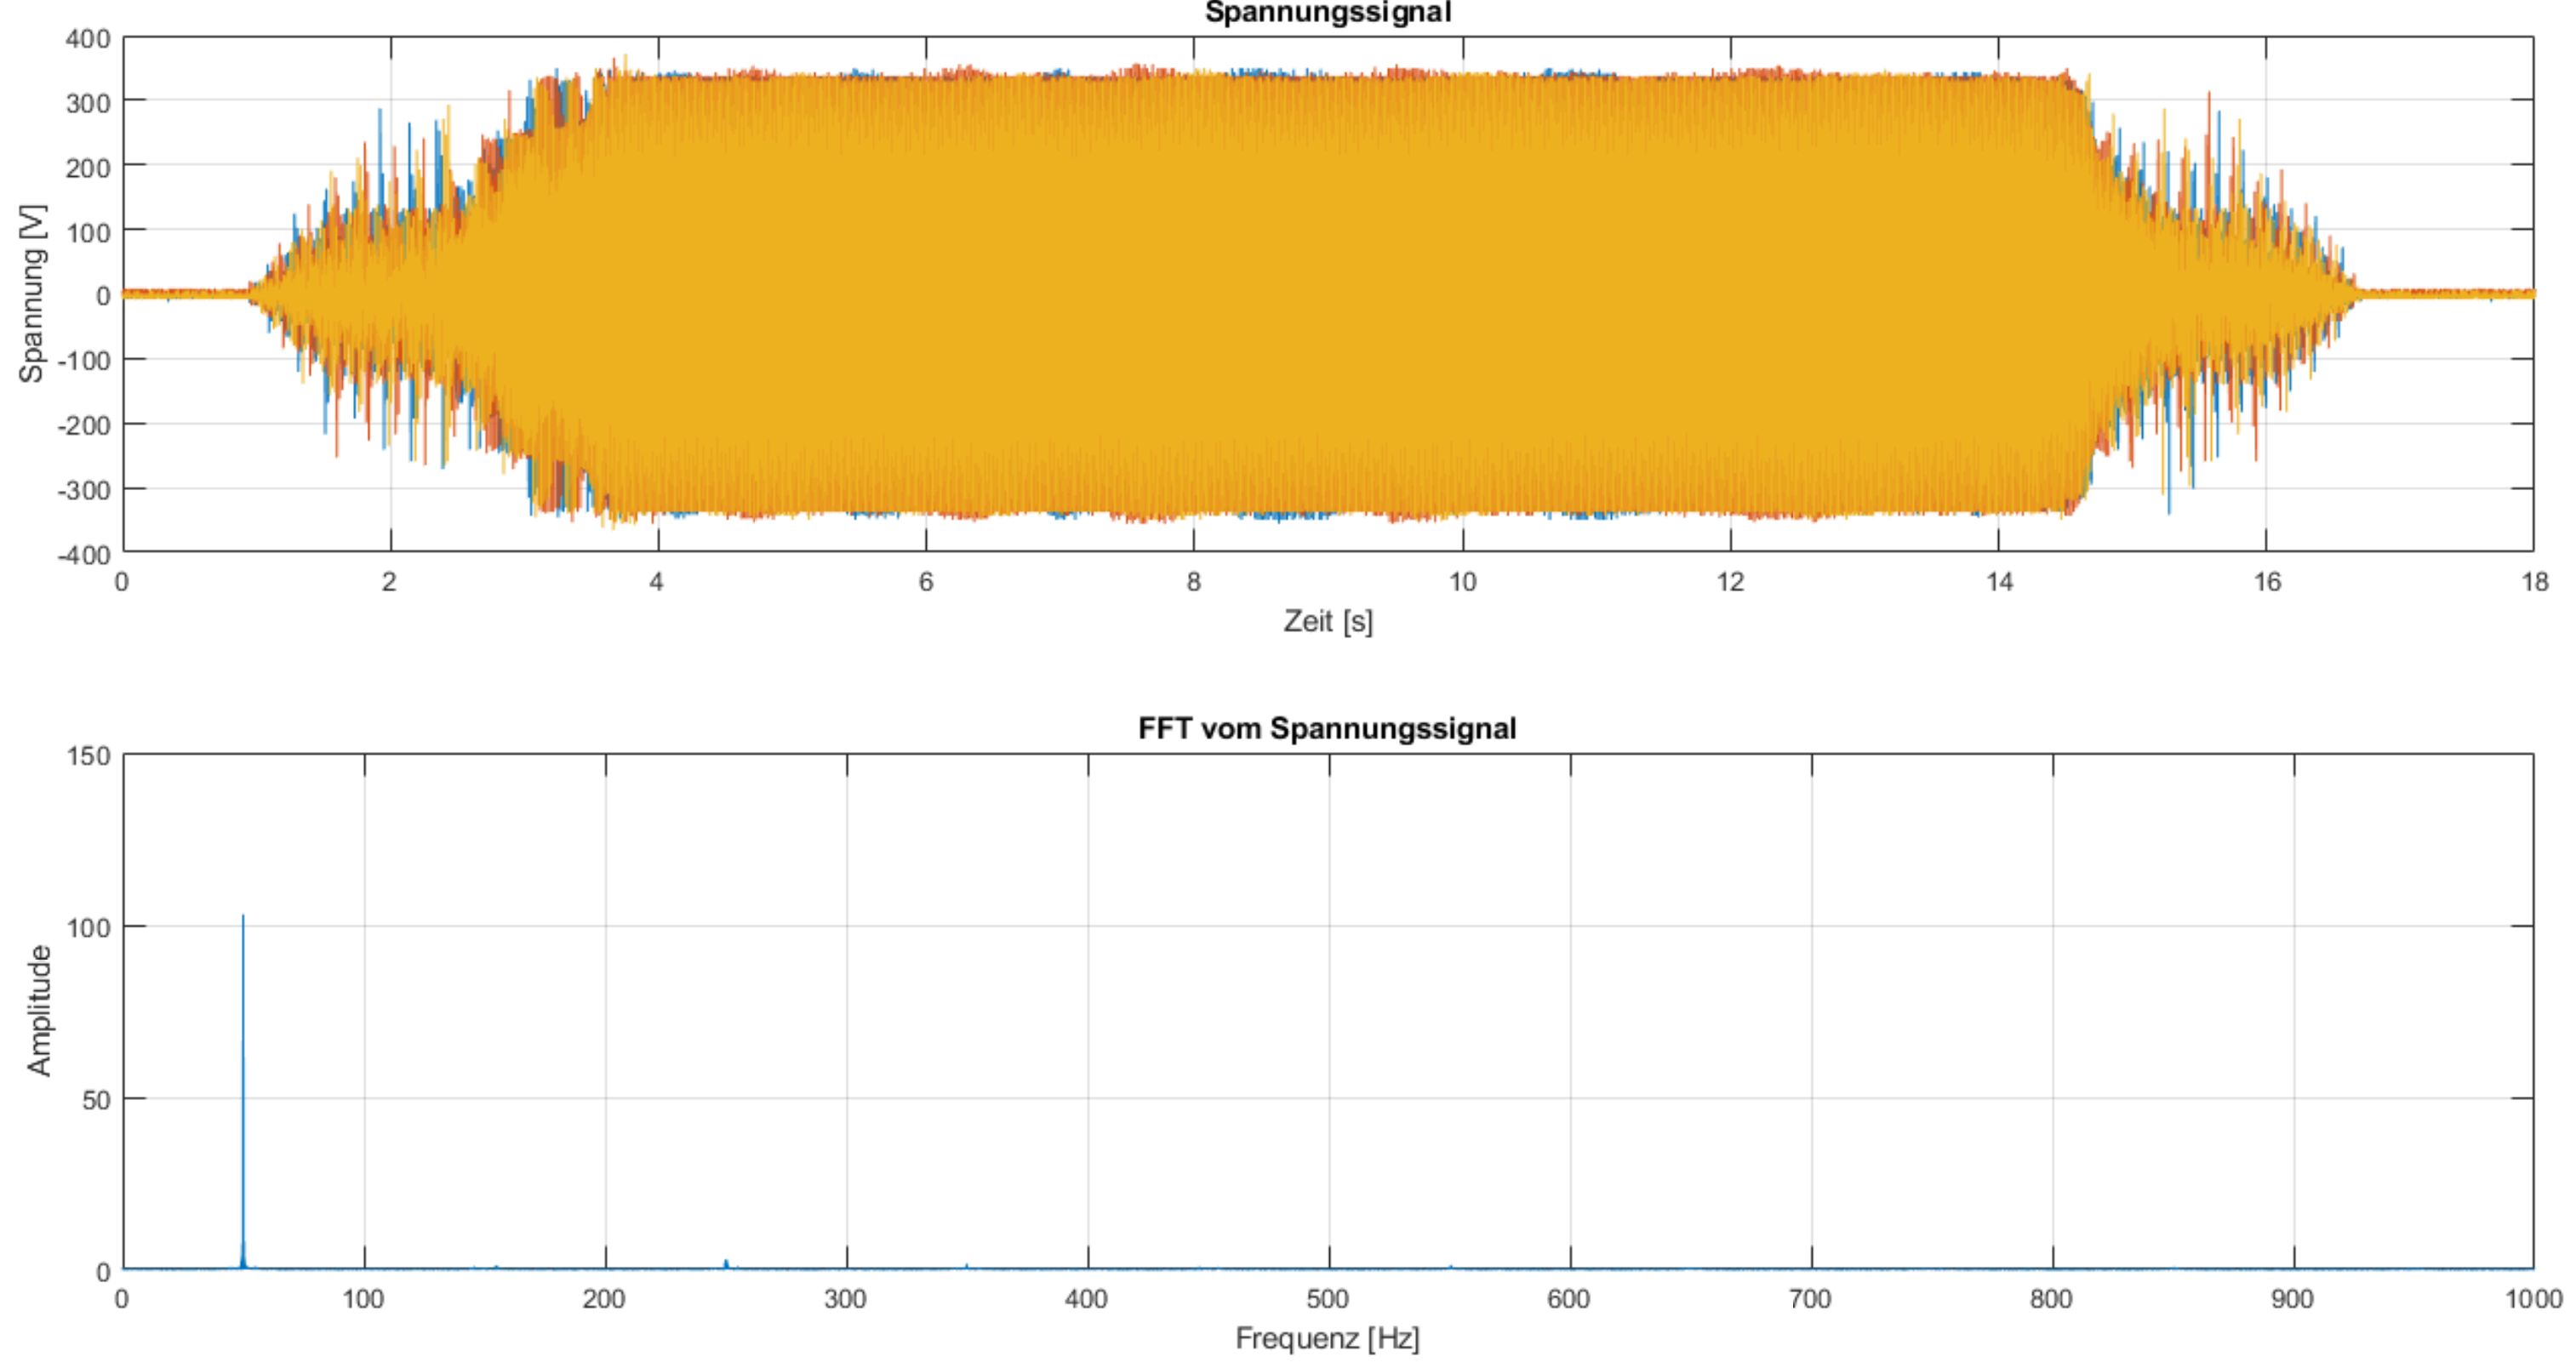
\includegraphics[width=\textwidth]{Messung_ASM_Sanft_langsam.png}	
	\caption{Messung mit Sanft-Anlasser langsam}\label{fig:Mess_ASM_Sanft_langsam}
\end{figure}

\newpage
\subsection{Messungen Ströme}
Um die Messungen mit den Normen vergleichen zu können, wurden die Ströme bei den verschiedenen Ansteuerungsarten gemessen. Da aber durch den Widerstand keine \SI{16}{A} Effektivstrom durchgelassen werden können, da der Widerstand bei \SI{150}{\Omega} nur bis zu \SI{2.4}{A} verträgt, mussten die gemessenen Werte auf \SI{16}{A} hochgerechnet werden.
Von den berechneten Werten kann das FFT mit Matlab gemacht werden und die Amplituden mit den Normen verglichen werden. Dazu wurden die Werte des FFTs in eine Tabelle aufgetragen.
\subsubsection{Messungen Widerstand}


\subsubsection*{Phasenanschnitt 60\textdegree}

\begin{figure}[ht!]
	\centering
	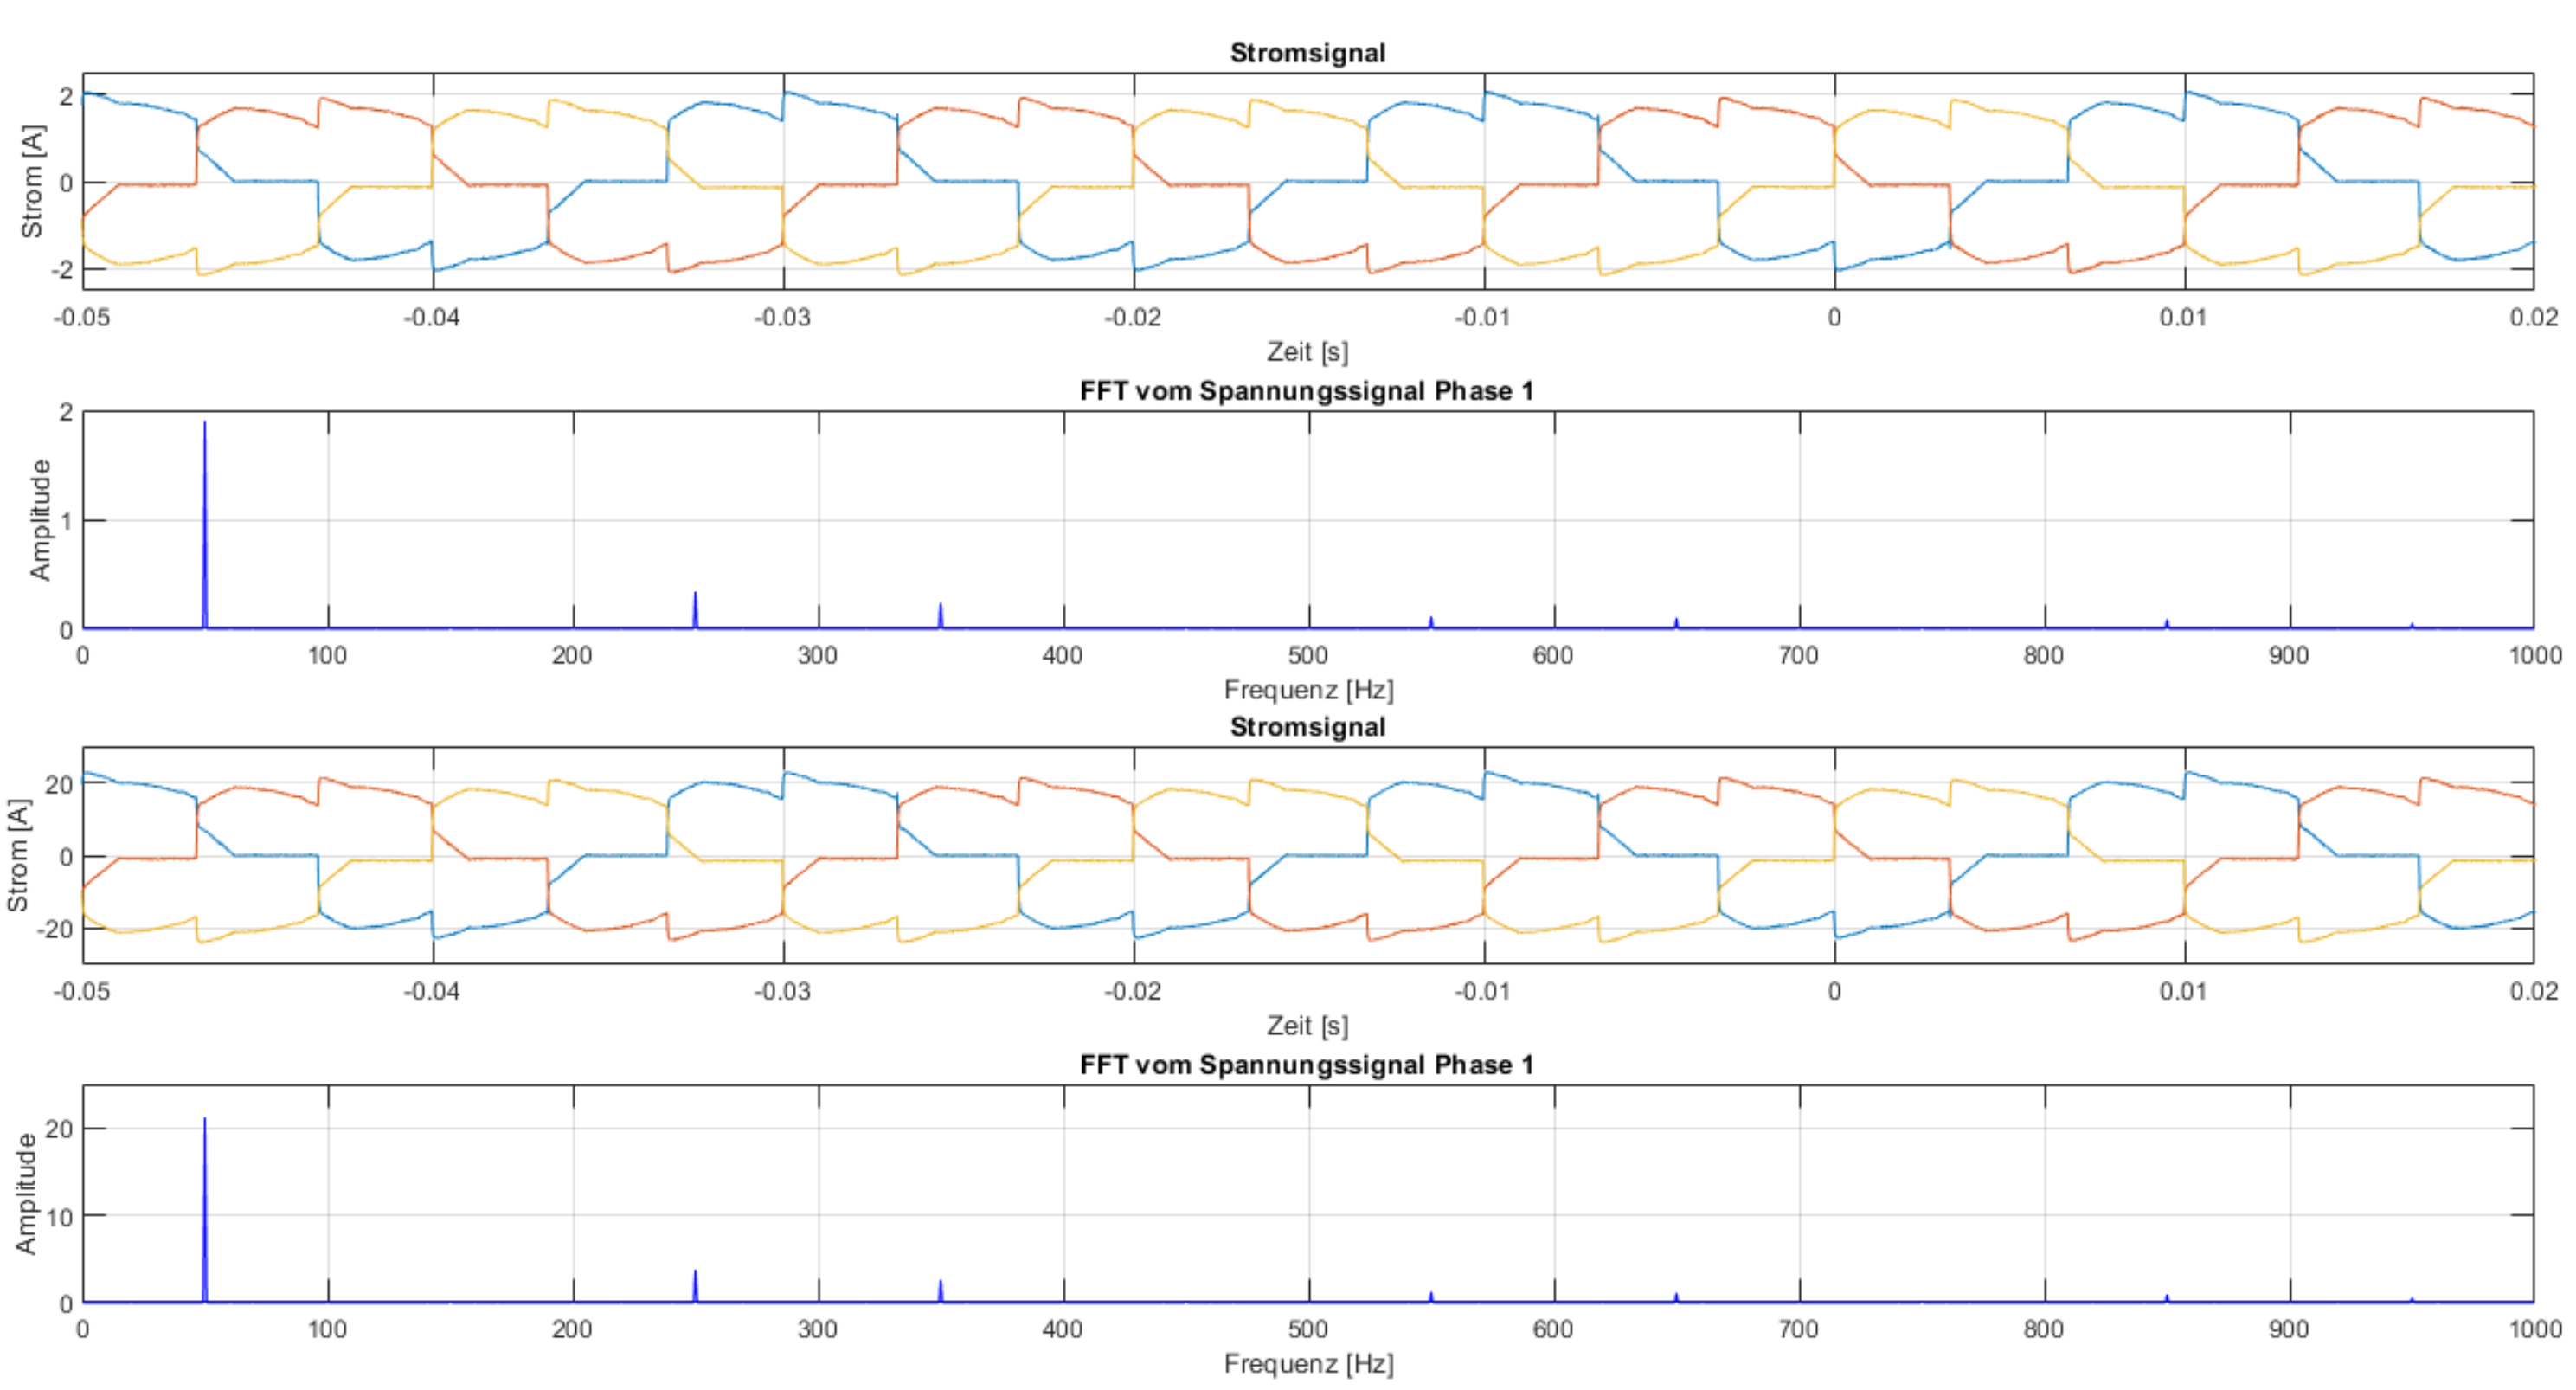
\includegraphics[width=\textwidth]{Messung_Widerstand_Phas_60grad_stroeme.png}	
	\caption{Messung mit Phasenanschnitt 60\textdegree}\label{fig:Mess_Widerstand_Phas_60grad_stroeme}
\end{figure}

\begin{table}[ht!]
	\centering
	\begin{tabular}{|l|l|}
		\hline
		Oberschwingungsordnung & Amplitude \\ \hline
		1                      & 21.1996   \\ \hline
		5                      & 3.7851    \\ \hline
		7                      & 2.6127    \\ \hline
		11                     & 1.2267    \\ \hline
		13                     & 1.0988    \\ \hline
		17                     & 0.9366    \\ \hline
		19                     & 0.7342    \\ \hline
	\end{tabular}
\caption{Amplitudenwerte bei den harmonischen Oberschwingungen bei Phasenanschnitt 60\textdegree}\label{tab:Phas_60_Stroeme}
\end{table}


\newpage
\subsubsection*{Phasenanschnitt 90\textdegree}
\begin{figure}[ht!]
	\centering
	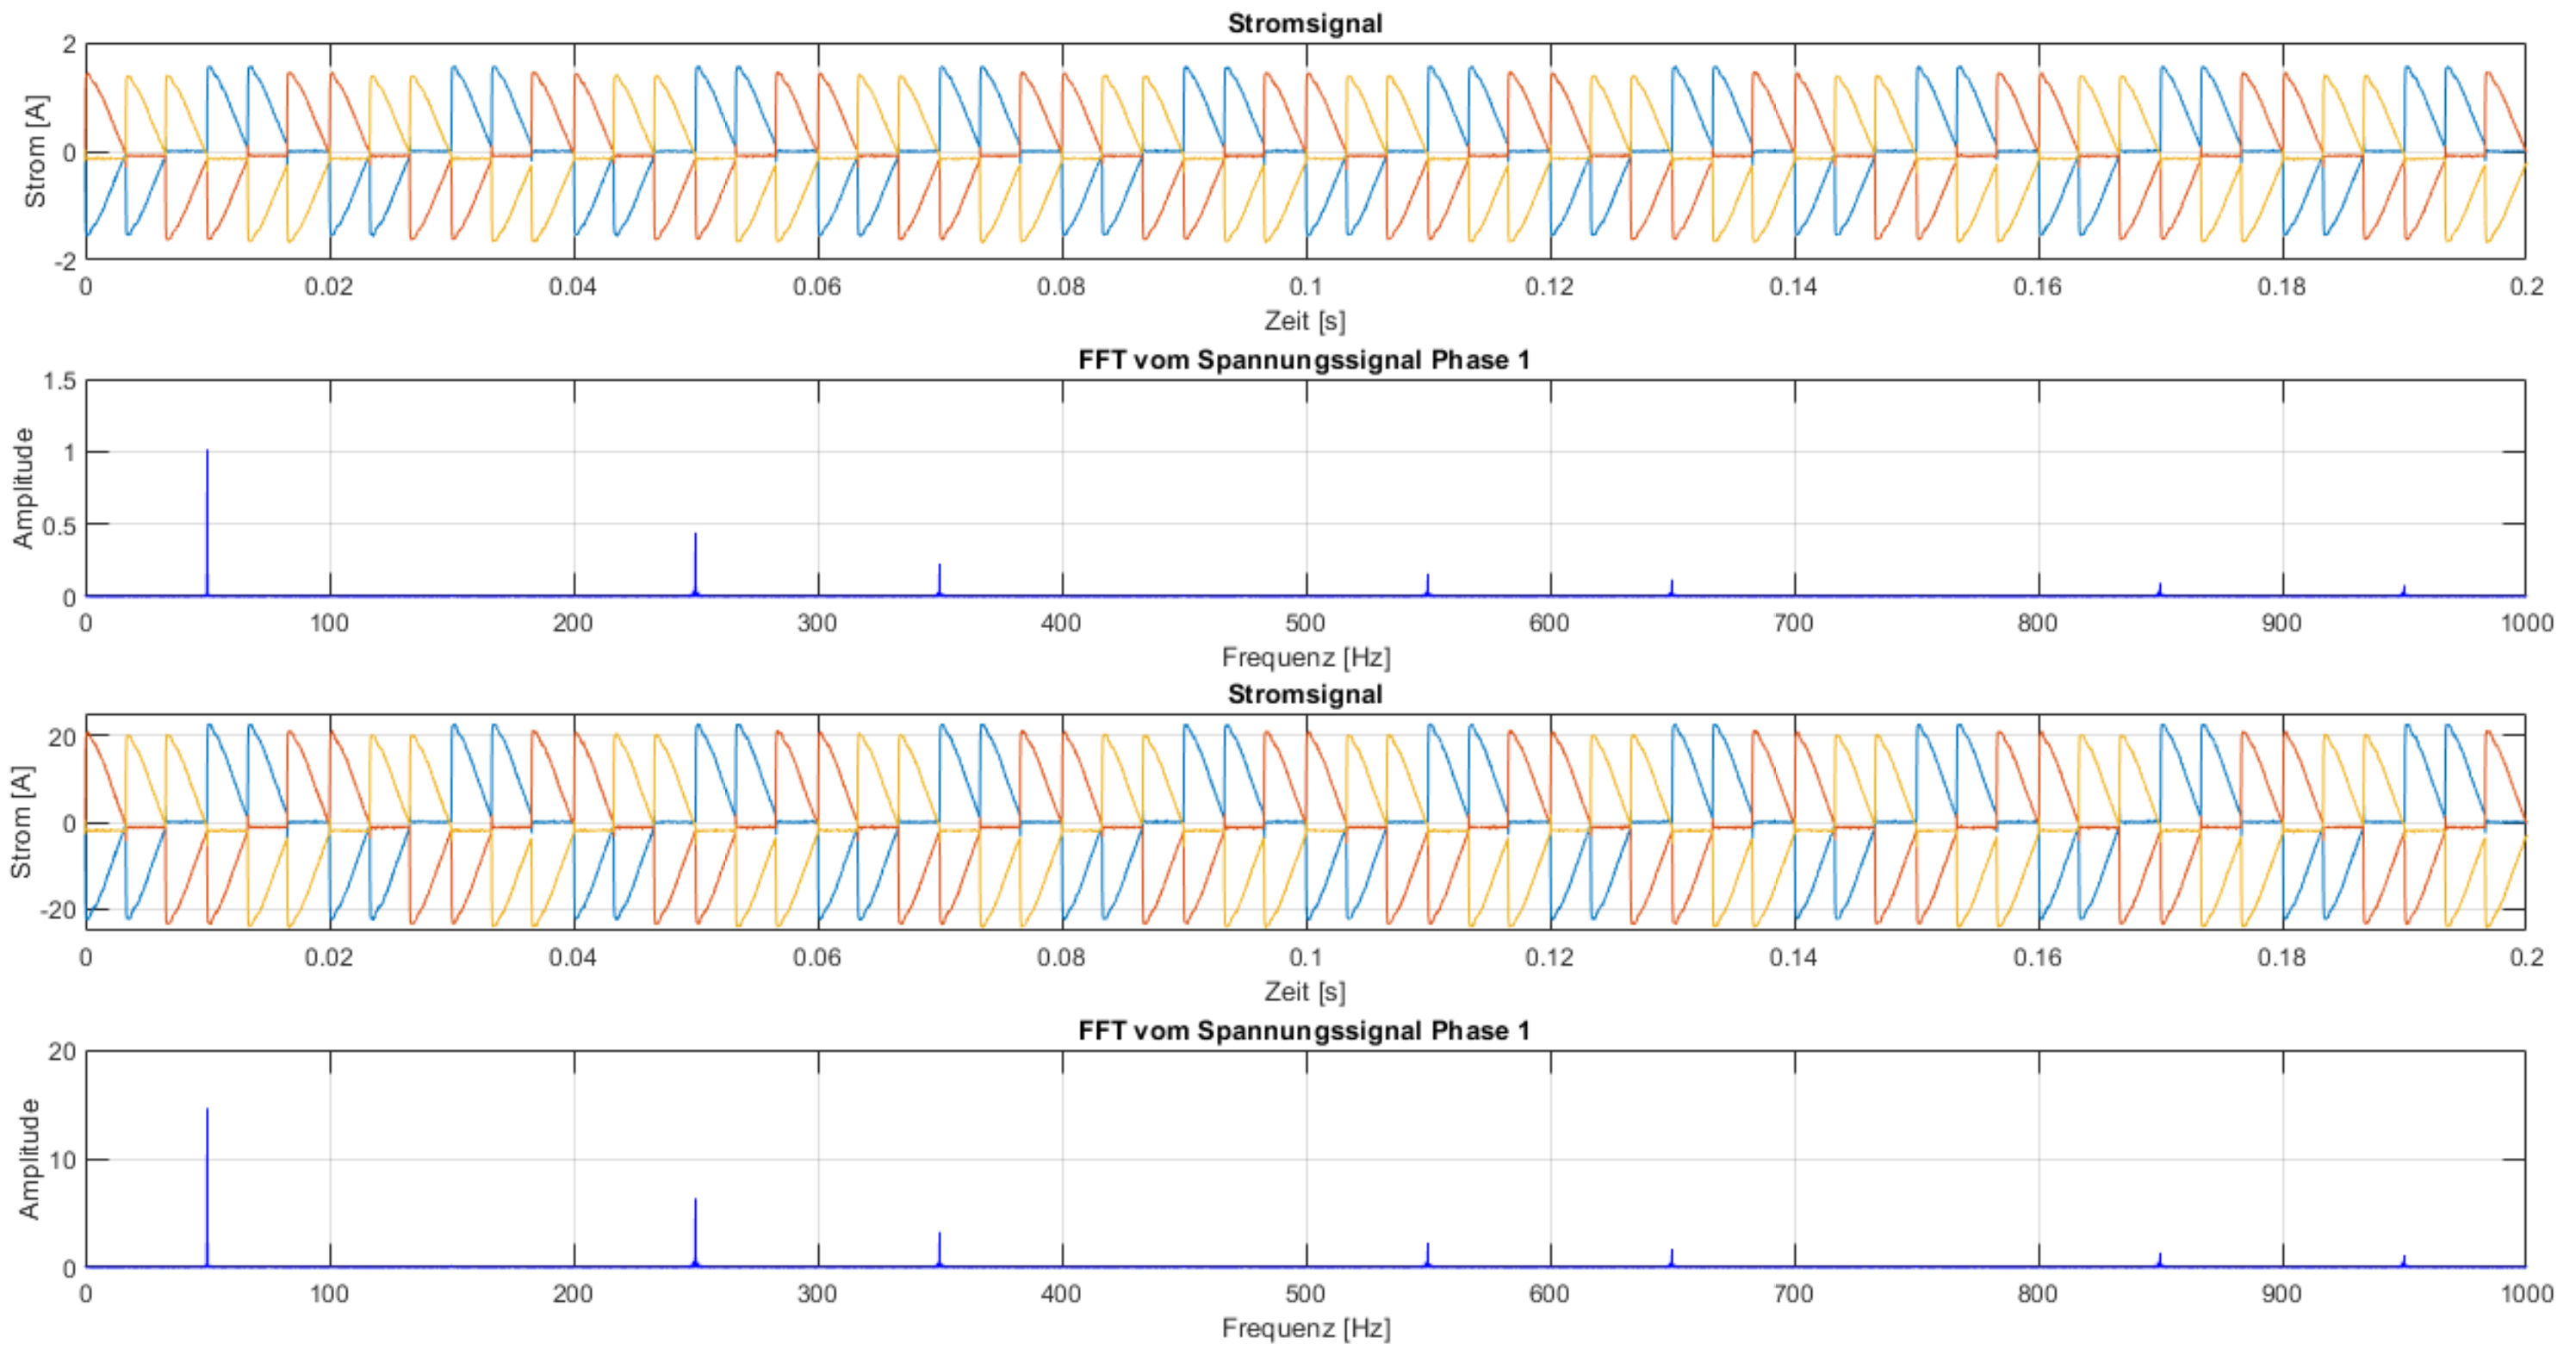
\includegraphics[width=\textwidth]{Messung_Widerstand_Phas_90grad_stroeme.png}	
	\caption{Phasenanschnitt 90\textdegree}\label{fig:Mess_Widerstand_Phas_90grad_stroeme}
\end{figure}

\begin{table}[ht!]
	\centering
	\begin{tabular}{|l|l|}
		\hline
		Oberschwingungsordnung & Amplitude [A] \\ \hline
		1       & 14.6470   \\ \hline
		5      & 6.3481    \\ \hline
		7      & 3.2571    \\ \hline
		11      & 2.2730    \\ \hline
		13      & 1.6960    \\ \hline
		17      & 1.3474    \\ \hline
		19      & 1.1247    \\ \hline
	\end{tabular}
	\caption{Amplitudenwerte bei den harmonischen Oberschwingungen bei Phasenanschnitt 90\textdegree}\label{tab:Phas_90_Stroeme}
\end{table}
Wenn die Werte mit der Werte der Tabelle \ref{tab:Grenzwerte_Normen} verglichen werden, ist ersichtlich, dass die Amplituden bei der Oberschwingungsordung 5 bis 19 zu hoch sind. So kann gesagt werden, dass sich der Phasenanschnitt mit 90\textdegree \hspace{0.02cm} nicht eignet um Widerstände anzusteuern, da diese nicht den Normen entsprechen. Auf der Abbildung \ref{fig:Mess_Widerstand_Phas_90grad_stroeme} ist ersichtlich, dass bei den Oberschwingungsordnungen 3, 9 und 15 die Amplitude 0 ist, deswegen wurde diese nicht in der Tabelle \ref{tab:Phas_60_Stroeme} aufgeführt.


\newpage
\subsubsection*{Sanft-Anlasser}
\begin{figure}[ht!]
	\centering
	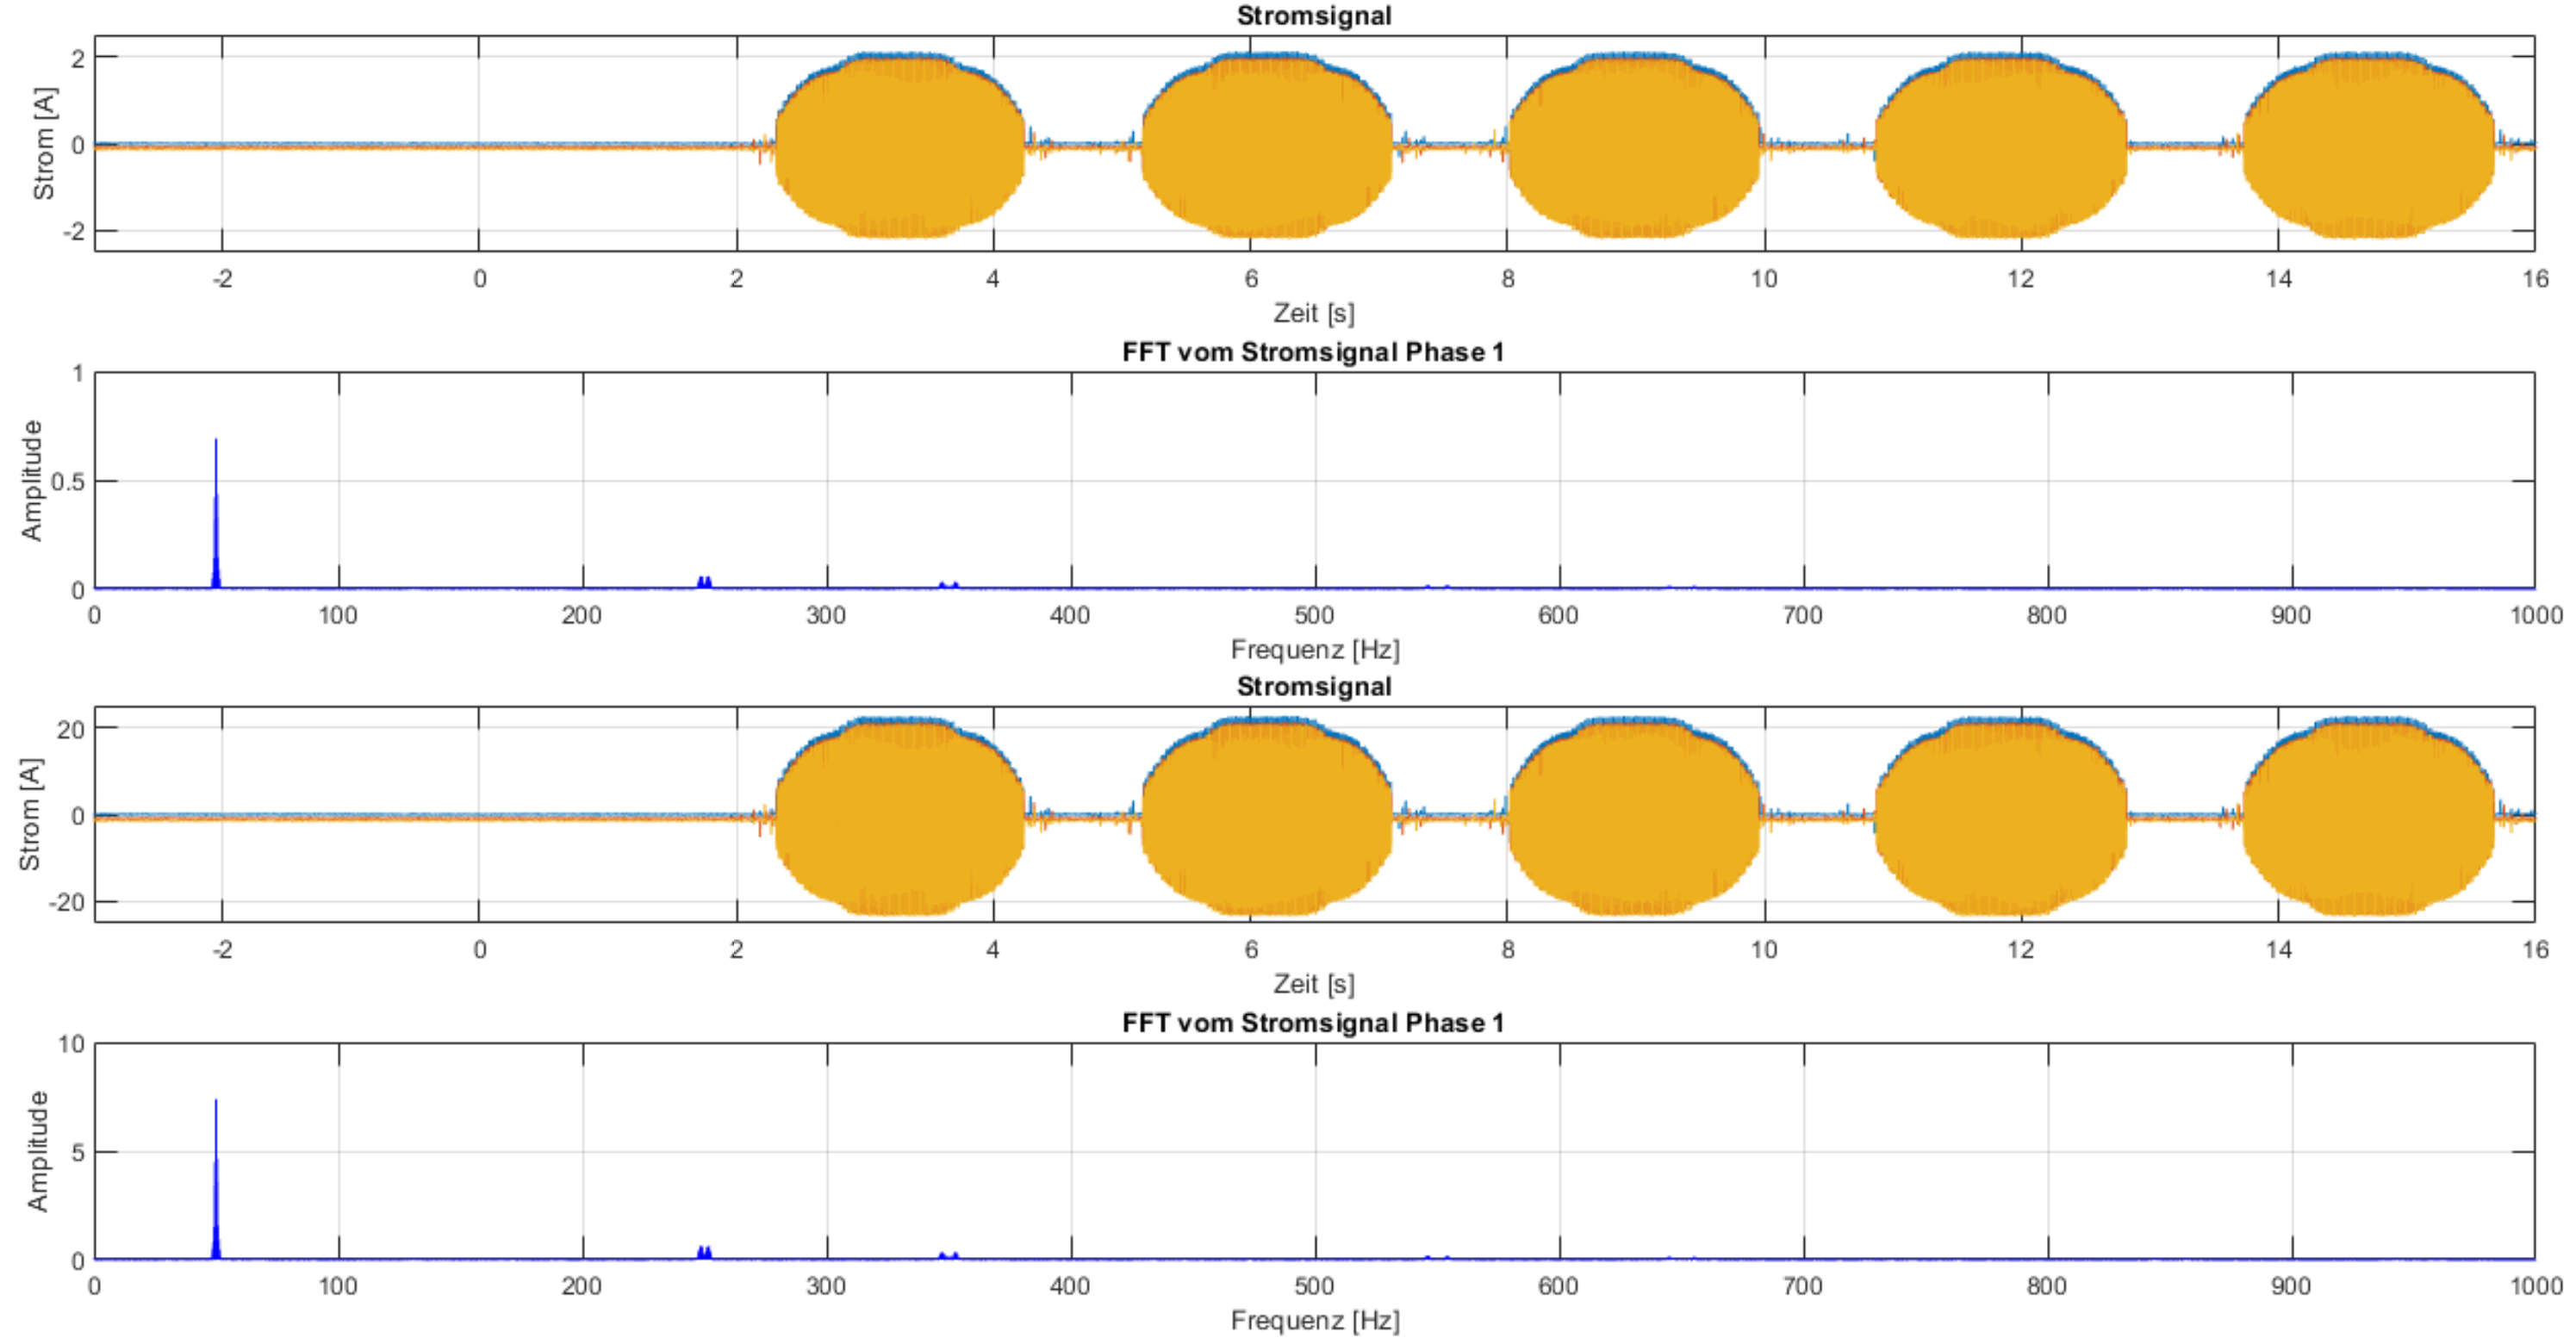
\includegraphics[width=\textwidth]{Messung_Widerstand_Sanft_stroeme.png}	
	\caption{Messung mit Sanft-Anlasser}\label{fig:Mess_Widerstand_Sanft_stroeme}
\end{figure}
Da beim Sanft-Anlasser ab der fünften Harmonischen die Amplitude unter \SI{0.3}{A} sind, wurde bei dieser Messung auf eine Tabelle mit den Oberschwingungen verzichtet. Jedoch sind bei dieser Messung die Sub- und Zwischenharmonische sehr interessant. 

\begin{table}[ht!]
	\centering
	\begin{tabular}{|l|l|}
		\hline
		Frequenz {[}Hz{]} & Amplitude {[}A{]} \\ \hline
		49.3              & 1.5146            \\ \hline
		49.6              & 4.4853            \\ \hline
		49.7              & 2.618             \\ \hline
		50                & 7.3857            \\ \hline
		50.05             & 3.73              \\ \hline
		50.35             & 4.662             \\ \hline
		50.7              & 1.5504            \\ \hline
		248.65            & 0.6226            \\ \hline
		250               & 0.0883            \\ \hline
		251.45            & 0.6               \\ \hline
	\end{tabular}
	\caption{Amplitudenwerte bei den harmonischen Oberschwingungen bei Phasenanschnitt 90\textdegree}\label{tab:Sanft_stroeme}
\end{table}




\newpage
\subsubsection*{Sanft-Anlasser langsam}
\begin{figure}[ht!]
	\centering
	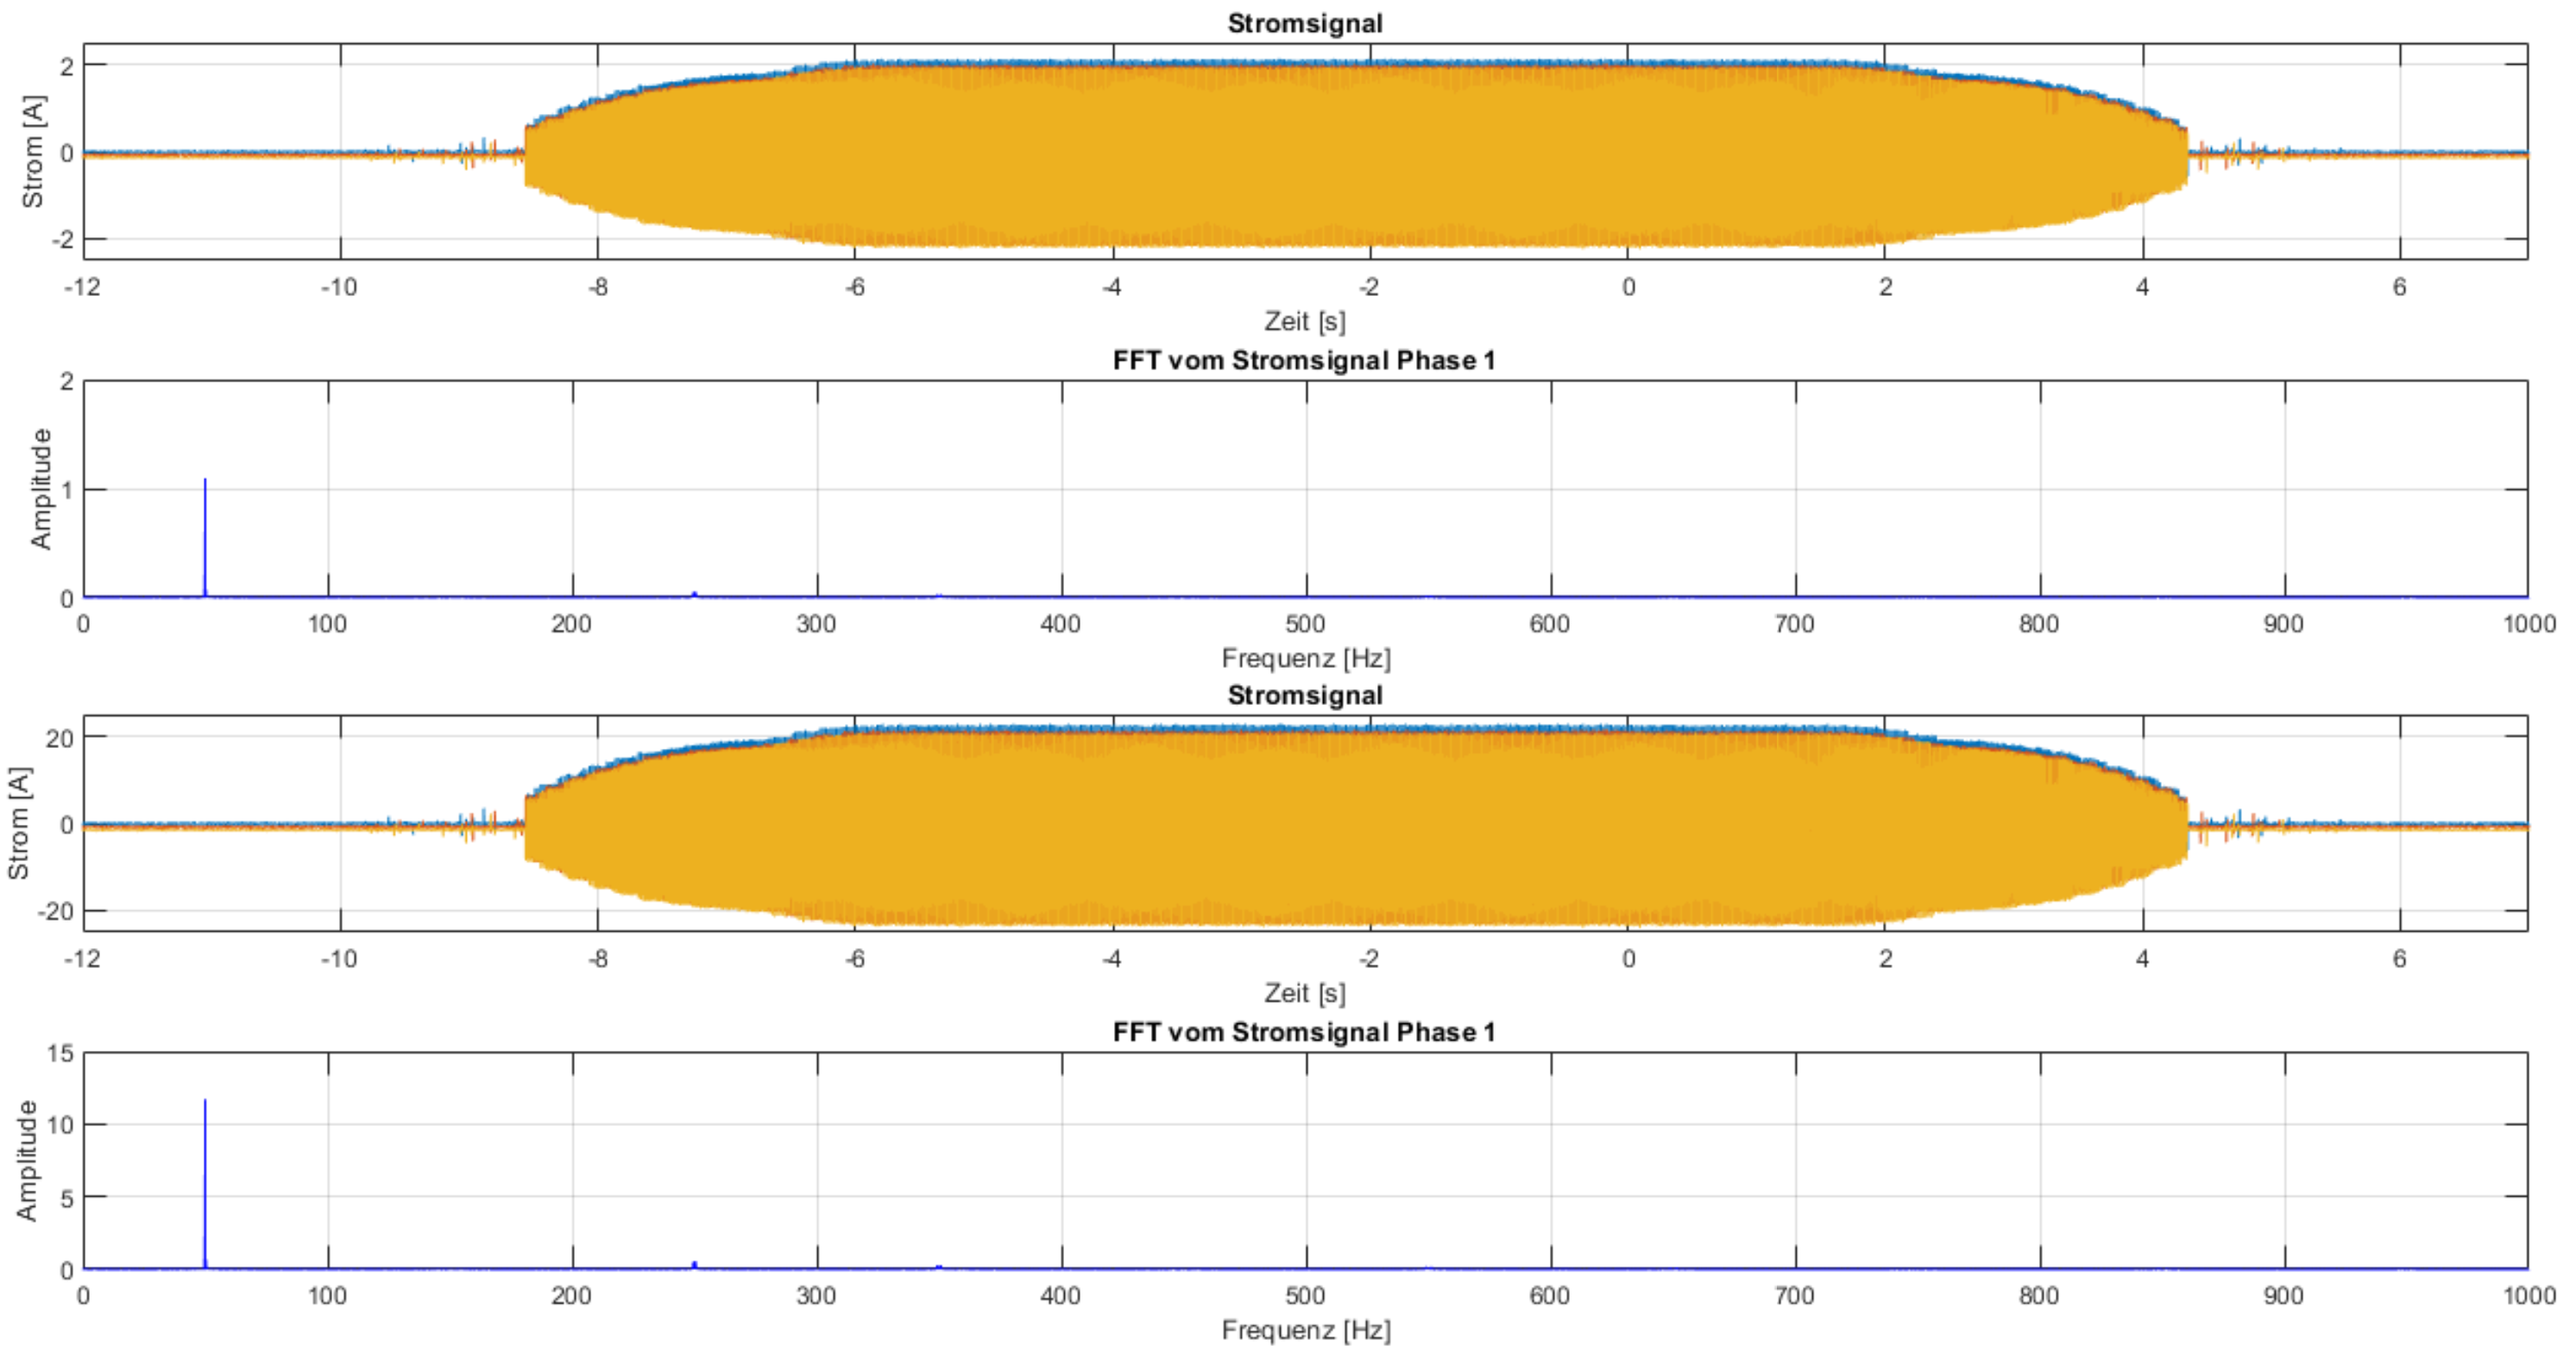
\includegraphics[width=\textwidth]{Messung_Widerstand_Sanft_langsam_stroeme.png}	
	\caption{Messung mit Sanft-Anlasser langsam}\label{fig:Mess_Widerstand_Sanft_langsam_stroeme}
\end{figure}


\newpage
\subsubsection{Messungen ASM}

\subsubsection*{Phasenaschnitt 60\textdegree}
\begin{figure}[ht!]
	\centering
	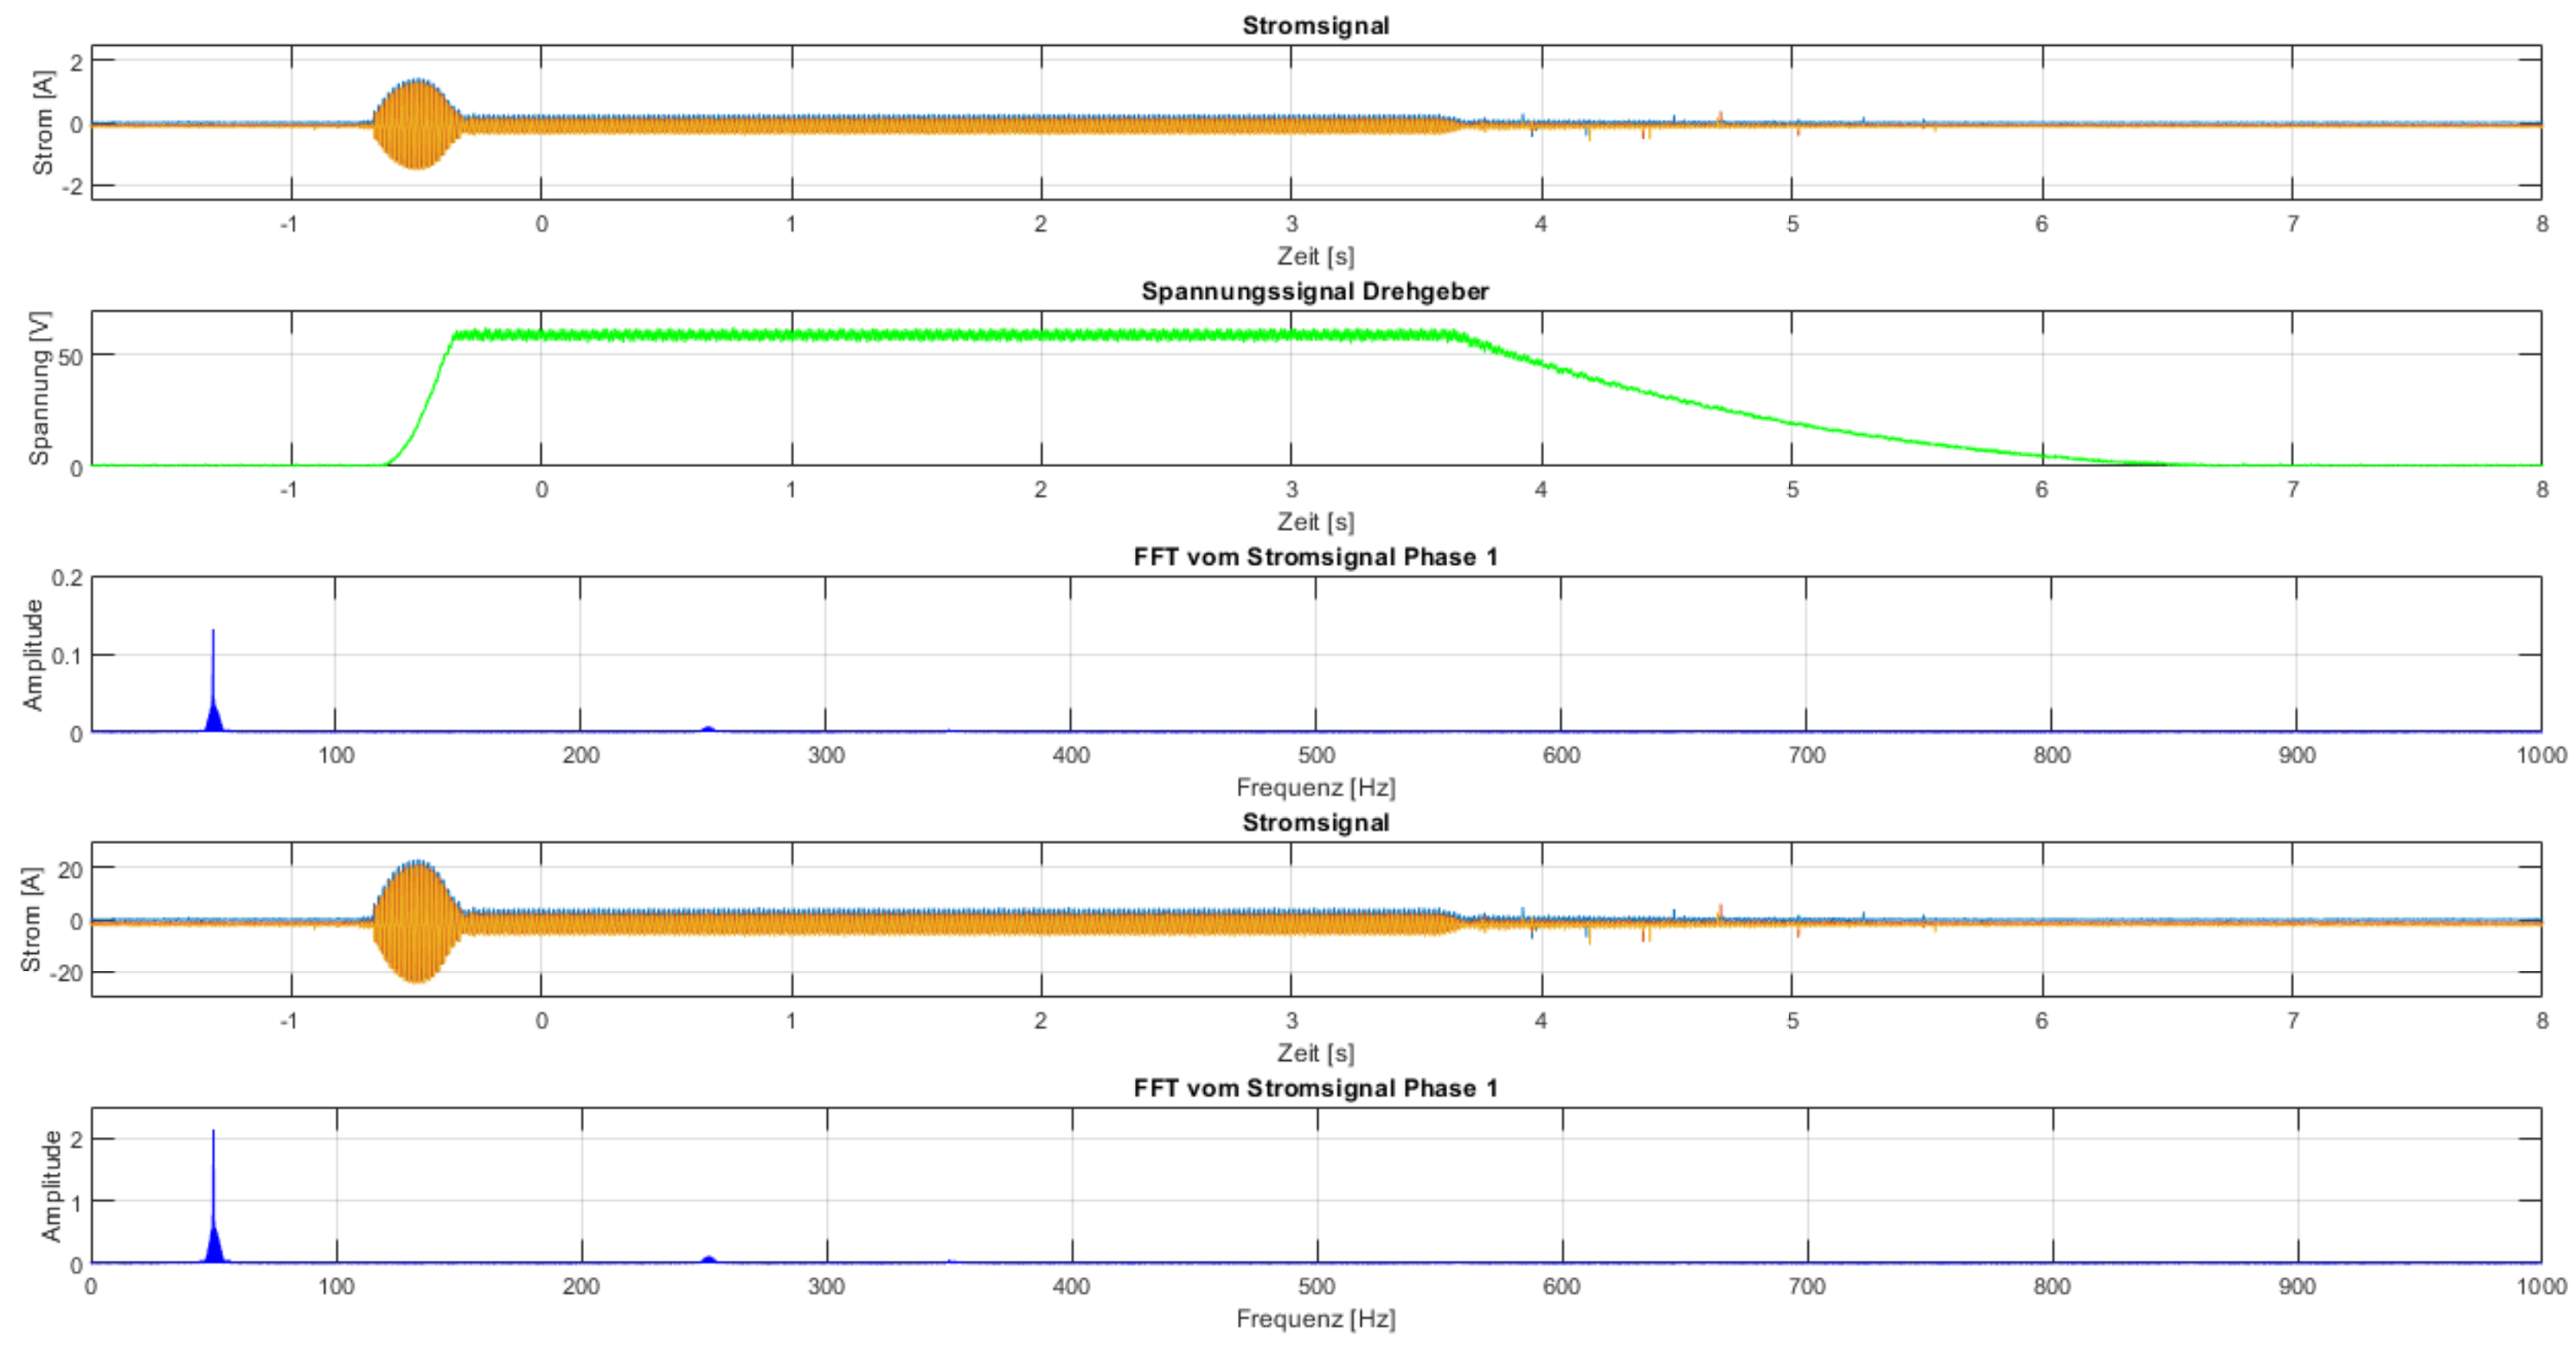
\includegraphics[width=\textwidth]{Messung_ASM_Phas_60grad_stroeme}	
	\caption{Messung mit Phasenanschnitt 60\textdegree}\label{fig:Mess_Phas_60grad_stroeme}
\end{figure}

\newpage
\subsubsection*{Phasenaschnitt 90\textdegree}
\begin{figure}[ht!]
	\centering
	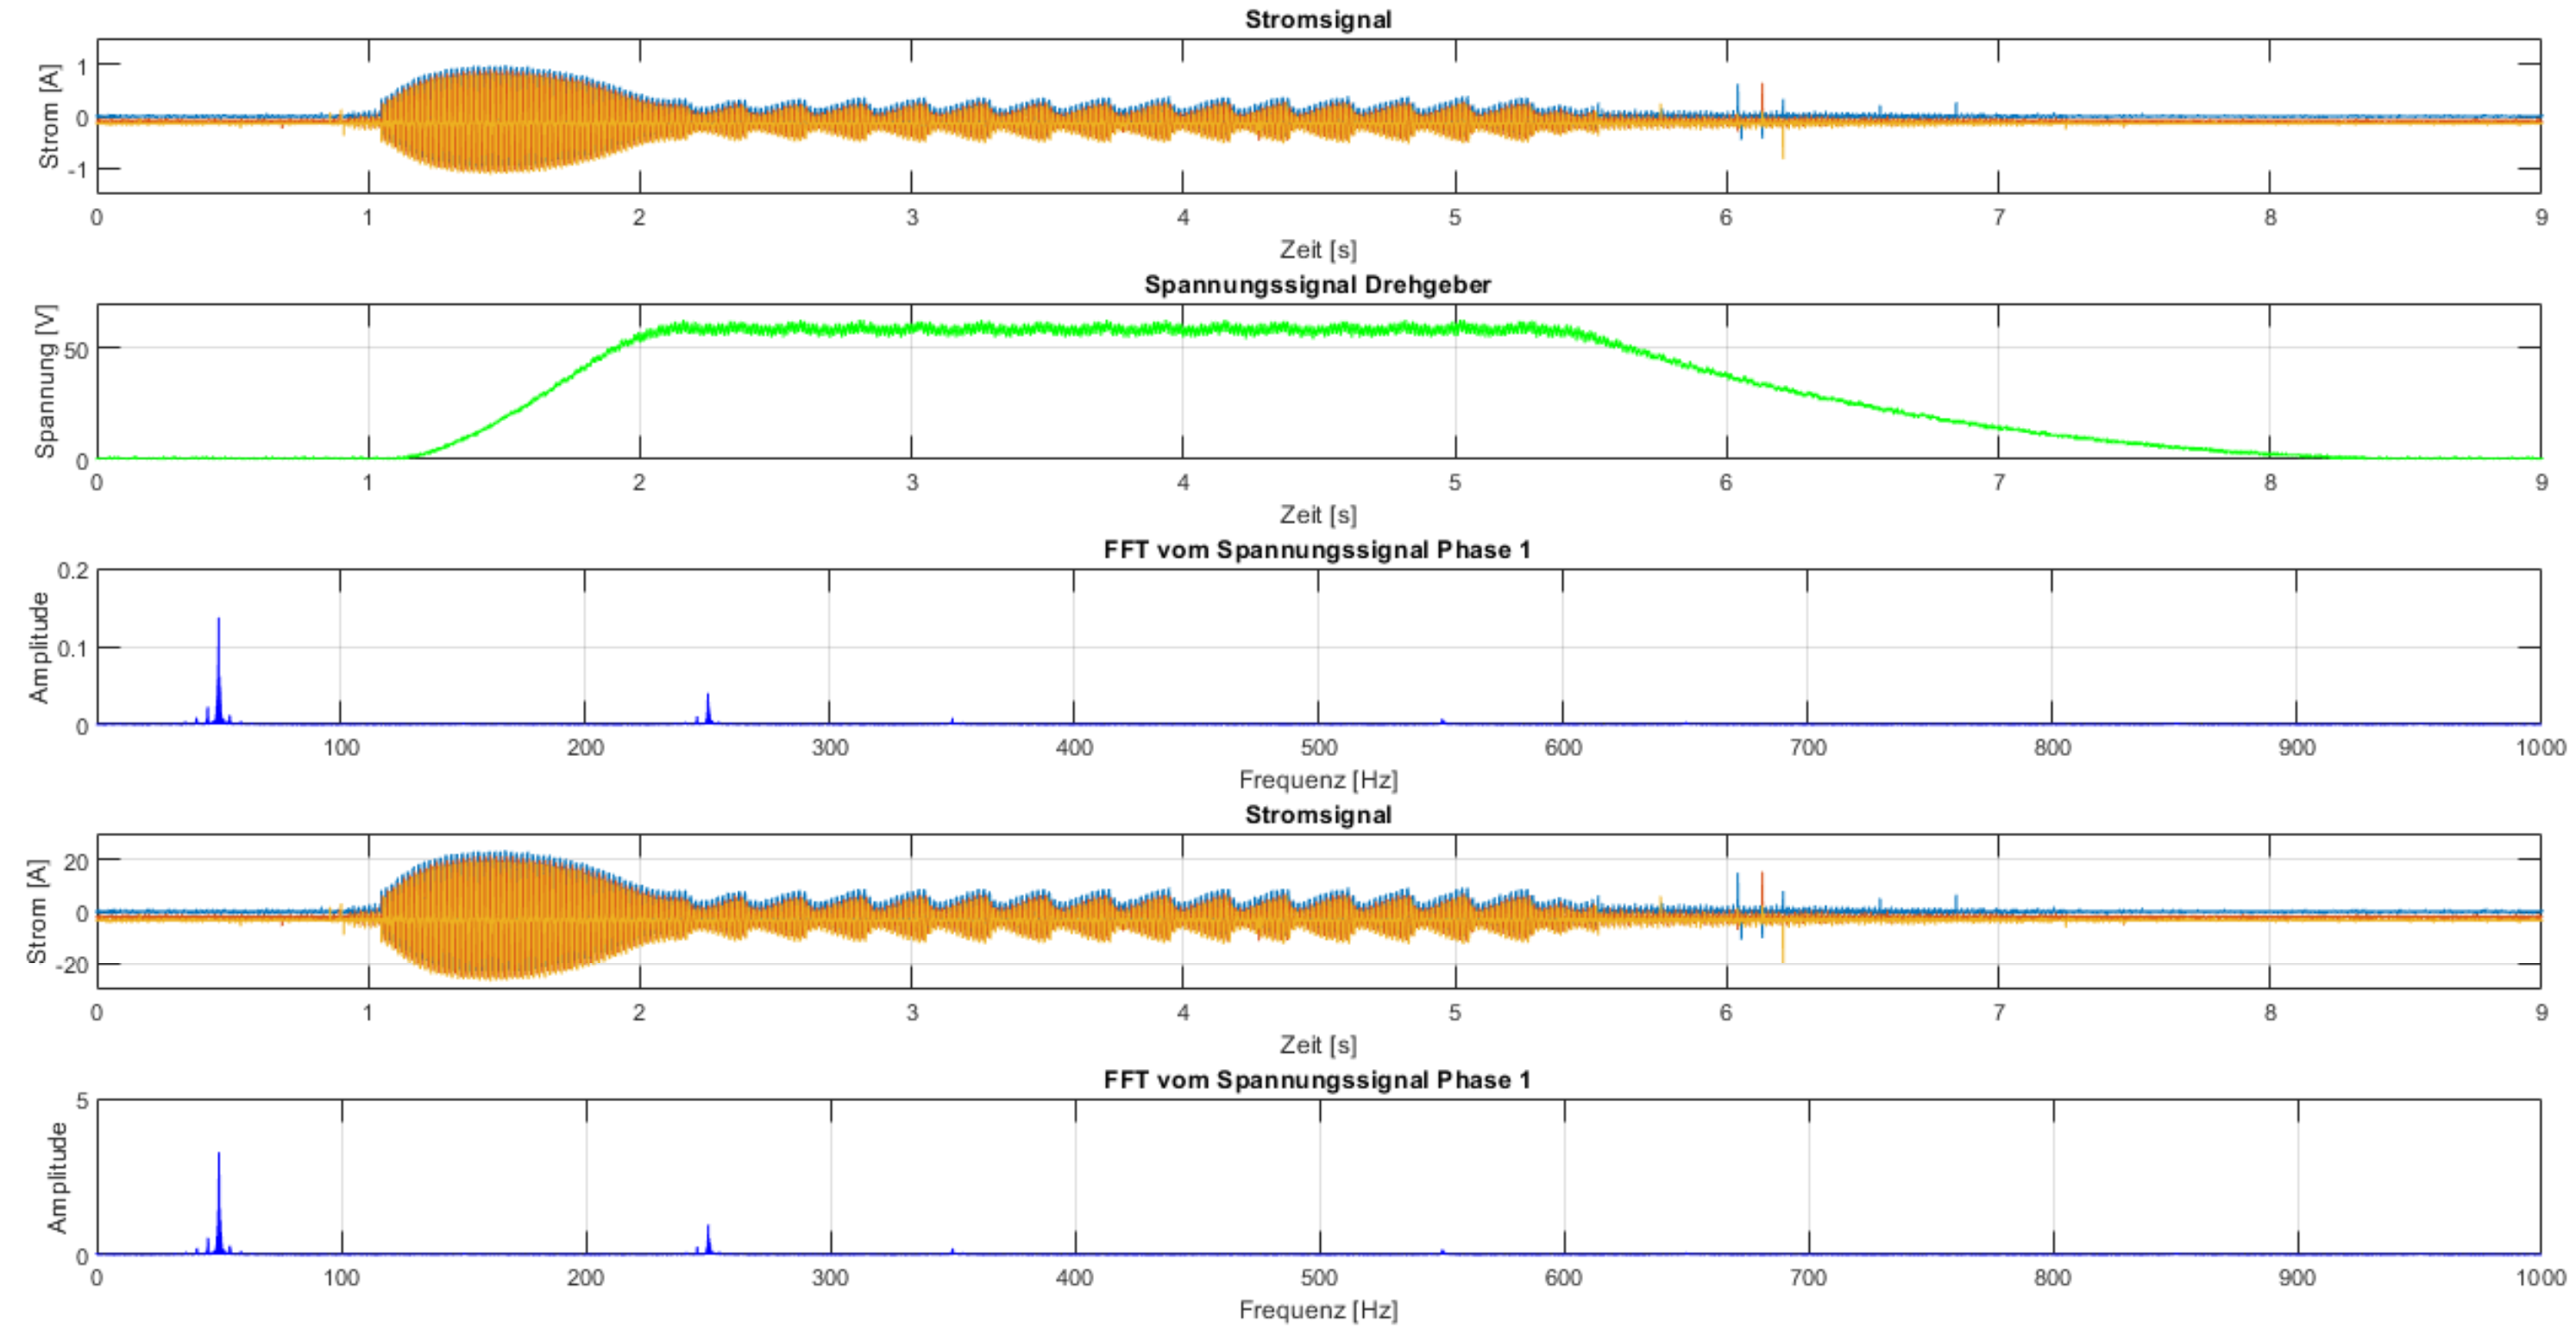
\includegraphics[width=\textwidth]{Messung_ASM_Phas_90grad_stroeme}	
	\caption{Messung mit Phasenanschnitt 90\textdegree}\label{fig:Mess_Phas_90grad_stroeme}
\end{figure}

\newpage
\subsubsection*{Sanft-Anlasser langsam}
\begin{figure}[ht!]
	\centering
	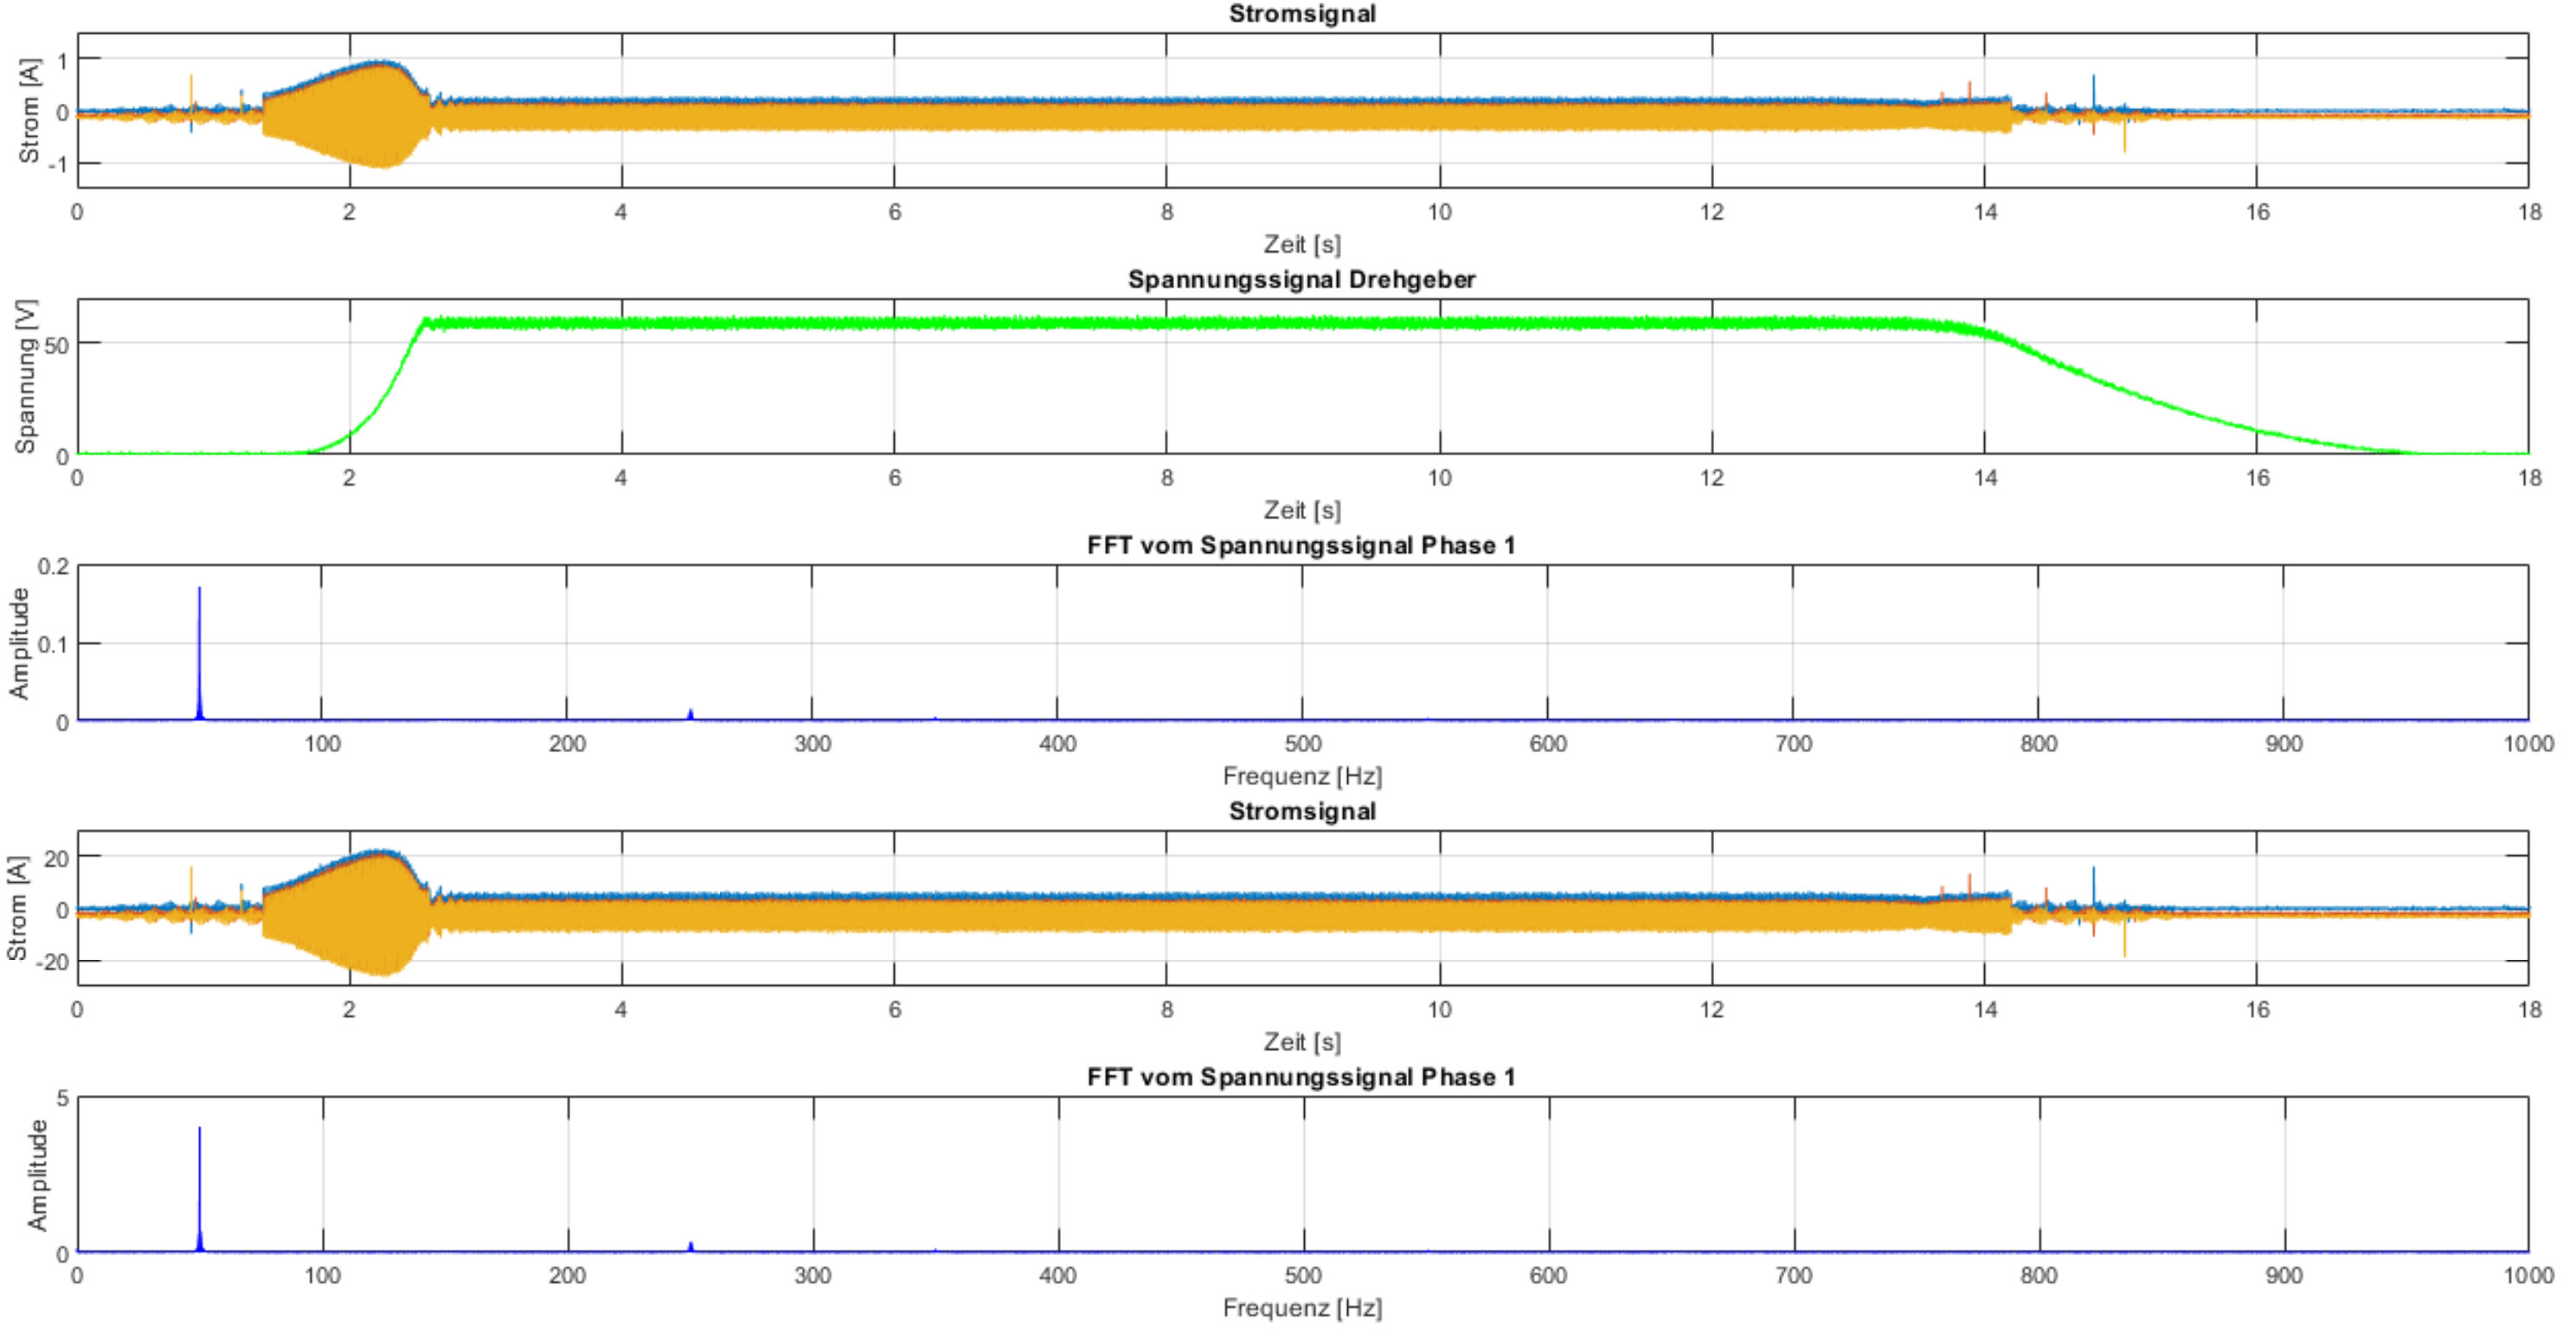
\includegraphics[width=\textwidth]{Messung_ASM_Sanft_langsam_stroeme}	
	\caption{Messung mit Sanft-Anlasser langsam}\label{fig:Mess_Sanft_langsam_stroeme}
\end{figure}




%\subsubsection{Schwingungspaketsteuerung mit Last in Stern}
%Für die Messung mit der Schwingungspaketsteuerung wurde eine Einschaltzeit von 0.5 Sekunden und eine Ausschaltzeit von 0.2 Sekunden gewählt. Die Ausschaltzeit darf nicht kürzer sein, da die Spannungsverstärkerschaltung und den Thyristorsteller eine Zeitverzögerung darstellen und so die Spannung nicht sofort ein- oder ausgeschaltet wird. Wenn die Ausschaltzeit kürzer ist, geht die Spannung zwischen den Paketen nicht auf \SI{0}{V}. 
%\begin{figure}[ht!]
%	\centering
%	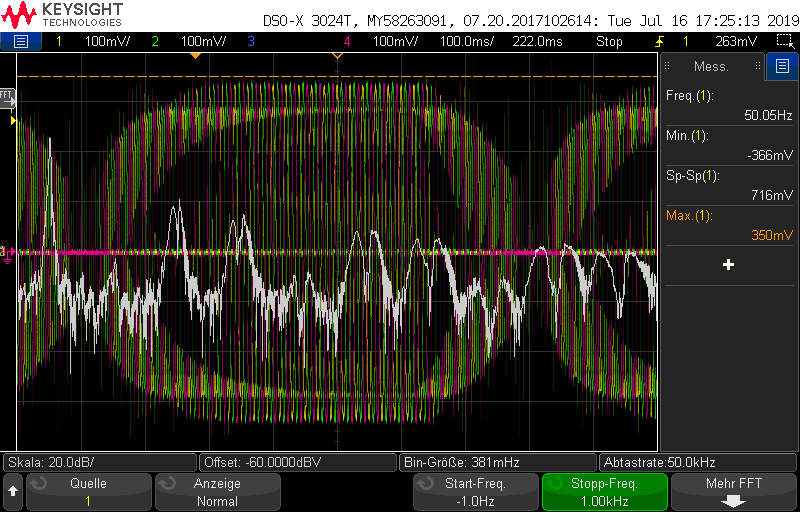
\includegraphics[width=0.7\textwidth]{Schwingungspaket_kurz.png}	
%	\caption{Das Spannungssignal aller Phasen bei Schwingungspaketsteuerung mit FFT}\label{fig:Mess_Schwing_kurz}
%\end{figure}
%
%Das FFT zeigt entgegen den Erwartungen aus der Theorie fast keine Subharmonische auf. Dafür sind Harmonische und Zwischehamrnische sehr ausgeprägt. Sehr gut zu sehen ist die Grundfrequenz von \SI{50}{Hz}, der erste Peak von der linken Seite. Dies ist darauf zurückzuführen, dass nicht direkt ein- und ausgeschaltet wird und so einem Sanft-Anlass ähnelt. Dies dominiert gegenüber dem harten Ein- und Ausschalten, welches die Subharmonische hervorrufen würde.
%\newpage
%\subsection{Phasenanschnittsteuerung mit 2 Thyristoren mit Last in Stern}
%Für die Sparansteuerung wurde ein Winkel von 90\textdegree \hspace{0.02cm} gewählt. 
%
%\begin{figure}[ht!]
%	\centering
%	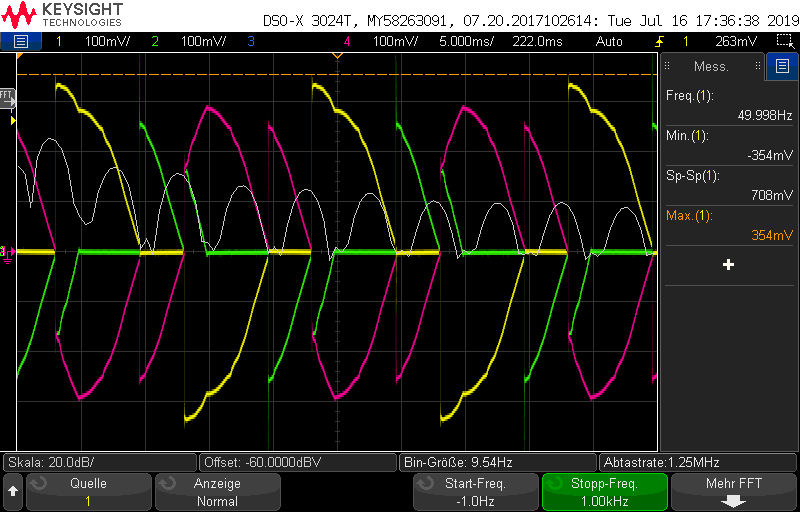
\includegraphics[width=0.7\textwidth]{2phas_90grad_kurz.png}	
%	\caption{Das Spannungssignal aller Phasen bei Schwingungspaketsteuerung mit FFT}\label{fig:Mess_2phas_kurz}
%\end{figure}
%
%
%\subsection{Phasenanschnittsteuerung mit 1 Thyristor mit Last in Stern}
%Für die Sparansteuerung wurde ein Winkel von 90\textdegree gewählt. 
%
%\begin{figure}[ht!]
%	\centering
%	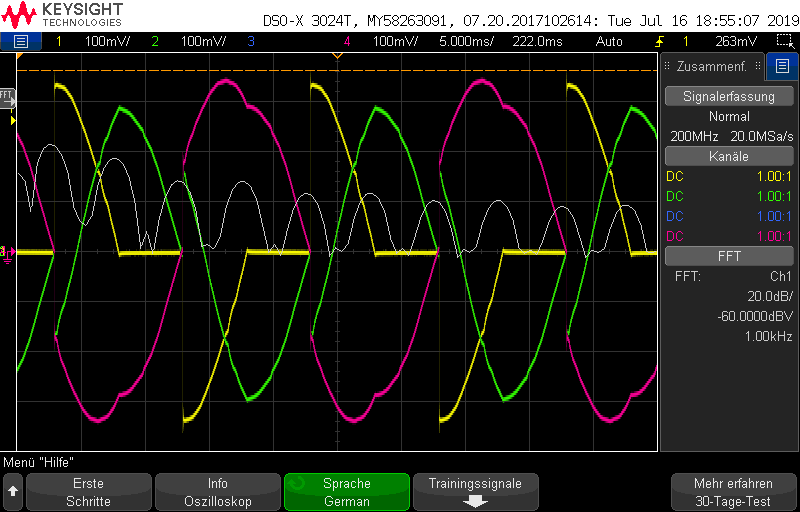
\includegraphics[width=0.7\textwidth]{1phas_90grad_kurz.png}	
%	\caption{Das Spannungssignal aller Phasen bei Schwingungspaketsteuerung mit FFT}\label{fig:Mess_1phas_kurz}
%\end{figure}




